\documentclass[12pt,a4paper,final]{report}
\usepackage[utf8]{inputenc}
\usepackage[T2A]{fontenc}
\usepackage[russian]{babel}
\usepackage{graphicx}
\usepackage{amsmath}
\usepackage{amssymb}
\usepackage{bm}
\usepackage[left=3cm,right=3cm,top=2cm,bottom=2cm]{geometry}

\usepackage{mathtools}
\newcommand\iid{\stackrel{\mathclap{\normalfont\mbox{iid}}}{\sim}}
\newcommand{\hbv}{\hat{\mathbf{v}}}
\newcommand{\seh}{\widehat{\text{se}}}
\newcommand{\sew}{\widetilde{\text{se}}}
\newcommand{\X}{\mathbf X}
\newcommand{\tx}[1]{\text{#1}}
\newcommand{\rse}{\text{RSE}}
\newcommand{\betah}{\hat \beta}
\newcommand{\rloess}{\hat{r}_\tx{loess}}
\newcommand{\rquad}{\hat{r}_\tx{quad}}
\newcommand{\thetahat}{\hat \theta}
\newcommand{\bca}{\mathrm{BC}_a}
\newcommand{\abc}{\mathrm{ABC}}
\newcommand{\prob}[1]{\mathrm{Prob}\left\{#1\right\}}
\newcommand{\xest}[1]{x_1^*,x_2^*,\ldots,x_{#1}^*}
\newcommand{\xes}[1]{x_1,x_2,\ldots,x_{#1}}
\newcommand{\ies}[1]{1,2,\ldots,#1}
\newcommand{\equd}{\dot{=}}
\newcommand{\summ}[2]{\sum_{#1}^{#2}}
\newcommand{\mbf}{\mathbf}
\newcommand{\what}[1]{\widehat{#1}}


\setcounter{chapter}{1}


\title{Введение в Бутстреп}
% \author{st013309}
\date{2021}

\begin{document}

\maketitle

\tableofcontents

\chapter{Точность выборочного среднего }
Бутстреп - это компьютерный метод определения точности статистических оценок. Основная идея, лежащая в основе бутстрепа, очень проста и насчитывает как минимум два столетия. После ознакомления с некоторыми справочными материалами в этом отчете описывается метод бутстрепа и его применение для решения некоторых реальных задач анализа данных. В этой главе, помимо предварительного ознакомления с бутстрепом, рассматриваются некоторые фундаментальные идеи статистики. Основное внимание уделяется одному примеру статистики, для оценки точности котрой не нужен компьютер: выборочное среднее. Начнем с простого примера, касающегося средних и их расчетной точности. 

В таблице 2.1 показаны результаты небольшого эксперимента, в котором 7 из 16 мышей были случайным образом выбраны для получения нового лечения, а остальные 9 были отнесены к группе без лечения (контрольной). Лечение было направлено на продление выживаемости после тестовой операции. В таблице показано время выживания после операции в днях для всех 16 мышей. \newline

\noindent
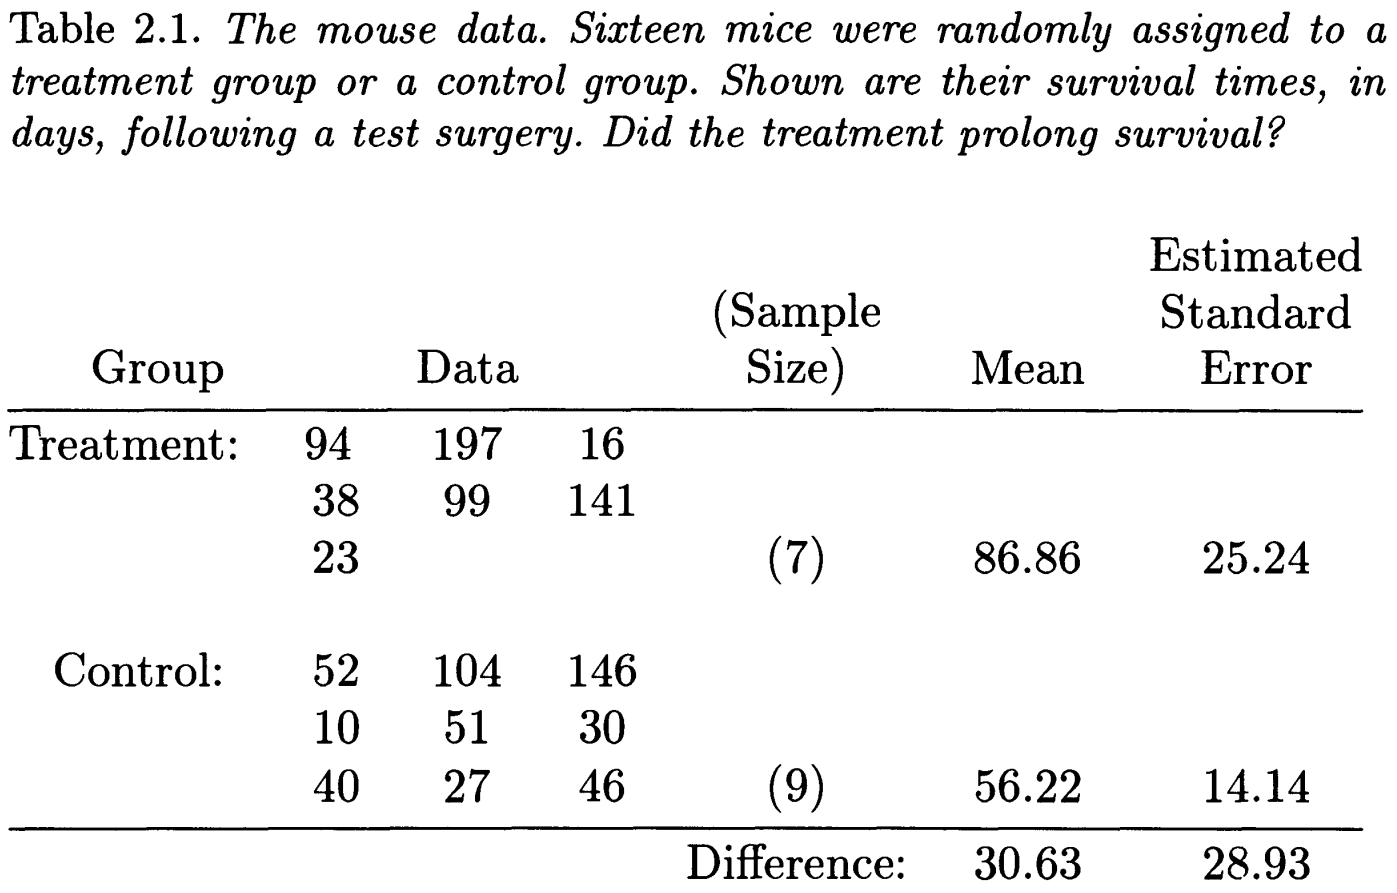
\includegraphics[width=\linewidth]{1/t1.png}
\newline

Продлило ли лечение выживаемость? Сравнение средних значений для двух групп дает предварительные основания для положительного ответа. Обозначим через $x_1,x_2,\ldots x_7$ продолжительность жизни в группе с лечением, соотв. $x_1=94,x_2=197,\ldots,x_7=23$, а через $y_1,y_2,\ldots y_9$ продолжительность жизни в контрольной группе. Групповые выборочные средние равны
\begin{equation}
    \overline x = \sum_{i=1}^7 x_i/7 = 86.86 \quad \texttt{и} \quad \overline y = \sum_{i=1}^9 y_i/9 = 56.22,
\end{equation}
таким образом разность $\overline x - \overline y$ равна $30.63$, что предполагает значительный эффект продления жизни при лечении.

Но насколько точны эти оценки? В конце концов, средние (2.1) основаны на небольших выборках, всего 7 и 9 мышей соответственно. Чтобы ответить на этот вопрос, нам нужна оценка точности выборочных средних $\overline x$ и $\overline y$). Для выборочных средних и по существу только для выборочных средних формулу точности получить легко. 

Расчетная стандартная ошибка среднего $\overline x$ на основе $n$ независимых наблюдений $x_1, x_2,\ldots, x_n$, $\overline x =\sum_{i=1}^n x_i/n$, определяется формулой 
\begin{equation}
    \sqrt{\frac{s^2}{n}},
\end{equation}
где $s^2=\sum_{i=1}^n (x_i-\overline x)^2/(n-1)$. (Эта формула и стандартные ошибки в целом обсуждаются более подробно в главе 4.) Стандартная ошибка любой оценки определяется как квадратный корень из ее дисперсии, то есть среднеквадратичная изменчивость оценки вокруг ее математического ожидания. Это наиболее распространенная мера точности оценок. Грубо говоря, оценка отличается от своего истинного значения менее чем на одну стандартную ошибку примерно в 68\% случаев и менее чем на две стандартные ошибки примерно в 95\% случаев.

Если бы оценочные стандартные ошибки в эксперименте на мышах были очень малы, скажем, менее 1, тогда мы бы знали, что $\overline x$ и $\overline y$ были близки к их истинным значениям и что наблюдаемая разница в 30,63, вероятно, была хорошей оценкой истинного увеличения выживаемости при лечении. С другой стороны, если формула (2.2) дает большие оценочные стандартные ошибки, скажем 50, тогда оценка разности будет слишком неточной, чтобы на нее можно было полагаться. 

Фактическая ситуация показана справа в Таблице 2.1. Расчетные стандартные ошибки, рассчитанные по (2.2), составляют 25,24 для $\overline x$ и 14,14 для $\overline y$. Стандартная ошибка для разности $\overline x - \overline y$ равна $28,93 = \sqrt{25,24^2 + 14,14^2}$ (поскольку дисперсия разности двух независимых величин является суммой их дисперсий). Мы видим, что наблюдаемая разница 30,63 составляет всего $30,63 / 28,93 = 1,05$ стандартной ошибки разности. Читатели, знакомые с теорией проверки гипотез, сочтут это незначимым результатом, который может легко возникнуть случайно, даже если лечение действительно не имело никакого эффекта. 

Обычно стандартные ошибки являются отличным первым шагом к критическому осмыслению статистических оценок. К сожалению, стандартные ошибки имеют серьезный недостаток: для большинства статистических оценок, отличных от среднего, не существует формулы, подобной (2.2), для получения стандартных ошибок. Другими словами, трудно оценить точность оценки, отличной от оценки среднего.

Предположим, например, что мы хотим сравнить две группы в таблице 2.1 по их медианам, а не по их средним значениям. Медианы составляют 94 для лечения и 46 для контроля, что дает разницу в 48, что значительно больше, чем разница средних значений. Но насколько точны эти медианы? Ответы на такие вопросы - вот где вступают в игру бутстреп и другие компьютерные методы. В оставшейся части этой главы дается краткий обзор начальной оценки стандартной ошибки - метода, который будет полностью обсуждаться в следующих главах. 

Предположим, что мы наблюдаем независимые данные $x_1, x_2,\ldots, x_n$, для удобства обозначенные вектором $X = (x_1, x_2, \ldots, x_n)$, по которым мы вычисляем интересующую статистику $s(X)$. Например, данные могут быть наблюдениями контрольной группы $n = 9$ в таблице 2.1, а $s(X)$ может быть средним по выборке. 

Бутстреп оценка стандартной ошибки, изобретенная Эфроном в 1979 году, выглядит совершенно иначе, чем (2.2), но на самом деле они тесно связаны. Бутстреп выборка $X^* = (x^*_i, x^*_2,\ldots, x^*_n)$ получается путем случайного выбора с возвращением $n$ точек из исходных данных $x_1, x_2,\ldots, x_n$. Например, при $n = 7$ мы можем получить $X^* = (x_5, x_7, x_5, x_4, x_7, x_3, x_1)$· 
\newline

\noindent
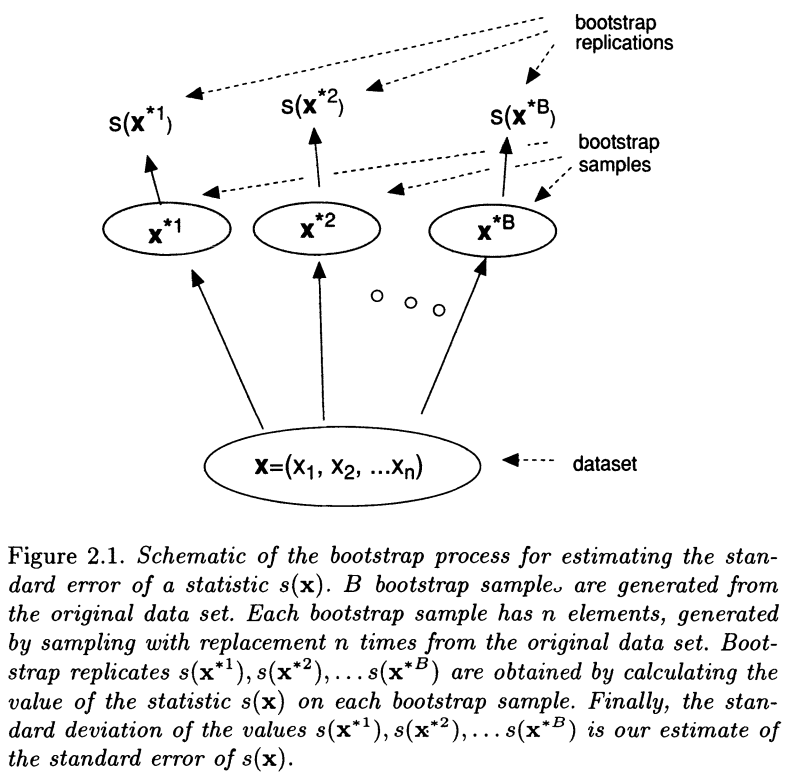
\includegraphics[width=\linewidth]{1/f1.png}
\newline

Рисунок 2.1 представляет собой схему процесса бутстрепа. Алгоритм бутстрепа начинается с генерации большого количества независимых бутстреп выборок $X^{*1}, X^{* 2},\ldots, X^{*B}$, каждая размером n. Типичные значения для B, количества бутстреп выборок, находятся в диапазоне от 50 до 200 для оценки стандартной ошибки. Каждой бутстреп выборке соответствует бутстреп репликация $s (X^{* b})$, посчитанная для $X^{* b}$. Если $s(X)$ - это, например, медиана выборки, то $s (X^*)$ - это медиана бутстреп выборки. Бутстреп оценка стандартной ошибки - это стандартное отклонение бутстреп репликаций  
\begin{equation}
    \hat{se}_{boot}=\left\{\sum_{b=1}^B [s(X^{*b})-s(\cdot)]^2/(B-1)\right\}^{\frac{1}{2}},
\end{equation}
где $s(\cdot)=\sum_{b=1}^B s(X^{*b})/B$. Предположим, что $s(X)=\overline X$. В этом случае стандартная теория вероятностей говорит нам, что, когда B становится очень большим, формула (2.3) приближается к  
\begin{equation}
    \left\{\sum_{i=1}^n (x_i-\overline x)^2/n^2\right\}^{\frac{1}{2}}.
\end{equation}

Это почти то же самое, что и формула (2.2). Мы могли бы сделать это точно таким же, умножив определение (2.3) на множитель $[n / (n-1)] ^\frac{1}{2}$, но в этом нет практического смысла. 
\newline

\noindent
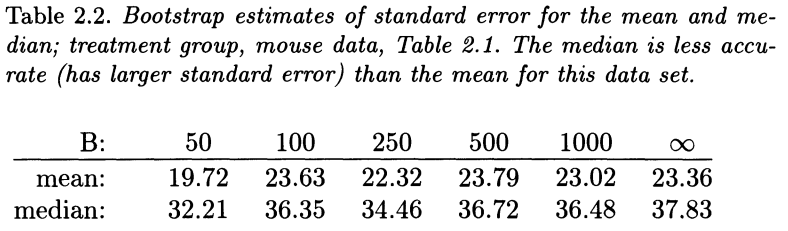
\includegraphics[width=\linewidth]{1/t2.png}
\newline

В таблице 2.2 показаны бутстрап оценки стандартной ошибки для среднего и медианы для данных экспериментальной группы мышей из таблицы 2.1. Стандартные ошибки уменьшаются до предельных значений по мере увеличения числа бутстраповых выборок $B$. Предельное значение $23,36$ для среднего получается из (2.4). Формула для предельного значения $37,83$ для стандартной ошибки медианы довольно сложна. 

Теперь мы можем оценить точность разницы медиан между двумя группами. Описанная выше бутстреп процедура, примененная к контрольной группе, дала оценку стандартной ошибки $11,54$ на основе $B = 100$ повторений ($B = \infty$ дало $9,73$). Следовательно, используя $B = 100$, наблюдаемая разница в $48$ имеет расчетную стандартную ошибку $\sqrt{36,35^2 + 11,54^2} = 38,14$, и, следовательно, $48 / 38,14 = 1,26$ стандартной ошибки. Это больше, чем наблюдаемая разница в средних, но все же незначимо. 

Для большинства статистических данных у нас нет формулы для предельного значения стандартной ошибки, но на самом деле формула не нужна. Вместо этого мы используем числовой вывод бутстреп программы для некоторого удобного значения B. Легко написать бутстреп программу, которая работает для любой вычислимой статистики $s (X)$. Имея эти программы, аналитик данных может свободно использовать любую статистику, независимо от ее сложности, с уверенностью, что он или она также будет иметь разумное представление о точности оценки. Применение бутстрепа стало доступным, поскольку компьютеры стали мощнее и дешевле. 
Стандартные ошибки - это простейшие меры статистической точности. В последующих главах показано, как бутстреп методы могут оценивать более сложные меры точности, такие как смещения, ошибки прогнозирования и доверительные интервалы. Бутстрепированные доверительные интервалы увеличивают вычислительную нагрузку еще в 10 раз. Результатом всех этих вычислений является увеличение количества статистических проблем, которые могут быть проанализированы, сокращение допущений анализа и устранение рутинных, но утомительных теоретических расчетов, обычно связанных с оценкой точности. 

\chapter{Случайные выборки и вероятности}
\section{Введение}

Статистика - это теория накопления информации, особенно информации, поступающей постепенно. Типичная статистическая ситуация была проиллюстрирована данными по мышам в Таблице 2.1. Ни одна мышь не предоставляет много информации, поскольку индивидуальные результаты очень различаются, но семь или девять мышей, взятых вместе, начинают быть весьма информативными. Статистическая теория касается лучших способов извлечения этой информации. Теория вероятностей обеспечивает математическую основу для статистических выводов. В этой главе рассматривается простейшая вероятностная модель, используемая для моделирования случайных данных: случай, когда наблюдения представляют собой случайную выборку из одной неизвестной совокупности, свойства которой мы пытаемся узнать из наблюдаемых данных. 
\section{Случайные выборки}

Проще всего визуализировать случайные выборки в терминах конечной совокупности или «вселенной» $\mathbf{U}$ отдельных единиц $U_1, U_2, \ldots, U_n$, любая из которых с равной вероятностью будет выбрана в одном случайном розыгрыше. В состав единиц могут входить все зарегистрированные избиратели в районе, подвергающемся политическому обследованию, все мужчины, которые предположительно могут быть выбраны для медицинского эксперимента, все средние школы в Соединенных Штатах и т.д. У отдельных единиц есть свойства, которые нам нужны. чтобы узнать, например, о политических взглядах, времени выживания в медицине или количестве выпускников. Слишком сложно и дорого исследовать каждую единицу в $\mathbf{U}$, поэтому мы выбираем для наблюдения случайную выборку управляемого размера. 

Случайная выборка размера $n$ определяется как набор из $n$ единиц $u_1, u_2,\ldots, u_n$, выбранных случайным образом из $\mathbf{U}$. В принципе, процесс выборки происходит следующим образом: устройство случайных чисел независимо выбирает целые числа $j_1 , j_2,\ldots, j_n$, каждое из которых равно любому значению от 1 до $N$ с вероятностью $1 / N$. Эти целые числа определяют, какие члены $\mathbf{U}$ выбраны для случайной выборки, $u_1 = U_{j_1}, u_2 = U_{j_2},\ldots,u_n=U_{j_n}$. На практике процесс отбора редко бывает таким аккуратным, и совокупность $\mathbf{U}$ может быть плохо определена, но концептуальная структура случайной выборки по-прежнему полезна для понимания статистических выводов. (Методология хорошего экспериментального дизайна, например, случайное распределение выбранных единиц в экспериментальную или контрольную группы, как это было сделано в эксперименте на мышах, помогает сделать теорию случайной выборки более применимой к реальным ситуациям, подобным той, что представлена в таблице 2.1.) 

Наше определение случайной выборки позволяет одной единице $U_i$ появляться в выборке более одного раза. Мы могли бы избежать этого, настаивая на том, чтобы целые числа $j_1, j_2,\ldots, j_n$ были различными, что называется <<выборкой без замены>>. Чуть проще разрешить повторы, то есть <<выборку с заменой>>, как в предыдущем абзаце. Если размер случайной выборки $n$ намного меньше, чем размер генеральной совокупности $N$, как это обычно бывает, вероятность повторения выборки в любом случае будет мала. См. Проблему 3.1. Случайная выборка всегда означает выборку с заменой в дальнейшем, если не указано иное. 

Выбрав случайную выборку $u_1, u_2,\ldots, u_n$, мы получаем одно или несколько представляющих интерес измерений для каждой единицы. Пусть $x_i$ обозначает измерения для единицы $u_i$. Наблюдаемые данные представляют собой набор измерений $x_1, x_2,\ldots, x_n$. Иногда мы будем обозначать наблюдаемые данные $(x_1, x_2, \ldots, x_n)$ одним символом $X$. 

Мы можем представить себе, как проводить измерения для каждого члена $U_1, U_2, \ldots ,U_N$ из $\mathbf{U}$, получая значения $X_1, X_2, \ldots, X_N$. Это можно было бы назвать переписью $U$. 

Символ $\mathbf{X}$ будет обозначать перепись измерений $(X_1, X_2,\ldots, X_N)$. Мы также будем называть $\mathbf{X}$ совокупностью измерений или просто совокупностью и называть $X$ случайной выборкой размера $n$ из $\mathbf{X}$. На самом деле мы обычно не можем позволить себе провести перепись, поэтому мы взяли случайную выборку. Цель статистического вывода -- сказать, что мы узнали о популяции $\mathbf{X}$ из наблюдаемых данных $X$. В частности, мы будем использовать бутстреп, чтобы сказать, насколько точно статистика, вычисленная из $x_1, x_2,\ldots, x_n$ (например, медиана выборки), оценивает соответствующее количество для всей генеральной совокупности. 
\newline

\noindent
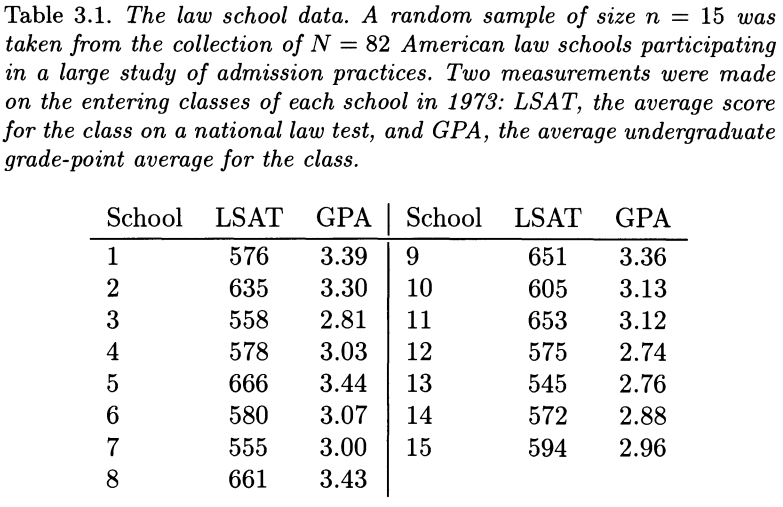
\includegraphics[width=\linewidth]{2/t21.png}
\newline

В таблице 3.1 показана случайная выборка размером $n = 15$, составленная из 82 американских юридических школ. Фактически показаны два измерения, проведенные для поступающих в 1973г. для каждого учебного заведения в выборке: LSAT, средний балл класса на экзамене по национальному праву, и GPA, средний балл бакалавриата, полученный студентами. В этом случае измерение $x_i$ на $u_i$, $i$-м члене выборки, представляет собой пару 
\begin{equation*}
    x_i=(LSAT_i, GPA_i)\quad i=1,2,\cdots,15
\end{equation*}
Наблюдаемые данные $x_1, x_2,\ldots, x_n$ представляют собой набор из 15 пар чисел, показанных в таблице 3.1. 

Этот пример является искусственным, потому что перепись данных $X_1, X_2,\cdots, X_82$ действительно была проведена. Другими словами, LSAT и GPA доступны для всей совокупности $N = 82$ школ. На Рисунке 3.1 показаны данные переписи и выборочные данные. В таблице 3.2 приведены все измерения $N$. 
\newline

\noindent
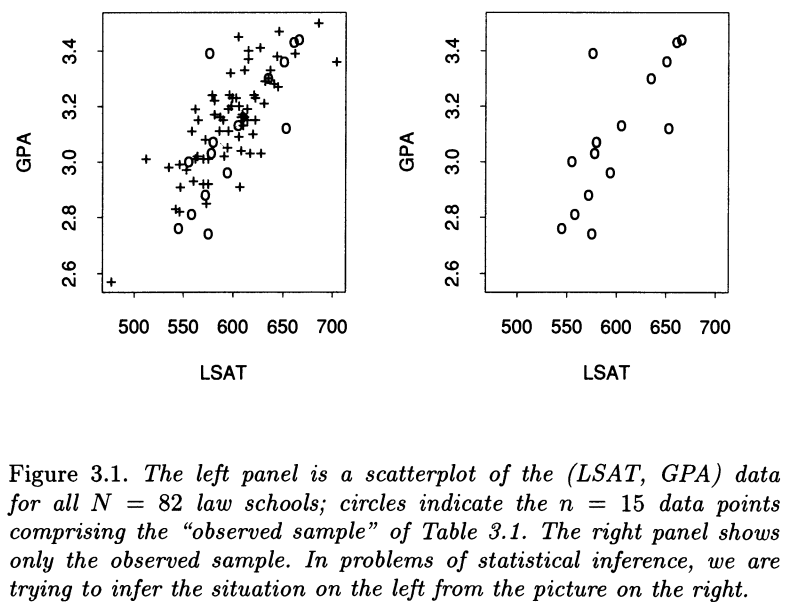
\includegraphics[width=\linewidth]{2/f31.png}
\newline

В реальной статистической задаче, такой как в таблице 3.1, мы увидим только выборочные данные, из которых мы попытаемся сделать вывод о свойствах совокупности. Например, рассмотрим 15 баллов LSAT в наблюдаемой выборке. Они имеют среднее значение $600.27$ с расчетной стандартной ошибкой $10.79$, основанной на данных в таблице 3.1 и формуле (2.2). Вероятность того, что истинное среднее значение LSAT, среднее для всей генеральной совокупности, из которой были взяты наблюдаемые данные, составляет около 68\%, находится в интервале $600.27 \pm 10.79$. 

Мы можем проверить этот результат, поскольку имеем дело с искусственным примером, для которого известны полные данные о населении. Среднее значение всех 82 значений LSAT составляет $597.55$, оно лежит в пределах прогнозируемого доверительного интервала $600.27 \pm 10.79$. 
\newline

\noindent
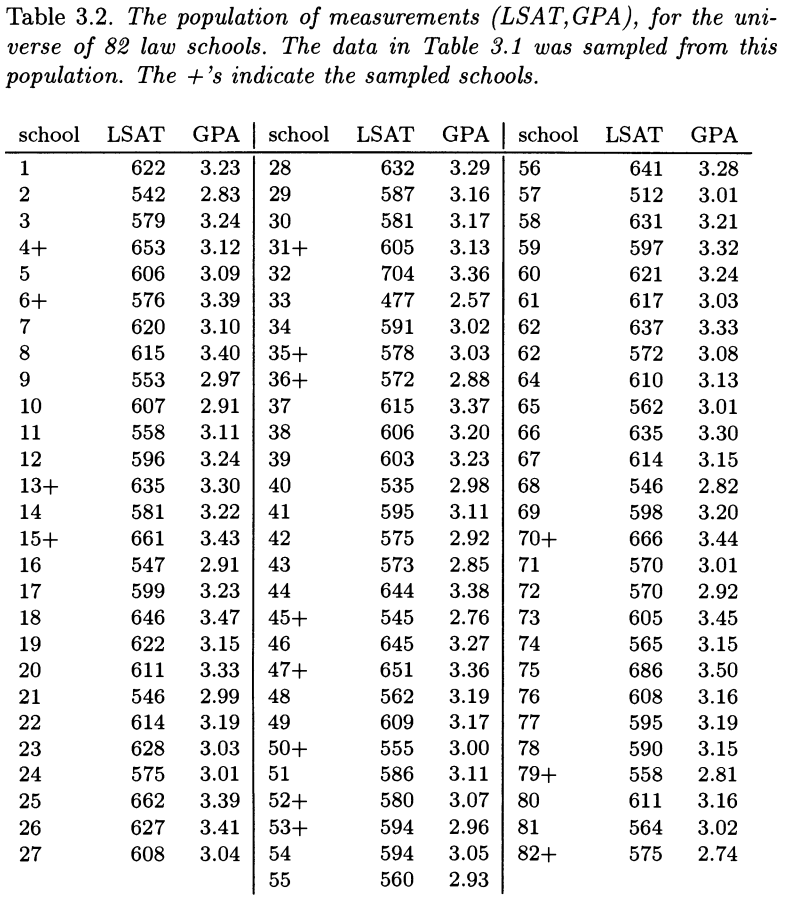
\includegraphics[width=\linewidth]{2/t32.png}
\newline
\section{Теория вероятностей}

Статистический вывод касается обучения на опыте: мы наблюдаем случайную выборку $\mathbf{x} = (x_1, x_2, \cdots, x_n)$ и хотим вывести свойства полной совокупности $\mathbf{X} = (X_1, X_2,\cdots, X_N)$, которая дала образец. Теория вероятностей идет в противоположном направлении: из состава популяции $\mathbf{X}$ мы выводим свойства случайной выборки $\mathbf{x}$ и статистики, вычисляемой по $\mathbf{x}$. Статистический вывод как математическая наука был разработан почти исключительно в терминах теории вероятностей. Здесь мы кратко рассмотрим некоторые фундаментальные концепции вероятности, включая распределения вероятностей, ожидания и независимость. 

В качестве первого примера пусть $x$ представляет результат броска правильной кости, поэтому $x$ с равной вероятностью будет 1, 2, 3, 4, 5 или 6. Мы запишем это в вероятностной нотации как 
\begin{equation}
    Prob\{x=k\}=1/6\qquad for\quad k=1,2,3,4,5,6.
\end{equation}

Случайное число, такое как $x$, часто называется случайной величиной. 

Вероятности - это идеализированные или теоретические пропорции. Мы можем представить себе пространство $\mathbf(U) = \{U_1 U_2, \cdots, U_N\}$ возможных бросков кубика, где $U_j$ полностью описывает физический акт j-го броска с соответствующими результатами $\mathbf{X} = (X_1, X_2,\cdots, X_N)$. Здесь $N$ может быть очень большим или даже бесконечным. Выражение $Prob\{x = 5\} = 1/6$ означает, что случайным образом выбранный член $\mathbf{X}$ имеет 1/6 шанс быть равным 5, или, проще говоря, 1/6 членов $\mathbf{X}$ равняется 5. Обратите внимание что такие вероятности, как пропорции, никогда не могут быть меньше 0 или больше 1. 

Для удобства обозначений определим частоты $f_k$, 
\begin{equation}
    f_k=Prob\{x=k\},
\end{equation}
так что у справедливой кости $f_k = 1/6$ для $k = 1, 2, \cdots, 6$. Распределение вероятностей случайной величины $x$, которую мы обозначим $F$, является любым полным описанием вероятностного поведения $x$. $F$ также называется распределением вероятностей популяции $\mathbf{X}$. Здесь мы можем взять $F$ как вектор частот 
\begin{equation}
    F=(f_1,f_2,\cdots,f_6)=(1/6, 1/6, \cdots,1/6).
\end{equation}
Несправедливым будет кубик, для которого $F$ не равно $(1/6, 1/6, \cdots,1/6)$. 

Некоторые распределения вероятностей возникают настолько часто, что получили специальные названия. Говорят, что случайная величина $x$ имеет биномиальное распределение с размером $n$ и вероятностью успеха $p$, что обозначается 
\begin{equation}
    x\sim Bi(n,p),
\end{equation}
если его частоты 
\begin{equation}
    f_k=C_n^kp^k(1-p)^{n-k}\quad for\quad k=0,1,2,\cdots,n.
\end{equation}
Здесь $n$ -- положительное целое число, $p$ -- число от 0 до 1, а $C_n^k$ -- биномиальный коэффициент $n! / [K! (n-k)!]$. На рисунке 3.2 показано распределение $F = (f_0, f_1, \cdots, f_n)$ для $x \sim Bi (n, p)$, при $n = 25$ и $p = 0.25, 0.50$ и $0.90$. Мы также пишем $F = Bi (n, p)$ для обозначения ситуации (3.4). 
\newline

\noindent
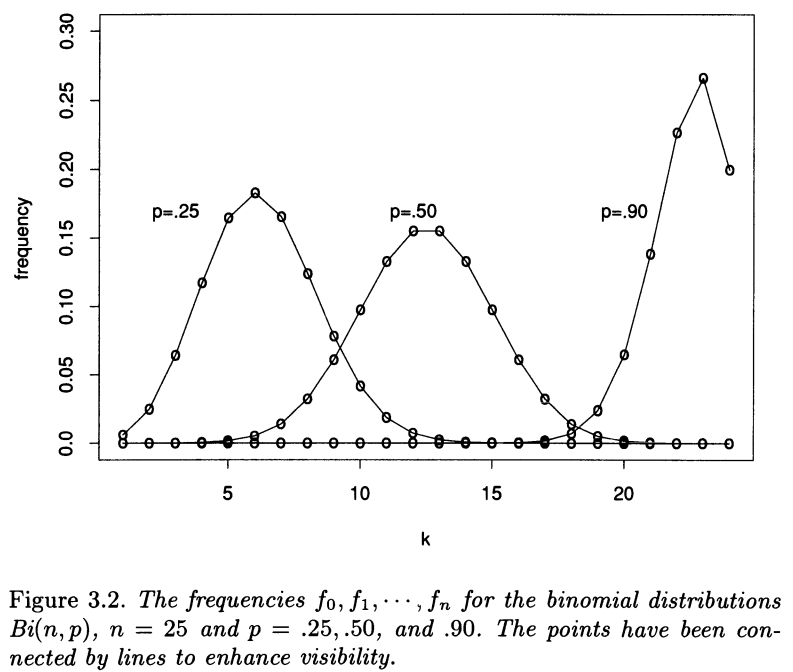
\includegraphics[width=\linewidth]{2/f32.png}
\newline

Пусть $A$ -- набор целых чисел. Тогда вероятность того, что $x$ принимает значение в $A$, или, проще говоря, вероятность $A$, равна 
\begin{equation}
    Prob\{x\in A\}=Prob\{A\}=\sum_{k\in A}f_k.
\end{equation}
Например, если $A = \{1, 3, 5, \cdots, 25\}$ и $x \sim Bi (25, p)$, то $Prob \{A\}$ -- это вероятность того, что биномиальная случайная величина размера 25 и вероятность успеха $p$ равно нечетному целому числу. Заметьте, что, поскольку $f_k$ -- это теоретическая доля раз, когда $x$ равно $k$, сумма $\sum_{k\in A}f_k = Prob \{A\}$ -- это теоретическая доля раз, когда $x$ принимает свое значение в $A$. 

Выборочное пространство $x$, обозначенное $S_x$, представляет собой набор возможных значений $x$. Для правильного кубика $S_x = \{1, 2, \cdots, 6\}$, а $S_x = \{0, 1, 2, \cdots, n\}$ для распределения $Bi (n, p)$. По определению $x$ встречается в $S_x$ каждый раз, то есть с теоретической пропорцией 1, поэтому
\begin{equation}
    Prob\{S_x\}=\sum_{k\in S_x}f_k=1.
\end{equation}
Для любого распределения вероятностей целых чисел частоты $f_j$ являются неотрицательными числами, сумма которых равна 1. 

В наших примерах до сих пор пространство выборки $S_x$ было подмножеством целых чисел. Одна из удобных особенностей вероятностных распределений заключается в том, что их можно определять в довольно общих пространствах. Рассмотрим данные юридического факультета на Рисунке 3.1. Мы могли бы принять $S_x$ за положительный квадрант плоскости
\begin{equation}
    S_x=\mathbf{R}^{2+}=\{(y,z),y>0,z>0\}.
\end{equation}
(Сюда входят такие значения, как $x = (10^6, 10^9)$, но не повредит, если $S_x$ будет слишком большим.) Для подмножества $A$ из $S_x$ мы все равно будем писать $Prob \{A\}$, чтобы указать вероятность того, что $x$ встречается в $A$. 

Например, мы могли бы взять 
\begin{equation}
    A=\{(y,z):0<y<600,0<z<3.0\}.
\end{equation}
Юридическая школа $x \in A$, если ее входной класс 1973 года имел LSAT менее 600 и средний балл менее 3,0. В этом случае мы знаем полную популяцию $\mathbf{X}$; это 82 точки, указанные на левой панели рисунка 3.1 и в таблице 3.2. Из них 16 находятся в $A$, поэтому 
\begin{equation}
    Prob\{A\}=16/82=0.195.
\end{equation}
Здесь идеализированная пропорция $Prob \{A\}$ -- это действительная пропорция. Только в тех случаях, когда у нас есть полная генеральная совокупность, можно напрямую оценить вероятности как пропорции. 

Распределение вероятностей $F$ $x$ по-прежнему определяется как полное описание вероятностей $x$. В примере с юридической школой $F$ можно описать следующим образом: для любого подмножества $A$ из $S_x = \mathbf{R}^{2+}$, 
\begin{equation}
    Prob\{x\in A\}=\#\{X_j\in A\}/82,
\end{equation}
где $\# \{X_j \in A\}$ -- это 82 точки на левой панели рисунка 3.1, которые лежат в $A$. Другим способом сказать, что $F$ -- это дискретное распределение, полагая вероятность (или частоту) 1/82 на каждую из указанных 82 точек. 

Вероятности можно определять непрерывно, а не дискретно, как в (3.6) или (3.11). Самый известный пример -- нормальное (или гауссово, или колоколообразное) распределение. Определено, что случайная величина $x$ с действительными значениями имеет нормальное распределение со средним $\mu$ и дисперсией $\sigma^2$, записанное 
\begin{equation}
    x\sim N(\mu,\sigma^2)\quad or \quad F=N(\mu,\sigma^2),
\end{equation}
если
\begin{equation}
    Prob\{x\in A\}=\int_A\frac{1}{\sqrt{2\pi\sigma^2}}\exp^{-\frac{1}{2}(\frac{x-\mu}{\sigma})^2}dx
\end{equation}
для любого подмножества $A$ действительной прямой $\mathbf{R}^1$. Интеграл в (3.13) берется по значениям $x \in A$. 

Существуют версии нормального распределения с более высокой размерностью, которые включают взятие интегралов, подобных (3.13), по многомерным множествам $A$. Нам не понадобятся непрерывные распределения для разработки бутстрепа. Как мы увидим, одним из основных стимулов для развития бутстрепа является желание заменить теоретические вычисления компьютерными с использованием специальных распределений. 

Математическое ожидание вещественной случайной величины $x$, обозначаемой $E(x)$, является ее средним значением, где среднее значение берется по возможным результатам $x$, взвешенным в соответствии с его распределением вероятностей $F$. Таким образом, 
\begin{equation}
    E(x)=\sum_{x=0}^nxC_n^xp^x(1-p)^x\quad for\quad x\sim Bi(n,p),
\end{equation}
и
\begin{equation}
    E(x)=\int_{-\infty}^\infty x\frac{1}{\sqrt{2\pi\sigma^2}}\exp^{-\frac{1}{2}(\frac{x-\mu}{\sigma})^2}dx\quad for \quad x\sim N(\mu,\sigma^2).
\end{equation}
Нетрудно показать, что $E(x) = np$ для $x \sim Bi (n, p)$ и $E (x) = \mu$ для $x \sim N (\mu, \sigma^2)$.

Иногда мы пишем математическое ожидание как $E_F (x)$, чтобы указать, что среднее значение берется по отношению к распределению $F$.

Предположим, что $r = g (x)$ -- некоторая функция случайной величины $x$. Тогда $E (r)$, математическое ожидание $r$, представляет собой теоретическое среднее значение $g (x)$, взвешенное в соответствии с распределением вероятности $x$. Например, если $x \sim  N (\mu, \sigma^2)$ и $r = x^3$, то 
\begin{equation}
    E(r)=\int_{-\infty}^\infty x^3\frac{1}{\sqrt{2\pi\sigma^2}}\exp^{-\frac{1}{2}(\frac{x-\mu}{\sigma})^2}dx.
\end{equation}

Вероятности -- это частный случай ожиданий. Пусть $A$ -- подмножество $S_x$, и возьмем $r = I_{\{x\in A\}}$, где $I_{\{x\in A\}}$ - индикаторная функция
\begin{equation}
    I_{\{x\in A\}}=\begin{cases}
      1\quad if \quad x\in A\\
      0\quad if \quad x\not\in A
    \end{cases}.
\end{equation}
Тогда $E(r)$ равна $Prob\{x\in A\}$ или 
\begin{equation}
    E(I_{\{x\in A\}})=Prob\{x\in A\}.
\end{equation}
Например, если $x\sim N(\mu, \sigma^2)$, тогда
\begin{equation}
    E(r)=\int_{-\infty}^\infty I_{\{x\in A\}}\frac{1}{\sqrt{2\pi\sigma^2}}\exp^{-\frac{1}{2}(\frac{x-\mu}{\sigma})^2}dx=
    \int_{A} \frac{1}{\sqrt{2\pi\sigma^2}}\exp^{-\frac{1}{2}(\frac{x-\mu}{\sigma})^2}dx,
\end{equation}
является $Prob\{x\in A\}$ в соответствии с (3.13).

Понятие математического ожидания как теоретического среднего является очень общим и включает случаи, когда случайная величина $x$ не является действительной. В ситуации с юридической школой, например, нас может заинтересовать математическое ожидание соотношения LSAT и GPA. Пусть $x = (y, z)$, как в (3.8), тогда $r = y/z$, и математическое ожидание $r$ равно 
\begin{equation}
    E(LSAT/GPA)=\frac{1}{82}\sum_{j=1}^82(y_j/z_j)
\end{equation}
где $x_j = (y_j, z_j)$ -- j-я точка в таблице 3.2. Численная оценка (3.20) дает $E(LSAT/GPA) = 190.8$. 

Пусть $\mu_x = E_F(x)$ для $x$ вещественной случайной величины с распределением $F$. Дисперсия $x$, обозначаемая $\sigma^2_x$ или просто $\sigma^2$, определяется как ожидаемое значение $y = (x- \mu)^2$. Другими словами, $\sigma^2$ -- это теоретический средний квадрат расстояния случайной величины $x$ от ее математического ожидания $\mu$, 
\begin{equation}
    \sigma^2_x = E_F(x-\mu_x)^2.
\end{equation}
Дисперсия $x\sim N (\mu, \sigma^2)$ равна $\sigma^2$; дисперсия $x\sim Bi (n, p)$ равна $np (1 - p)$. Стандартное отклонение случайной величины определяется как квадратный корень из ее дисперсии. 

Две случайные величины $y$ и $z$ называются независимыми, если 
\begin{equation}
    E[g(y)h(z)]=E[g(y)]E[h(z)]
\end{equation}
для всех функций $g(y)$ и $h(z)$. Независимость (3.22) подразумевает, что случайный результат $y$ не влияет на случайный результат $z$, и наоборот. 

Чтобы убедиться в этом, пусть $B$ и $C$ - подмножества $S_y$ и $S_z$ соответственно, выборочные пространства $y$ и $z$, а $g$ и $h$ - индикаторные функции $g(y) = I_{\{y\in B\}}$ и $h (z) = I_{\{z\in C\}}$ · Обратите внимание, что 
\begin{equation}
    I_{\{y\in B\}}I_{\{z\in C\}}=\begin{cases}
      1\quad if \quad y\in B\quad and\quad z\in C\\
      0\quad otherwise.
    \end{cases}
\end{equation}
Итак, $I_{\{y\in B\}}I_{\{z\in C}\}$ -- индикаторная функция пересечения ${\{y \in B\}} \cap {\{z \in C\}}$. Тогда в силу (3.18) и определения независимости (3.22) 
\begin{equation}
    \begin{array}{l}
        Prob\{(y,z)\in B\cap C\} = E(I_{\{y\in B\}}I_{\{z\in C\}})=\\ \\
        =E(I_{\{y\in B\}})E(I_{\{z\in C\}}) = Prob\{y\in B\}Prob\{z\in C\}.
    \end{array}
\end{equation}

Глядя на рисунок 3.1, мы видим, что (3.24) не выполняется для примера юридической школы, поэтому LSAT и GPA не являются независимыми. 

Независимо от того, независимы ли $y$ и $z$, ожидания подчиняются простому правилу сложения 
\begin{equation}
    E[g(y)+h(z)]=E[g(y)]+E[h(z)].
\end{equation}
В общем виде
\begin{equation}
    E[\sum_{i=1}^ng_i(x_i)]=\sum_{i=1}^nE[g_i(x_i)]
\end{equation}
для любых функций $g_i$ и любых $n$ случайных величин $x_1, x_2,\cdots, x_n$. 

Случайная выборка с заменой гарантирует независимость: если $x = (x_1, x_2,\cdots, x_n)$ -- случайная выборка размера $n$ из совокупности $\mathbf{X}$, то все $n$ наблюдений $x_i$ одинаково распределены и взаимно независимы друг от друга. Другими словами, все $x_i$ имеют одинаковое распределение вероятностей $F$, и 
\begin{equation}
    E_F[g_1(x_1)g_2(x_2)\cdots g_n(x_n)] = E_F[g_1(x_1)]E_F[g_2(x_2)]\cdots E_F[g_n(x_n)] 
\end{equation}
для любых функций $g_1,g_2,\cdots, g_n$. (Это почти определение того, что означает случайная выборка.) Будем пиcать 
\begin{equation}
    F\rightarrow (x_1,x_2,\cdots,x_n)
\end{equation}
чтобы указать, что $x = (x_1, x_2, \cdots, x_n)$ является случайной выборкой размера $n$ из совокупности с распределением вероятностей $F$. Иногда это записывается как 
\begin{equation}
    x\iid F\qquad i=1,2,\cdots,n,
\end{equation}
где i.i.d. означает независимый и одинаково распределенный.

\chapter{Эмпирическая функция распределения и принцип плагина}
\section{Введение}

Проблемы статистического вывода часто включают оценку некоторого свойства распределения вероятностей $F$ на основе случайной выборки, взятой из $F$. Эмпирическая функция распределения, которую мы будем называть $\hat F$, представляет собой простую оценку всего распределения $F$. Оценка какого-то интересующего свойства $F$, например его среднего значения, медианы или корреляции, заключается в использовании соответствующего свойства $\hat F$. Это «принцип плагина». Как мы увидим в главе 6, метод бутстрепа является прямым применением принципа плагина. 
\section{Эмпирическая функция распределения}

Пусть дана случайная выборка размера $n$ из распределения вероятностей $F$
\begin{equation}
    F\rightarrow(x_1,x_2,\cdots,x_n),
\end{equation}
тогда эмпирическая функция распределения  $F$ определяется как дискретное распределение, которое ставит вероятность $1 / n$ на каждое значение $x_i$, $i = 1, 2, \cdots, n$. Другими словами, $F$ присваивает множеству $A$ в пространстве выборок $x$ его эмпирическую вероятность 
\begin{equation}
    \widehat{Prob}\{A\}=\#\{x_i\in A\}/n,
\end{equation}
это доля наблюдаемой выборки $x = (x_1, x_2,\cdots, x_n)$, встречающейся в A. Мы также будем писать $Prob_{\hat F}\{A\}$ для обозначения (4.2). Символ в шляпе <<$\wedge$>> всегда указывает на величины, рассчитанные на основе наблюдаемых данных. 
\newline

\noindent
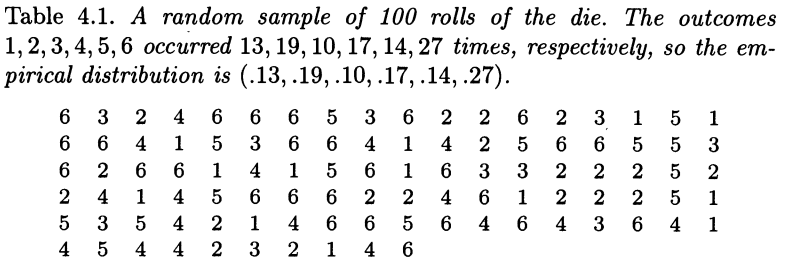
\includegraphics[width=\linewidth]{3/t41.png}
\newline

Рассмотрим выборку юридических вузов размером $n = 15$, показанную в Таблице 3.1 и на правой панели Рисунка 3.1. Эмпирическое распределение $F$ ставит вероятность $1/15$ для каждой из 15 точек данных. Пять из 15 точек лежат в наборе $A = \{(y, z): 0 <y <600,0 <z <3.00\}$, поэтому $\widehat{Prob}\{A\} = 5/15 = 0.333$. Обратите внимание, что мы получаем другую эмпирическую вероятность для набора $\{0 <y <600,0 <z \le 3.00\}$, поскольку одна из 15 точек данных имеет $GPA = 3.00$, $LSAT < 600$. 

Таблица 4.1 показывает случайную выборку из $n = 100$ бросков кубика: $x_1 = 6, x_2 = 3, x_3 = 2,\cdots, x_{100} = 6$. Эмпирическое распределение $F$ ставит вероятность $1/100$ для каждого из 100 исходов. В подобных случаях, когда есть повторяющиеся значения, мы можем более экономично выразить $F$ как вектор наблюдаемых частот $\hat f_k$, $k=1,2,\cdots,6$
\begin{equation}
    \hat f_k = \#\{x_i=k\}/n.
\end{equation}
Для данных в таблице 4.1 $\hat F= (0.13, 0.19, 0.10, 0.17, 0.14, 0.27)$.

Эмпирическое распределение -- это список значений, принимаемых выборкой $x = (x_1, x_2, \cdots, x_n)$, вместе с долей случаев, когда каждое значение встречается. Часто каждое значение, встречающееся в выборке, появляется только один раз, как в случае с данными юридических школ. Повторения, как и в случае с кубиком таблицы 4.1, позволяют сократить список. В любом случае каждой из $n$ точек данных $x_i$ приписывается вероятность $1 / n$ эмпирическим распределением. 

Очевидно ли, что мы не потеряли информацию при переходе от полного набора данных $(x_1, x_2,\cdots, x_{100})$ в таблице 4.1 к сокращенному представлению в терминах частот? Нет, но это правда. Можно доказать, что вектор наблюдаемых частот $\hat F = (\hat f_1, \hat f_2, \cdots)$ является достаточной статистикой для истинного распределения $F = (f_1, f_2, \cdots)$. Это означает, что вся информация о $F$, содержащаяся в $\mathbf{x}$, также содержится в $\hat F$. 
\newline

\noindent
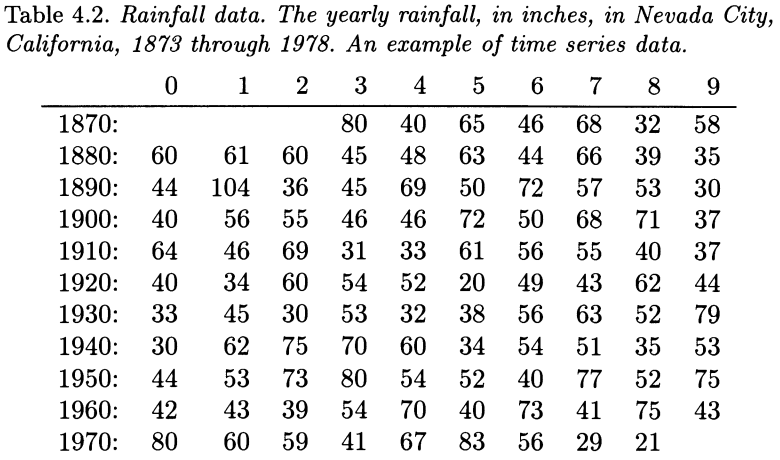
\includegraphics[width=\linewidth]{3/t42.png}
\newline

Теорема достаточности предполагает, что данные были сгенерированы случайной выборкой из некоторого распределения $F$. Это, конечно, не всегда верно. Например, данные о мышах в Таблице 2.1 включают два распределения вероятностей, одно для лечения и одно для контроля. В таблице 4.2 показан временной ряд из 106 чисел: годовое количество осадков в Невада-Сити, Калифорния, с 1873 по 1978 год. Мы могли бы вычислить эмпирическое распределение $F$ для этого набора данных, но оно не будет включать никакой информации временного ряда, например, если большие числа следуют за большими числами. На данный момент мы ограничиваем внимание данными, полученными путем случайной выборки из одного распределения, так называемой ситуации с одной выборкой. Это не так строго, как кажется. Например, в примере с данными о мышах мы можем применить результаты по одной выборке отдельно к экспериментальной и контрольной популяциям. 

При применении статистической теории к реальным задачам ответы на интересующие вопросы обычно формулируются в терминах вероятностных распределений. Мы можем спросить, справедлива ли матрица, дающая данные в Таблице 4.1. Это эквивалентно вопросу, равно ли распределение вероятностей $F$ кубика $(1/6, 1/6, 1/6, 1/6, 1/6, 1/6)$. В примере с юридической школой вопрос может заключаться в том, насколько коррелируют LSAT и GPA. В терминах $F$, распределение $x = (y, z) = (LSAT, GPA)$, это вопрос о значении коэффициента корреляции совокупности
\begin{equation}
    corr(y,z)=\frac{\sum_{j=1}^{82}(Y_j-\mu_y)(Z_j-\mu_z)}{[\sum_{j=1}^{82}(Y_j-\mu_y)^2\sum_{j=1}^{82}(Z_j-\mu_z)^2]^\frac{1}{2}},
\end{equation}
где $(Y_j, Z_j)$ -- j-я точка в популяции юридических школ $\mathbf{X}$, а $\mu_y = \sum_{j=1}^{82} Y_j / 82$, $\mu_z = \sum_{j=1}^{82} Z_j / 82$.

Когда распределение вероятностей $F$ известно (т.е. когда у нас есть полная совокупность $\mathbf{X}$), ответы на такие вопросы требуют не более чем арифметических операций. Для совокупности юридических школ перепись в таблице 3.2 дает $\mu_y = 597.5$, $\mu_z = 3.13$ и 
\begin{equation}
    corr(y,z)=0.761.
\end{equation}
Это первоначальное определение «статистики». Обычно у нас нет генеральной совокупности. Поэтому нам нужен статистический вывод, более современная статистическая теория для вывода свойств $F$ из случайной выборки $\mathbf{x}$. 

Если бы у нас была только выборка юридических школ размером 15, таблица 3.1, мы могли бы оценить $corr (y, z)$ с помощью коэффициента корреляции выборки 
\begin{equation}
    \widehat{corr}(y,z)=\frac{\sum_{j=1}^{15}(y_j-\hat\mu_y)(z_j-\hat\mu_z)}{[\sum_{j=1}^{15}(y_j-\hat\mu_y)^2\sum_{j=1}^{15}(z_j-\hat\mu_z)^2]^\frac{1}{2}},
\end{equation}
где $(y_j, z_j)$ - j-я точка в таблице 3.1, $j = 1, 2, \cdots, 15$ и $\hat\mu_y = \sum_{j=1}^{15}y_j/15$, $\hat\mu_z = \sum_{j=1}^{15}z_j / 15$. Таблица 3.1 дает $\mu_y = 600.3$, $\mu_z = 3.09$ и 
\begin{equation}
    \widehat{corr}(y,z)=0.776.
\end{equation}

Вот еще один пример оценки плагина. Предположим, нас интересует оценка вероятности того, что результат LSAT превышает 600, то есть 
\begin{equation}
    \theta=\frac{1}{82}\sum_1^{82}I_{\{Y_i>600\}}.
\end{equation}
Поскольку 39 из 82 баллов LSAT превышают 600, $\theta = 39/82 = 0.48$. Плагин оценка $\theta$ доли баллов LSAT, превышающих 600, равна 
\begin{equation}
    \hat\theta=\frac{1}{15}\sum_1^{15}I_{\{y_i>600\}}.
\end{equation}
Шесть из 15 баллов LSAT превышают 600, поэтому $\hat\theta = 6/15 = 0.4$. 

Для кубика в Таблице 4.1 у нас нет данных переписи, а есть только выборка $\mathbf{x}$, поэтому на любые вопросы о справедливости кубика необходимо отвечать, исходя из эмпирических частот
\begin{equation}
    \hat F=(\hat f_1, \hat f_2,\cdots,\hat f_6)=(0.13,0.19,0.10,0.17,0.14,0.27).
\end{equation}

Обсуждения статистического вывода сформулированы в терминах параметров и статистики. Параметр -- это функция распределения вероятностей $F$. Статистика -- это функция выборки $\mathbf{x}$. Таким образом, $corr (y, z)$, (4.4), является параметром $F$, а $\widehat{corr} (y, z)$, (4.6), является статистикой, основанной на $\mathbf{x}$. Точно так же $f_k$ -- это параметр $F$, а $\hat f_k$ -- статистика, $k = 1, 2, 3, \cdots, 6$.

Иногда мы будем писать параметры напрямую как функции от $F$, например
\begin{equation}
    \theta=t(F).
\end{equation}
Это обозначение подчеркивает, что значение параметра $\theta$ получается путем применения некоторой процедуры численной оценки $t(\cdot)$ к функции распределения $F$. Например, если $F$ -- это распределение вероятностей на действительной прямой, математическое ожидание можно представить как параметр 
\begin{equation}
    \theta=t(F)=E_F(x).
\end{equation}
Здесь $t(F)$ или $\theta$ вычисляется через математическое ожидание, то есть среднее значение $x$, взвешенное в соответствии с $F$. Для распределения $F$, такого как $F = Bi (n, p)$, мы можем вычислить $t (F) = np$. Даже если $F$ неизвестна, форма $t (F)$ сообщает нам функциональное отображение из $F$ в $\theta$. 
\section{Принцип плагина}

Принцип плагина представляет собой простой метод оценки параметров по выборкам. Плагин оценка параметра $\theta = t (F)$ определяется как 
\begin{equation}
    \hat\theta=t(\hat F).
\end{equation}
Другими словами, мы оцениваем функцию $\theta = t (F)$ распределения вероятностей $F$ той же функцией эмпирического распределения $\hat F$, $\hat\theta = t (\hat F)$. (Статистические данные, подобные (4.13), которые используются для оценки параметров, иногда называют суммарной статистикой, а также оценками и оценщиками.) 

Мы уже использовали принцип плагина при оценке $f_k$ через $\hat f_k$ и при оценке $corr (y, z)$ с помощью $\widehat{corr} (y, z)$. Чтобы убедиться в этом, обратите внимание, что наша совокупность $F$ юридических школ может быть записана как $F = (f_1, f_2,\cdots ,f_82)$, где каждое $f_j$, вероятность j-го юридической школы, имеет значение 1/82. Это распределение вероятностей на $\mathbf{X}$, 82 парах юридических школ. Коэффициент корреляции генеральной совокупности можно записать как 
\begin{equation}
    corr(y,z)=\frac{\sum_{j=1}^{82}f_j(Y_j-\mu_y)(Z_j-\mu_z)}{[\sum_{j=1}^{82}f_j(Y_j-\mu_y)^2\sum_{j=1}^{82}f_j(Z_j-\mu_z)^2]^\frac{1}{2}},
\end{equation}
где
\begin{equation}
    \mu_y=\sum_{j=1}^{82}f_jY_j,\qquad\mu_z=\sum_{j=1}^{82}f_jZ_j.
\end{equation}
Установка каждого $f_j = 1/82$ дает выражение (4.4). Теперь для нашей выборки $(x_1, x_2,\cdots, x_15)$ выборочная частота $\hat f_j$ -- это доля точек выборки, равная $X_j$:
\begin{equation}
    \hat f_j=\#\{x_i=X_j\}/15, j=1,2,\ldots,82.
\end{equation}
Для выборки из Таблицы 3.1 $\hat f_1 = 0, \hat f_2 = 0, \hat f_3 = 0, \hat f_4 = 1/15$ и т.д. Теперь подставив эти значения $\hat f_j$ в выражения (4.15) и (4.14), получим $\hat\mu_y$, $\hat\mu_z$ и $\widehat{corr} (y, z)$ соответственно. То есть $\hat\mu_y$, $\hat\mu_z$ и $\widehat{corr} (y, z)$ -- это плагин оценки $\mu_y$, $\mu_z$ и $corr (y, z)$. 

В общем, плагин оценка математического ожидания $\theta = E_F (x)$ равна 
\begin{equation}
    \hat\theta = E_{\hat F} (x)=\frac{1}{n}\sum_{i=1}^nx_i=\bar x.
\end{equation}

Насколько хорош принцип плагина? Обычно, если единственная доступная информация о $F$ исходит из выборки $\mathbf{x}$, то $\hat\theta = t (\hat F)$ не может быть улучшена как оценка $\theta = t (F)$, по крайней мере, не в обычном асимптотическом ($n\rightarrow\infty$) смысле статистической теории. Например, если $\hat f_k$ -- плагин оценка частоты $\#\{x_i = k\} / n$, то 
\begin{equation}
    \hat f_k\sim Bi(n,f_k)/n.
\end{equation}
В этом случае оценка $\hat f_k$ является несмещенной для $f_k$, $E(\hat f_k) = f_k$, с дисперсией $f_k (1-f_k) / n$. Это наименьшая возможная дисперсия для несмещенной оценки $f_k$. 

Мы будем использовать бутстреп для изучения смещения и стандартной ошибки плагин оценки $\hat\theta = t (\hat F)$. Достоинство бутстрепа состоит в том, что он автоматически создает смещения и стандартные ошибки, независимо от того, насколько сложным может быть функциональное сопоставление $\theta = t (F)$. Мы увидим, что сам бутстреп является применением плагин принципа. 

Принцип плагина менее эффективен в ситуациях, когда имеется информация о $F$, отличная от той, которая предоставлена выборкой $\mathbf{x}$. Мы можем знать или предполагать, что $F$ является членом параметрического семейства, например семейства многомерных нормальных распределений. Или мы можем оказаться в ситуации регрессии, когда у нас есть набор случайных выборок $\mathbf{x} (z)$ в зависимости от переменной-предиктора $z$. Тогда, даже если нас интересует только $F_{z_0}$, функция распределения для некоторого конкретного значения $z_o$ из $z$, может быть информация о $F_{z_o}$ в других выборках $\mathbf{x} (z)$, особенно тех, для которых $z$ близок к $z_0$.

Принцип плагина и бутстреп могут быть адаптированы к параметрическим семействам и регрессионным моделям. В следующих нескольких главах мы предполагаем, что находимся в ситуации, когда у нас есть только одна случайная выборка $\mathbf{x}$ из полностью неизвестного распределения $F$. Это называется непараметрической задачей с одной выборкой.

\chapter{Стандартные ошибки и оценки стандартных ошибок}
\section{Введение}

Сводная статистика, такая как $\hat\theta = t (\hat F)$, часто является первым результатом анализа данных. Следующее, что мы хотим знать -- это точность $\hat\theta$. Бутстреп обеспечивает оценки точности, используя принцип плагина для оценки стандартной ошибки сводной статистики. Это предмет следующей главы. Сначала мы обсудим оценку стандартной ошибки среднего, где принцип плагина может быть реализован явно. 
\section{Стандартная ошибка среднего}

Предположим, что $x$ -- вещественная случайная величина с распределением вероятностей $F$. Обозначим математическое ожидание и дисперсию $F$ символами $\mu_F$ и $\sigma^2_F$ соответственно,
\begin{equation}
    \mu_F=E_F(x),\qquad \sigma^2_F=var_F(x)=E_F[(x-\mu_F)^2].
\end{equation}
В главе 3 эти величины назывались $\mu_x$ и $\sigma^2_x$. Здесь мы подчеркиваем зависимость от $F$. Альтернативное обозначение $var_F (x)$ для дисперсии, иногда сокращенное до $var (x)$, означает то же самое, что и $\sigma^2_F$. В дальнейшем мы иногда будем писать
\begin{equation}
    x\sim(\mu_F,\sigma^2_F)
\end{equation}
чтобы кратко обозначить математическоу ожидание и дисперсию $x$.

Теперь пусть $(x_1,\cdots, x_n)$ будет случайной выборкой размера $n$ из распределения $F$. Среднее значение выборки $\bar x = \sum_{i=1}^n x_i / n$ имеет математическое ожидание $\mu_F$ и дисперсию $\sigma^2_F/n$, 
\begin{equation}
    \bar x\sim(\mu_F,\sigma^2_F/n).
\end{equation}
Другими словами, математическоу ожидание $\bar x$ такое же, как ожидание одного $x$, но дисперсия $\bar x$ равна $1 / n$ дисперсии $x$. Это причина использования средних значений: чем больше $n$, тем меньше $var (\bar x)$, поэтому большее $n$ означает лучшую оценку $\mu_F$·

Стандартная ошибка среднего $\bar x$, записанная как $se_F (\bar x)$ или $se (\bar x)$, является квадратным корнем из дисперсии $\bar x$, 
\begin{equation}
    se_F (\bar x) = [var_F(\bar x)]^{1/2} = \sigma_F/\sqrt{n}.
\end{equation}
Стандартная ошибка -- это общий термин для стандартного отклонения сводной статистики. Это наиболее распространенный способ индикации статистической точности. Грубо говоря, мы ожидаем, что $|\bar x-\mu_F|$ будет меньше одной стандартной ошибки примерно в 68\% случаев и меньше двух стандартных ошибок примерно в 95\% случаев. 

Эти проценты основаны на центральной предельной теореме. При довольно общих условиях на $F$ распределение $\bar x$ будет приблизительно нормальным при увеличении $n$, что мы можем записать как 
\begin{equation}
    \bar x\sim N(\mu_F,\sigma^2_F/n).
\end{equation}
Математическое ожидание $\mu_F$ и дисперсия $\sigma^2_F/n$ в (5.5) точны, только нормальность является приблизительной. Используя (5.5), таблица нормального распределения дает 
\begin{equation}
    Prob\{|\bar x - \mu_F|<\frac{\sigma_F}{\sqrt{n}}\}=0.683\qquad Prob\{|\bar x - \mu_F|<\frac{2\sigma_F}{\sqrt{n}}\}=0.954,
\end{equation}
как показано на Рисунке 5.1. Одно из преимуществ бутстрепа заключается в том, что не нужно полностью полагаться на центральную предельную теорему.
\newline

\noindent
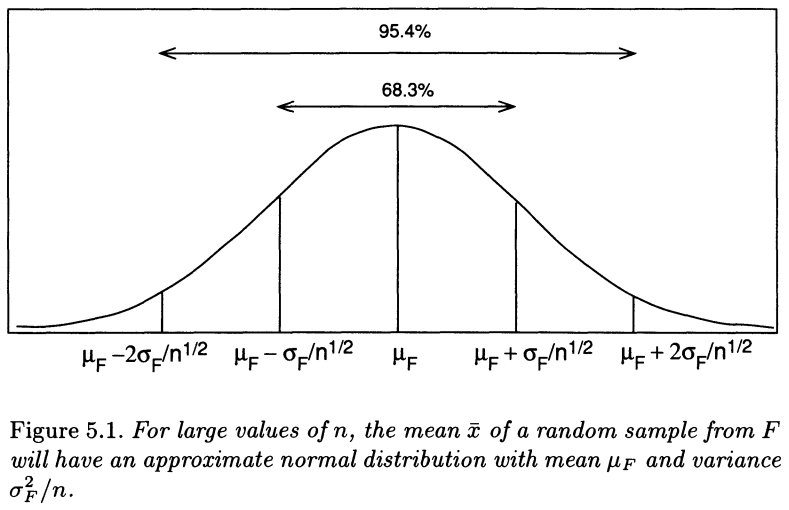
\includegraphics[width=\linewidth]{4/f51.png}
\newline
Простой пример показывает ограничения аппроксимации центральной предельной теоремы. Предположим, что $F$ -- это распределение, которое ставит вероятность только для двух исходов, 0 или 1, скажем 
\begin{equation}
    Prob\{x=1\}=p\qquad Prob\{x=0\}=1-p.
\end{equation}
Здесь $p$ -- параметр $F$, часто называемый вероятностью успеха, имеющий значение от 0 до 1. Случайная выборка $F \rightarrow (x_1, x_2,\cdots, x_n)$ может рассматриваться как $n$ независимых подбрасываний монеты с вероятностью успеха (или «орла», или $x = 1$) равной $p$. Тогда сумма $s = \sum_{i=1}^nx_i$ -- количество успехов в $n$ независимых бросках монеты; $s$ имеет биномиальное распределение (3.3), 
\begin{equation}
    s\sim Bi(n,p).
\end{equation}
Среднее значение $\bar x = s / n$ равно $\hat p$ в плагин оценке $p$ Распределение (5.7) имеет $\mu_F=p$, $\sigma^2_F = p (1- p)$, поэтому (5.3) дает 
\begin{equation}
    \hat p\sim (p,p(1-p)/n)
\end{equation}

для среднего и дисперсии $\hat p$ Другими словами, $\hat p$ -- это несмещенная оценка $p$, $E (\hat p) = p$, со стандартной ошибкой 
\begin{equation}
    se(\hat p)=\left[\frac{p(1-p)}{n}\right]^{1/2}.
\end{equation}
\newline

\noindent
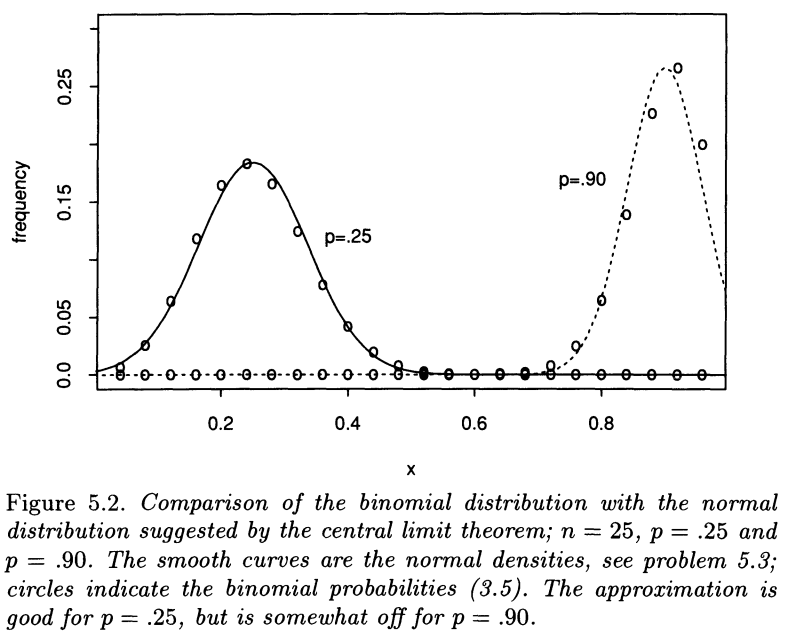
\includegraphics[width=\linewidth]{4/f52.png}
\newline
На рис. 5.2 показана центральная предельная теорема, работающая для биномиального распределения при $n = 25$, $p = 0.25$ и $p = 0.90$. Центральная предельная теорема дает хорошее приближение к биномиальному распределению для $n = 25$, $p = 0.25$, но несколько хуже для $n = 25$, $p = 0.9$. 
\section{Оценка стандартной ошибки среднего}

Предположим, что у нас есть случайная выборка чисел $F \rightarrow x_1, x_2, \cdots, x_n$, например контрольные измерения $n = 9$ для данных о мышах из таблицы 2.1. Мы вычисляем оценку $\bar x$ для математического ожидания $\mu_F$, равного 56.22 для данных о мышах, и хотим знать стандартную ошибку $\bar x$. Формула (5.4) $se_F (\bar x) = \sigma_F/\sqrt{n}$ включает неизвестное распределение $F$ и поэтому не может использоваться напрямую. 

На этом этапе мы можем использовать принцип плагина: мы подставляем $\hat F$ вместо $F$ в формуле $se_F (\bar x) = \sigma_F/\sqrt{n}$. Плагин оценка $\sigma_F = [E_F (x- \mu_F)^2]^{1/2}$ равна
\begin{equation}
    \hat\sigma=\sigma_{\hat F}=\{\frac{1}{n}\sum_{i=1}^n(x_i-\bar x)^2\}^{1/2},
\end{equation}
поскольку $\mu_{\hat F}= \bar x$ и $E_{\hat F}g (x) = \frac{1}{n}\sum_{i=1}^n g (x_i)$ для любой функции $g$. Это дает оценку стандартной ошибки $\widehat{se} (\bar x) = se_{\hat F} (\bar x)$, 
\begin{equation}
    \widehat{se} (\bar x) = \sigma_{\hat F}/\sqrt{n}=\{\sum_{i=1}^n(x_i-\bar x)^2/n^2\}^{1/2}.
\end{equation}
Для контрольной группы данных о мышах $\widehat{se} (\bar x) = 13.33$.

Формула (5.12) немного отличается от обычной оценки стандартной ошибки (2.2). Это потому, что $\sigma_F$ обычно оценивается как $\bar\sigma=\{\sum(x_i-\bar x)^2/(n-1)\}^{1/2}$, а не как $\hat\sigma$, (5.11). Деление на $n - 1$ вместо $n$ делает $\bar\sigma^2$ несмещенной для $\sigma_F^2$. Для большинства целей $\hat\sigma$ так же хороша, как $\bar\sigma$ для оценки $\sigma_F$. 

Обратите внимание, что мы использовали принцип плагина дважды: сначала для оценки математического ожидания $\mu_F$ с помощью $\mu_{\hat F} = \bar x$, а затем для оценки стандартной ошибки $se_F (\bar x)$ с помощью $se_{\hat F} (\bar x)$. Бутстреп оценка стандартной ошибки, о которой идет речь в главе 6, сводится к использованию принципа плагина для оценки стандартной ошибки произвольной статистики $\hat\theta$. Здесь мы видели, что если $\hat\theta = \bar x$, то этот подход приводит к (почти) обычной оценке стандартной ошибки. Как мы увидим, преимущество бутстрепа в том, что его можно применить практически к любой статистике $\hat\theta$, а не только к среднему значению $\bar x$. 

\chapter{Бутстреп оценка стандартной ошибки}
\section{Введение}

Предположим, мы находимся в следующей общей ситуации анализа данных: была обнаружена случайная выборка $\mathbf{x} = (x_1, x_2, \cdots, x_n)$ из неизвестного распределения вероятностей $F$, и мы хотим оценить интересующий параметр $\theta = t (F)$ на основе $\mathbf{x}$. Для этого мы вычисляем оценку $\hat\theta = s (\mathbf{x})$ из $\mathbf{x}$. [Обратите внимание, что $s (\mathbf{x})$ может быть плагин оценкой $t (\hat F)$, но это не обязательно.] Насколько точна $\hat\theta$? Бутстреп был представлен в 1979 году как компьютерный метод оценки стандартной ошибки $\hat\theta$. Он имеет то преимущество, что он полностью автоматический. Самостоятельная оценка стандартной ошибки не требует теоретических вычислений и доступна независимо от того, насколько математически сложной может быть оценка $\hat\theta = s (\mathbf{x})$. Это описано и проиллюстрировано в этой главе. 
\section{Бутстреп оценка стандартной ошибки}

Бутстреп методы зависят от понятия бутстреп выборки. Пусть $\hat F$ -- эмпирическое распределение, присваивающее вероятность $1 / n$ на каждое из наблюдаемых значений $x_i$, $i = 1, 2,\cdots, n$, как описано в главе 4. Бутстреп выборка является случайной выборкой размера $n$, набранной из $\hat F$, скажем, $\mathbf{x}^* = (x_1^*, x_2^*, \cdots, x_n^*)$,
\begin{equation}
    \hat F\rightarrow (x_1^*, x_2^*, \cdots, x_n^*).
\end{equation}
<<*>> указывает, что $\mathbf{x}^*$ не является фактическим набором данных $\mathbf{x}$, а скорее рандомизированной или перезапущенной версией $\mathbf{x}$.

Есть еще один способ сказать (6.1): точки бутстреп данных $x_1^*, x_2^*, \cdots, x_n^*$ являются случайной выборкой размера $n$, выбранной с заменой из совокупности $n$ объектов $(x_1, x_2, \cdots, x_n )$. Таким образом, мы могли бы иметь $x_1^* = x_7, x_2^* = x_3, x_4^* = x_3, x_4^* = x_{22},\cdots, x_n^* = x_7$. Набор бутстреп данных $(x_1^*, x_2^*, \cdots, x_n^*)$ состоит из элементов исходного набора данных $(x_1, x_2,\cdots, x_n)$, некоторые из которых появляются ноль раз, некоторые появляются один раз, некоторые появляются дважды, и так далее.

В соответствии с набором бутстреп данных $\mathbf{x}^*$, бутстреп репликация $\hat\theta$ -- это
\begin{equation}
    \hat\theta^*=s(\mathbf{x}^*).
\end{equation}
Величина $s(\mathbf{x}^*)$ является результатом применения той же функции $s (\cdot)$ к $\mathbf{x}^*$, которая была применена к $\mathbf{x}$. Например, если $s(\mathbf{x})$ является выборочным средним значением $\bar x$, то $s(\mathbf{x}^*)$ -- это среднее значение набора бутстреп данных, $\bar x^*=\sum_{i=1}^nx_i^*/n$. 

Бутстреп оценка $se_F (\hat\theta)$ стандартной ошибки статистики $\hat\theta$ представляет собой плагин оценку, которая использует эмпирическую функцию распространения $\hat F$ вместо неизвестного распределения $F$. В частности, бутстреп оценка  $se_F (\hat\theta)$ определяется, как 
\begin{equation}
    se_{\hat F} (\hat\theta^*).
\end{equation}
Другими словами, бутстреп оценка $se_F (\hat\theta)$ является стандартной ошибкой $\hat\theta$ для наборов данных размером $n$, случайным образом выбранных из $\hat F$. 

Формула (6.3) называется идеальной бутстреп оценкой ошибки $\hat\theta$. К сожалению, для практически любой оценки $\hat\theta$, кроме среднего, нет точной формулы (5.4), которая позволяет вычислить числовое значение идеальной оценки точно. Бутстреп алгоритм, описанный ниже, является вычислительным способом получения хорошего приближения к численному значению $se_{\hat F} (\hat\theta^*)$. 

Легко реализовать бутстреп выборку на компьютере. Устройство выбирает случайные целые числа $i_1, i_2, \cdots, i_n$, каждое из которых равняется любому значению между 1 и $n$ с вероятностью $1 / n$. Бутстреп выборка состоит из соответствующих членов $\mathbf{x}$,
\begin{equation}
    x_1^*=x_{i_1},x_2^*=x_{i_2},\cdots,x_n^*=x_{i_n}.
\end{equation}

Бутстреп алгоритм работает путем выбора множества независимых бутстреп выборок, оценки соответствующих бутстреп репликаций и оценки стандартной ошибки $\hat\theta$ через эмпирическое стандартное отклонения репликаций. Результат называется бутстреп оценкой стандартной ошибки, обозначенной $\widehat{se}_B$, где $B$ -- количество используемых бутстреп выборок.

Алгоритм 6.1 -- это более явное описание бустреп процедуры для оценки стандартной ошибки $\hat\theta=s(\mathbf{x})$ из наблюдаемых данных $\mathbf{x}$. 

\newpage
\begin{center}
    \textit{Алгоритм 6.1}
    
    \underline{Бутстреп алгоритм для оценки стандартных ошибок}
    
    \begin{enumerate}
        \item Выберите $B$ независимых бутстреп выборок $x^{*1}, x^{*2},\cdots, x^{*B}$, каждый из которых состоит из $n$ точек данных, выбранных с заменой их $\mathbf{x}$, как в (6.1) или (6.4). [Для оценки стандартной ошибки B обычно будет в диапазоне 25-200, см. Таблицу 6.1.] 
        
        \item Оцените бутстреп репликацию, соответствующую каждой бутстреп выборке,
        \begin{equation}
            \hat\theta^*(b)=s(\mathbf{x}^{*b})\qquad b=1,2,\cdots,B.
        \end{equation}
        
        \item Оцените стандартную ошибку $se_F (\hat\theta)$ через выборочное стандартное отклонение $B$ репликаций 
        \begin{equation}
            \widehat{se}_B=\left\{\sum_{b=1}^B[\hat\theta^*(b)-\hat\theta^*(\cdot)]^2/(B-1)\right\}^{1/2},
        \end{equation}
        где $\hat\theta^*(\cdot)=\sum_{b=1}^B\hat\theta^*(b)/B$.
    \end{enumerate}
\end{center}

На рисунке 6.1 изображена схематическая диаграмма бутстреп алгоритма стандартных ошибок. 

Предел $\widehat{se}_B$ по $B$ стремится к бесконечности -- это идеальная бутстреп оценка $se_F(\hat\theta)$,
\begin{equation}
    \lim_{B\rightarrow\infty}\widehat{se}_B=se_{\hat F}=se_{\hat F}(\hat\theta^*).
\end{equation}
Тот факт, что $\widehat{se}_B$ стремится к $se_{\hat F}$ при $B$, стремящимся к бесконечности, позволяет сказать, что эмпирическое стандартное отклонение приближается к стандартному отклонению совокупности с увеличением количества репликаций. «Совокупность» в этом случае является совокупностью значений $\hat\theta^*=s(\mathbf{x}^*)$, где $\hat F \rightarrow (x_1^*, x_2^*, \cdots, x_n^*) = \mathbf{x}^*$. 

Идеальная бутстреп оценка $se_{\hat F}\hat\theta^*$ и его приближение $\widehat{se}_B$ иногда называют непараметрическими бутстреп оценками, потому что они основаны на $\hat F$, непараметрической оценке $F$. В разделе 6.5 мы обсуждим параметрический бутстреп, который использует другую оценку F. 

Немного об обозначениях: в (6.7) мы пишем $se_{\hat F}(\hat\theta^*)$, а не $se_{\hat F}(\hat\theta)$, чтобы избежать путаницы между $\hat\theta$, значением $s (\mathbf{x})$ на основе наблюдаемых данных, и $\hat\theta^* = s (\mathbf{x}^*)$, случайной величиной на основе бутстреп выборки. Более подробное обозначение $se_{\hat F} (\hat\theta (\mathbf{x}^*))$ подчеркивает, что $se_{\hat F}$ является бутстрепированной стандартной ошибкой: фактические данные $\mathbf{x}$ остаются фиксированным в (6.7); Случайность в расчете исходит из изменчивости бутстреп выборок $\mathbf{x}^*$ для данного x. Точно так же мы будем писать $E_{\hat F}g(\mathbf{x^*})$, чтобы указать бутстрепированное математическое ожидание функции $g (\mathbf{x}^*)$: математическое ожидание с фиксированным $\mathbf{x}$ (и $\hat F$) и случайным $\mathbf{x}^*$ в соответствии с (6.1). 
\newline

\noindent
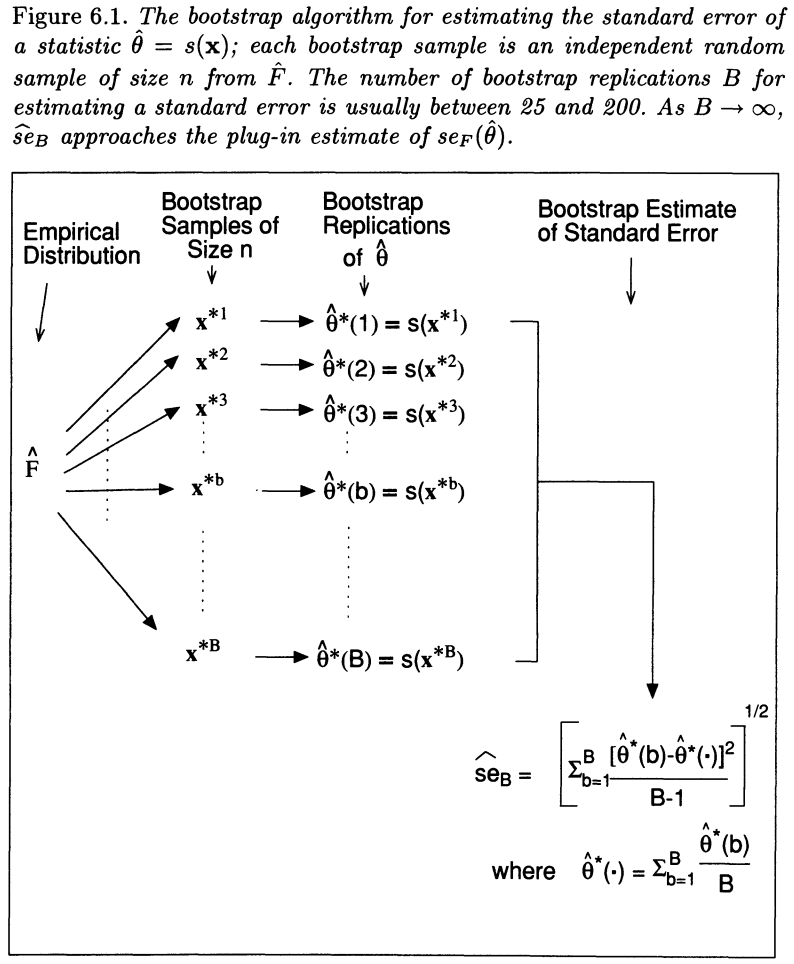
\includegraphics[width=\linewidth]{5/f61.png}
\newline

Всего существует $C_n^{2n-1}$ различных бутстреп выборок. Обозначим их через $z^1, z^2, \ldots z^m$, где $m = C_n^{2n-1}$. Например, если $n = 2$, отдельными выборками являются $(x_1, x_1)$, $(x_2, x_2)$ и $(x_1, x_2)$; поскольку порядок не имеет значения, $(x_2, x_1)$ совпадает с $(x_1, x_2)$. Вероятность получения одной из этих выборок при выборе с заменой может быть получена из полиномиального распределения. Обозначим вероятность $j$-й выборки через $\omega_j, j = 1, 2, \ldots C_n^{2n-1}$. Тогда прямым способом вычисления идеальной бутстреп оценки стандартной ошибки будет использование стандартного отклонения совокупности m бутстреп значений $s (z^j)$:
\begin{equation}
    se_{\hat F}(\hat\theta^*)=[\sum_{j=1}^m\omega_j\{s(z^j)-s(\cdot)\}^2]^{1/2}
\end{equation}
где $s (\cdot) = \sum_{j=1}^m\omega_js(z^j)$. Сложность этого подхода заключается в том, что, если $n$ не достаточно мало $(\le 5)$, число $C_n^{2n-1}$ очень велико, что делает вычисление (6.8) непрактичным. Отсюда необходимость в бутстрап выборкaх, описаных выше. 
\section{Пример: коэффициент корреляции}

Мы уже видели два примера бутстреп оценок стандартной ошибки для среднего и медианного значения для экспериментальной группы данных о мышах, таблица 2.1. В качестве второго примера рассмотрим выборочный коэффициент корреляции между $y = LSAT$ и $z = GPA$ для $n = 15$ точек данных о юридических школах, таблица 3.1, $\widehat{corr}(y, z) =0.776$. Насколько точна оценка $0.776$? В таблице 6.1 показана бутстреп оценка стандартной ошибки $\widehat{se}_B$ для $B$ в диапазоне от $25$ до $3200$. Последнее значение, $\widehat{se}_{3200} = 0.132$, является нашей оценкой $se_F (\widehat{corr})$. Позже мы увидим, что $\widehat{se}_{200}$ почти так же хороша для оценки $se_F$, как $\widehat{se}_{3200}$· 

Глядя на правую часть рисунка 3.1, читатель может представить себе, как работает генерация бутстреп выборок. Выборочная корреляция по $n = 15$ исходным точкам данных составляет $\widehat{corr} = 0.776$. Бутстреп выборка состоит из $15$ точек, выбранных случайным образом и заменяющих исходные $15$. Корреляция бутстреп выборки представляет собой бутстреп репликацию $\widehat{corr}^*$, которая может быть больше или меньше, чем $\widehat{corr}$. Независимые повторения генерации бутстреп выборок дают бутстреп репликации $\widehat{corr}^*(1),\widehat{corr}^*(2),\cdots,\widehat{corr}^*(B)$. Наконец, $\widehat{se}_B$ -- выборочное стандартное отклонение значений $\widehat{corr}^*(b)$. 
\newline

\noindent
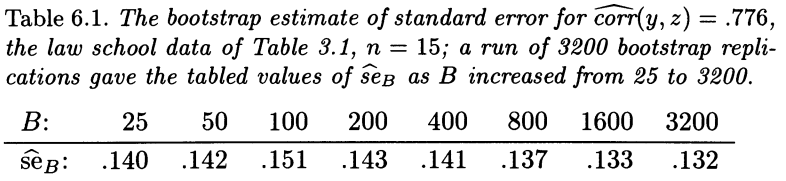
\includegraphics[width=\linewidth]{5/t61.png}
\newline

Левая панель рисунка 6.2 представляет собой гистограмму $3200$ бутстреп репликаций $\widehat{corr}^*(b)$. Всегда рекомендуется просматривать бутстреп данные графически, а не полагаться полностью на одну сводную статистику, такую как $\widehat{se}_B$. В примере корреляции может оказаться, что несколько выпадающих значений $\widehat{corr}^*(b)$ сильно раздувают $\widehat{se}_B$, и в этом случае стоит использовать более надежную меру стандартного отклонения; Выводы, основанные на нормальной кривой, как в (5.6) и на рисунке 5.1, сомнительны, когда бутстреп гистограмма явно ненормальна.

В примере с юридическими школами у нас есть полная совокупность $\mathbf{X}$ из $N = 82$ школ, Таблица 3.2. В правой части рисунка 6.2 показана гистограмма $\widehat{corr} (y, z)$ для $3200$ выборок размера $n = 15$, взятых из $\mathbf{X}$. Другими словами, $3200$ случайных выборок $\mathbf{x} = (x_1, x_2, \cdots, x_{15})$ были составлены с заменой из $82$ точек в $\mathbf{X}$, и $\widehat{corr}(\mathbf{x})$ оценивался для каждого из них. Стандартное отклонение $3200$ значений $\widehat{corr}(\mathbf{x})$ составило $0.131$, таким образом $\widehat{se}_B$ является хорошей оценкой стандартной ошибки генеральной совокупности. Что еще более впечатляюще, бутстреп гистограмма слева сильно напоминает гистограмму справа. Помните, что в реальной проблеме у нас была бы только информация слева, из которой мы пытались бы вывести ситуацию справа. 
\newline

\noindent
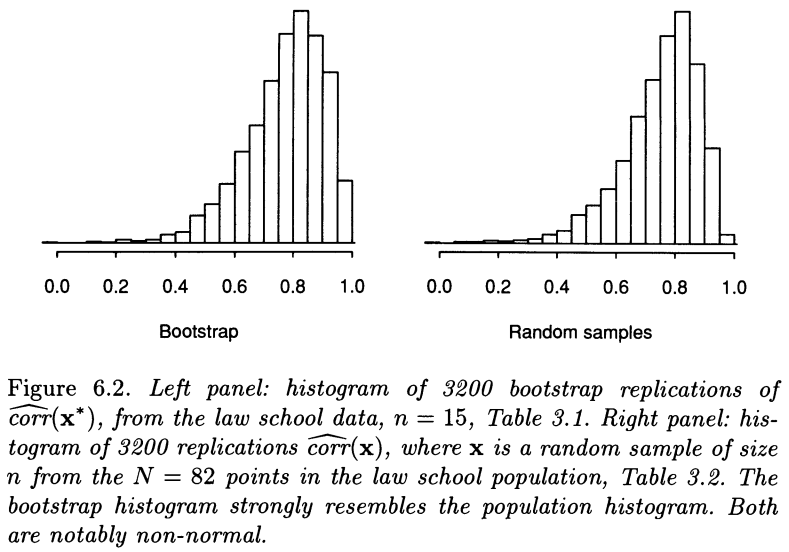
\includegraphics[width=\linewidth]{5/f62.png}
\newline
\section{Количество бутстреп репликаций $B$}

Насколько большим мы должны взять $B$, количество бутстреп репликаций, используемых для оценки $\widehat{se}_B$? Идеальная бутстреп оценка $\widehat{se}_\infty$ использует $B=\infty$, и в этом случае $\widehat{se}_\infty$ равно плагин оценке $se_{\hat F}(\hat\theta^*)$. Формула (5.12) дает $\widehat{se}_\infty$ для $\hat\theta=\bar x$, но для большинства других статистических данных мы должны фактически выполнить генерацию бутстреп выборок. Время, затрачиваемое компьютером, которое в основном зависит от того, сколько времени требуется для оценки бутстреп репликаций (6.5), линейно увеличивается с $B$. Временные ограничения могут диктовать небольшое значение $B$, если $\hat\theta = s (\mathbf{x})$ -- очень сложная функция.

Нам нужно такое же хорошее поведение от оценки стандартной ошибки, что и от оценки любой другой интересующей величины: небольшая систематическая ошибка и небольшое стандартное отклонение. Бутстреп оценка стандартной ошибки обычно имеет относительно небольшое смещение. Идеальная начальная оценка $\widehat{se}_\infty$ имеет наименьшее возможное стандартное отклонение среди почти несмещенных оценок $se_F(\hat\theta)$, по крайней мере, в асимптотическом $(n \rightarrow\infty)$ смысле. Эти хорошие свойства вытекают из того факта, что $\widehat{se}_\infty$ -- это плагин оценка $se_{\hat F}(\hat\theta)^*$. Нетрудно показать, что $\widehat{se}_B$ всегда имеет большее стандартное отклонение, чем $\widehat{se}_\infty$. Практический вопрос: насколько большее?

Приблизительный, но вполне удовлетворительный ответ можно сформулировать в терминах коэффициента вариации $\widehat{se}_B$, отношения стандартного отклонения $\widehat{se}_B$ к его математическому ожиданию. Повышенная изменчивость из-за остановки после $B$ бутстреп репликаций, а не бесконечности, отражается в увеличенном коэффициенте вариации,
\begin{equation}
    cv(\widehat{se}_B)=\left\{cv(\widehat{se}_\infty)^2+\frac{E(\Delta)+2}{4B}\right\}^{1/2}.
\end{equation}
Здесь $\Delta$ -- параметр, который измеряет, насколько длиннохвостым является распределение $\hat\theta^*$: если $\Delta$ равно нулю для нормального распределения, оно колеблется от $-2$ для короткохвостых распределений до произвольно больших значений, когда F длиннохвостное. На практике $\delta$ обычно не превышает $10$. Коэффициент вариации в уравнении (6.9) относится к вариации как на уровне повторных выборок (бутстреп), так и на уровне исходной выборки. Идеальная оценка $\widehat{se}_\infty = se_{\hat F}(\hat\theta^*)$ не идеальна. Она все еще может иметь значительную изменчивость в качестве оценки $se_F(\hat\theta)$ из-за изменчивости $\hat F$ как оценки $F$. Например, если $x_1, x_2, \cdots, x_n$ является случайной выборкой из нормального распределения и $\hat\theta=\bar x$, тогда $cv(\widehat{se}_\infty)=1/\sqrt{2n}$, равное $0.22$ для n = 10. Формула (6.9) имеет важное практическое следствие: для значений $cv(\widehat{se}_\infty)$ и $\Delta$, которые могут возникнуть на практике, $cv(\widehat{se}_B)$ не намного больше, чем $cv(\widehat{se}_\infty)$ для $B\ge 200$. 

Таблица 6.2 сравнивает $cv(\widehat{se}_B)$ с $cv(\widehat{se}_\infty)$ для различных вариантов $B$, предполагая $\Delta = 0$. Очень часто можно ожидать, что $cv(\widehat{se}_\infty)$ будет не меньше, чем $0.10$, и в этом случае $B = 100$ дает вполне удовлетворительные результаты.
\newline

\noindent
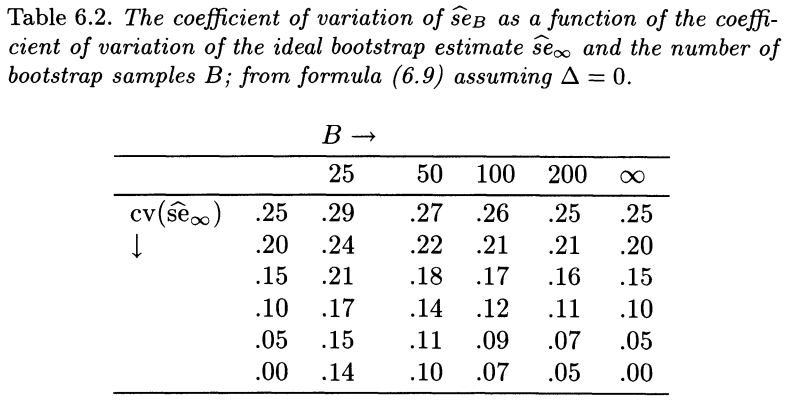
\includegraphics[width=\linewidth]{5/t62.png}
\newline
Вот два практических правила, взятых из опыта:
\begin{enumerate}
    \item Даже небольшое количество бутстреп репликаций, скажем, $B = 25$, обычно является информативным. $B = 50$ часто бывает достаточно, чтобы дать хорошую оценку $se_F (\hat\theta)$.
    \item Очень редко для оценки стандартной ошибки требуется более $B = 200$ репликаций. (Для доверительных бутстреп интервалов требуются гораздо большие значения $B$.) 
\end{enumerate}

Аппроксимации, полученные путем случайной выборки или моделирования, называются оценками Монте-Карло. Вычислительные методы, отличные от прямого моделирования Монте-Карло, иногда могут во много раз сократить количество повторений $B$, необходимых для достижения заданной точности. Между тем стоит помнить, что бутстреп данные, как и реальные данные, заслуживают внимательного изучения. В частности, отображение гистограммы бутстреп репликаций почти никогда не бывает пустой тратой времени. 
\section{Параметрический бутстреп}

Может показаться странным использование бутстреп алгоритма для оценки стандартных ошибок, когда можно использовать формулу из учебника. Фактически, бутстреп выборки могут генерироваться параметрически, в этом случае результаты тесно связаны с формулами стандартных ошибок из учебников. 

Параметрическая бутстреп оценка стандартной ошибки определяется как 
\begin{equation}
    se_{\hat F_{par}}(\hat\theta^*),
\end{equation}
где $\hat F_{par}$ -- оценка $F$, полученная из параметрической модели данных. Здесь мы приведем простой пример, чтобы проиллюстрировать идею. Для данных о юридических школах, вместо оценки $F$ эмпирическим распределением $\hat F$, мы могли бы предположить, что популяция имеет двумерное нормальное распределение. Разумные оценки среднего значения и ковариации этой совокупности даны как $(\bar y, \bar z)$ и
\begin{equation}
    \frac{1}{14}\left(
    \begin{array}{cc}
        \sum(y_i-\bar y)^2 & \sum(y_i-\bar y)(z_i-\bar z) \\
        \sum(y_i-\bar y)(z_i-\bar z) & \sum(z_i-\bar z)^2
    \end{array}
    \right).
\end{equation}
Обозначим двумерную нормальную популяцию с этим средним значением и ковариацией как $\hat F_{norm}$; это пример параметрической оценки совокупности $F$. Используя это, параметрическая бутстреп оценка стандартной ошибки корреляции $\hat\theta$ является $se_{\hat F_{norm}} (\hat\theta^*)$. Как и в непараметрическом случае, идеальная параметрическая бутстреп оценка не может быть легко вычислена, за исключением тех случаев, когда $\hat\theta$ является средним. Поэтому мы аппроксимируем идеальную бутстреп оценку с помощью бутстреп выборок, но другим способом, чем раньше. Вместо выборок с заменой из исходных данных мы берем $B$ выборок размера $n$ из параметрической оценки генеральной совокупности $\hat F_{par}$:
\begin{equation}
    \hat F_{par}\rightarrow(x_1^*,x_2^*,\ldots,x_n^*).
\end{equation}
После генерации бутстреп выборок мы действуем точно так же, как в шагах 2 и 3 бутстреп алгоритма из раздела 6.2: мы оцениваем нашу статистику для каждой бутстреп выборки, а затем вычисляем стандартное отклонение $B$ бутстреп репликаций.

В примере с коэффициентом корреляции, предполагая двумерную нормальную совокупность, мы берем $B$ выборок размером $15$ из $\hat F_{norm}$ и вычисляем коэффициент корреляции для каждой бутстреп выборки. На левой панели рисунка 6.3 показана гистограмма для $B = 3200$ бутстреп репликаций, полученных таким образом. Это очень похоже на гистограммы на рисунке 6.2. Параметрическая бутстреп оценка стандартной ошибки для этих повторений была $0.124$, что близко к значению $0.131$, полученному на непараметрических бутстреп выборках.

Учебная формула для стандартной ошибки коэффициента корреляции составляет $(1-\hat\theta^2) / \sqrt{n- 3}$. Подставляя $\hat\theta = 0.776$, она дает значение $0.15$ для данных о юридических школах.
\newline

\noindent
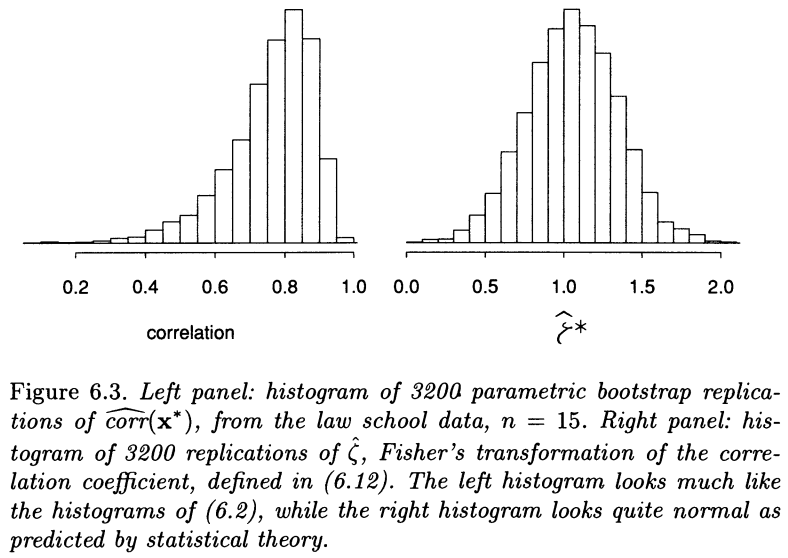
\includegraphics[width=\linewidth]{5/f63.png}
\newline
Мы можем провести дальнейшее сравнение с нашим параметрическим бутстреп результатом. Учебные материалы также утверждают, что преобразование Фишера, примененное к $\hat\theta$
\begin{equation}
    \hat\zeta=0.5\log\left(\frac{1+\hat\theta}{1-\hat\theta}\right)
\end{equation}
приблизительно нормально распределено со средним $\zeta= 0.5  \log\left(\frac{1+\theta}{1-\theta}\right)$ и стандартным отклонением $1 / \sqrt{n-3}$, где $\theta$ является коэффициентом корреляции совокупности. Исходя из этого, обычно выполняется вывод для $\zeta$ и затем преобразуется обратно, чтобы сделать вывод о коэффициенте корреляции. Чтобы сравнить это с нашим параметрическим бутстреп анализом, мы вычислили $\hat\zeta$ вместо $\hat\theta$ для каждой из наших $3200$ бутстреп выборок. Гистограмма значений $\hat\zeta^*$ показана на правой панели рисунка 6.3 и выглядит вполне нормально. Кроме того, стандартное отклонение $3200$ значений $\hat\zeta^*$ было $0.290$, что очень близко к значению $1 / \sqrt{15-3} = 0.289$. 

Это соглашение выполняется в целом. Большинство формул для стандартных ошибок в учебниках являются приближениями, основанными на нормальной теории, и обычно дают ответы, близкие к параметрическому бутстрепу, который отбирает выборки из нормального распределения. Взаимосвязь между бутстрепом и традиционной статистической теорией -- более сложная математическая тема.

У бутстрепа есть два несколько отличных друг от друга преимущества по сравнению с традиционными методами из учебников: 1) при использовании в непараметрическом режиме он избавляет аналитика от необходимости делать параметрические предположения о форме базовой совокупности, и 2) при использовании в параметрическом режиме он обеспечивает болле точные ответы, чем формулы из учебника, и могут дать ответы на задачи, для которых не существует формул из учебника. 

Большая часть этого пособия сосредоточена на непараметрическом применении бутстрепа. Параметрический бутстреп полезен в задачах, где доступны некоторые знания о форме генеральной совокупности, а также для сравнение с непараметрическим анализом. Однако основная причина использования параметрических допущений в традиционном статистическом анализе состоит в том, чтобы облегчить вывод формул для стандартных ошибок из учебников. Поскольку нам не нужны формулы в бутстреп подходе, мы можем избежать ограничительных параметрических предположений. 


\chapter{Бутстреп и стандартные ошибки: некоторые примеры}
\section{Введение}

До внедрения компьютеров вычисляли стандартные ошибки используя методы математического анализа и предположения о распределении, что часто предполагало много работы на механических калькуляторах. Один такой классический результат был дан в разделе 6.5: он относится к выборочному коэффициенту корреляции $\widehat{\text{corr}}(y,z)$ (4.6). Если сделать предположение о том, что $n$ элементов выборки $(y_i,z_i)$ взяты из двумерного нормального распределения с функцией распределения $F$, тогда разумной оценкой стандартной ошибки $\widehat{\text{corr}}$ будет
\begin{equation}
	\widehat{\text{se}}_\text{normal} = (1 - \widehat{\text{corr}}^2)/\sqrt{n-3}
\end{equation}

Ясно, что может последовать возражение относительно использования двумерного нормального распределения: на каком основании делается предположение о том, что $F$ подчиняется нормальному закону? Для намётанного глаза точки на правом графике рисунка 3.1 не выглядят взятыми из нормального распределения --- точка с координатами $(576, 3.39)$ кажется слишком далёкой от остальных 14 точек. На самом деле, главная причина выбора двумерного нормального распределения --- простота оценивания. Другое предположение не привело бы к такой простой оценкe для $\text{se}(\widehat{\text{corr}})$.

Есть ещё одно серьёзное возражение против 
$
\widehat{\text{se}}_\text{normal}:
$
требуется приложить серьёзные усилия для того, чтобы вывести формулу наподобие (7.1). Если выбрать чуть более сложную статистику, чем $\widehat{\text{corr}},$ или же менее стандартное распределение, то никакие математические трюки не приведут к простой формуле. Ввиду таких ограничений, до-компьютерная статистика в качестве объектов интереса рассматривала  в основном небольшие классы распределений и ограниченный набор статистик. Компьютерные методы, такие как бутстреп, освобождают статистика от таких ограничений. Стандартные ошибки, равно как и другие статистические меры точности, получаются в результате процедуры автоматически, безотносительно к математической сложности.\footnote{В таком подходе есть не только плюсы. Теоретические формулы наподобие (7.1) могут помочь нам понимать ситуацию немного иначе, чем при получении численных результатов применения bootstrap. Хорошо иметь в виду, что такие методы, как bootstrap, освобождают статистика от необходимости смотреть на данные \textit{более} глубоко, без страха усложнений в математике, но не \textit{менее}.}

Бутстреп методы оказываются очень полезными в сложных проблемах оценивания. В этой главе обсуждаются стандартные ошибки для двух таких задач: первая касается собственных значений и собственных векторов матрицы ковариаций, вторая --- алгоритма \textit{loess} приближения функций. Разъяснение данных задач требует знакомства с матричной терминологией, однако здесь это будет опущено; в любом случае эта теория не является необходимой для того, чтобы понять главную идею: что простой алгоритм бутстрепа позволяет находить стандартные ошибки для очень трудных случаев.
 
\section{Пример 1: результаты тестов}
В таблице 7.1 показаны данные результатов тестов из Mardia, Kent and Bibby (1979); $n = 88$ студентов сдавали пять тестов: по механике, векторному исчислению, алгебре, математическому анализу, и статистике.

На первых двух тестах не разрешалось использовать учебник, на остальных учебник был разрешён. Удобно представлять эти данные как матрица  данных $\mathbf X$ размерности $88 \times 5$, где $i$-ая строка есть
\begin{equation}
	\mathbf x_i = (x_{i1}, x_{i2}, x_{i3}, x_{i4}, x_{i5})
\end{equation}
--- пять результатов $i$-го студента, $i = 1,2,\ldots,88.$

Вектор средних $\bar{\mathbf{x}} = \sum_{i = 1}^{88} \mathbf{x}_i/88$ есть вектор средних по столбцам:
\begin{equation}
	\bar{\mathbf x} = (38.95, 50.59, 50.60, 46.68, 42.31).
\end{equation}
 Эмпирическая ковариационная матрица $\mathbf G$ --- это матрица $5 \times 5$, где $(j, k)$-й элемент равен
 
\begin{equation}
G_{jk} = \frac{1}{88}\sum_{i = 1}^{88} (x_{ij} - \bar x_j) (x_{ik} - \bar x_k) \qquad j,k = 1,2,3,4,5.
\end{equation}

Заметим, что диагональные элементы $G_{jk}$ это оценки дисперсии результатов теста $j$ методом подстановки. Получим матрицу
\newline
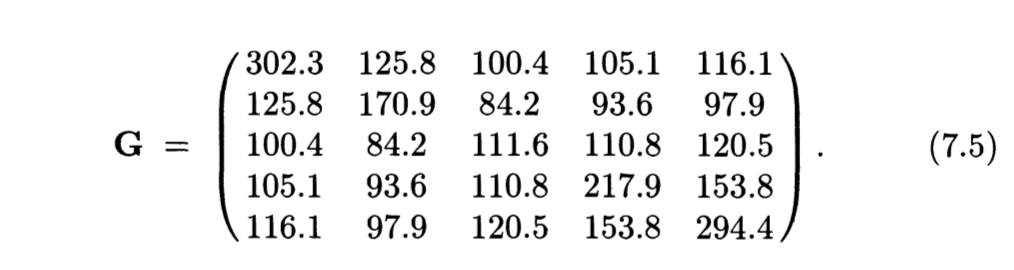
\includegraphics[width=0.85\linewidth]{6/e75.png}
\newline

\setcounter{equation}{5}
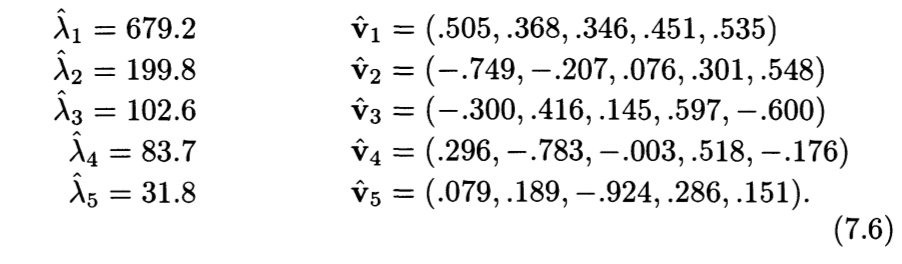
\includegraphics[width=0.85\linewidth]{6/e76.png}
\newline

\setcounter{equation}{6}
Какой интерес представляют собственные значения и векторы ковариационной матрицы? Они помогают описать структуру высокоразмерных данных (как в случае с таблицей (7.1)) в которых описано большое число независимых величин ($n = 88$ студентов), но при этом имеются коррелированные измерения для каждого студента. Заметьте, что пять тестовых оценок высоко коррелированы. Студент, который хорошо сдал тест по механике, вероятно также хорошо сдал тест и по векторам и т.д. Очень простая модель для коррелированных оценок имеет вид
\begin{equation}
	\mathbf x_i = Q_i \mathbf v, \qquad i = 1,2,\ldots,88.
\end{equation}

\noindent
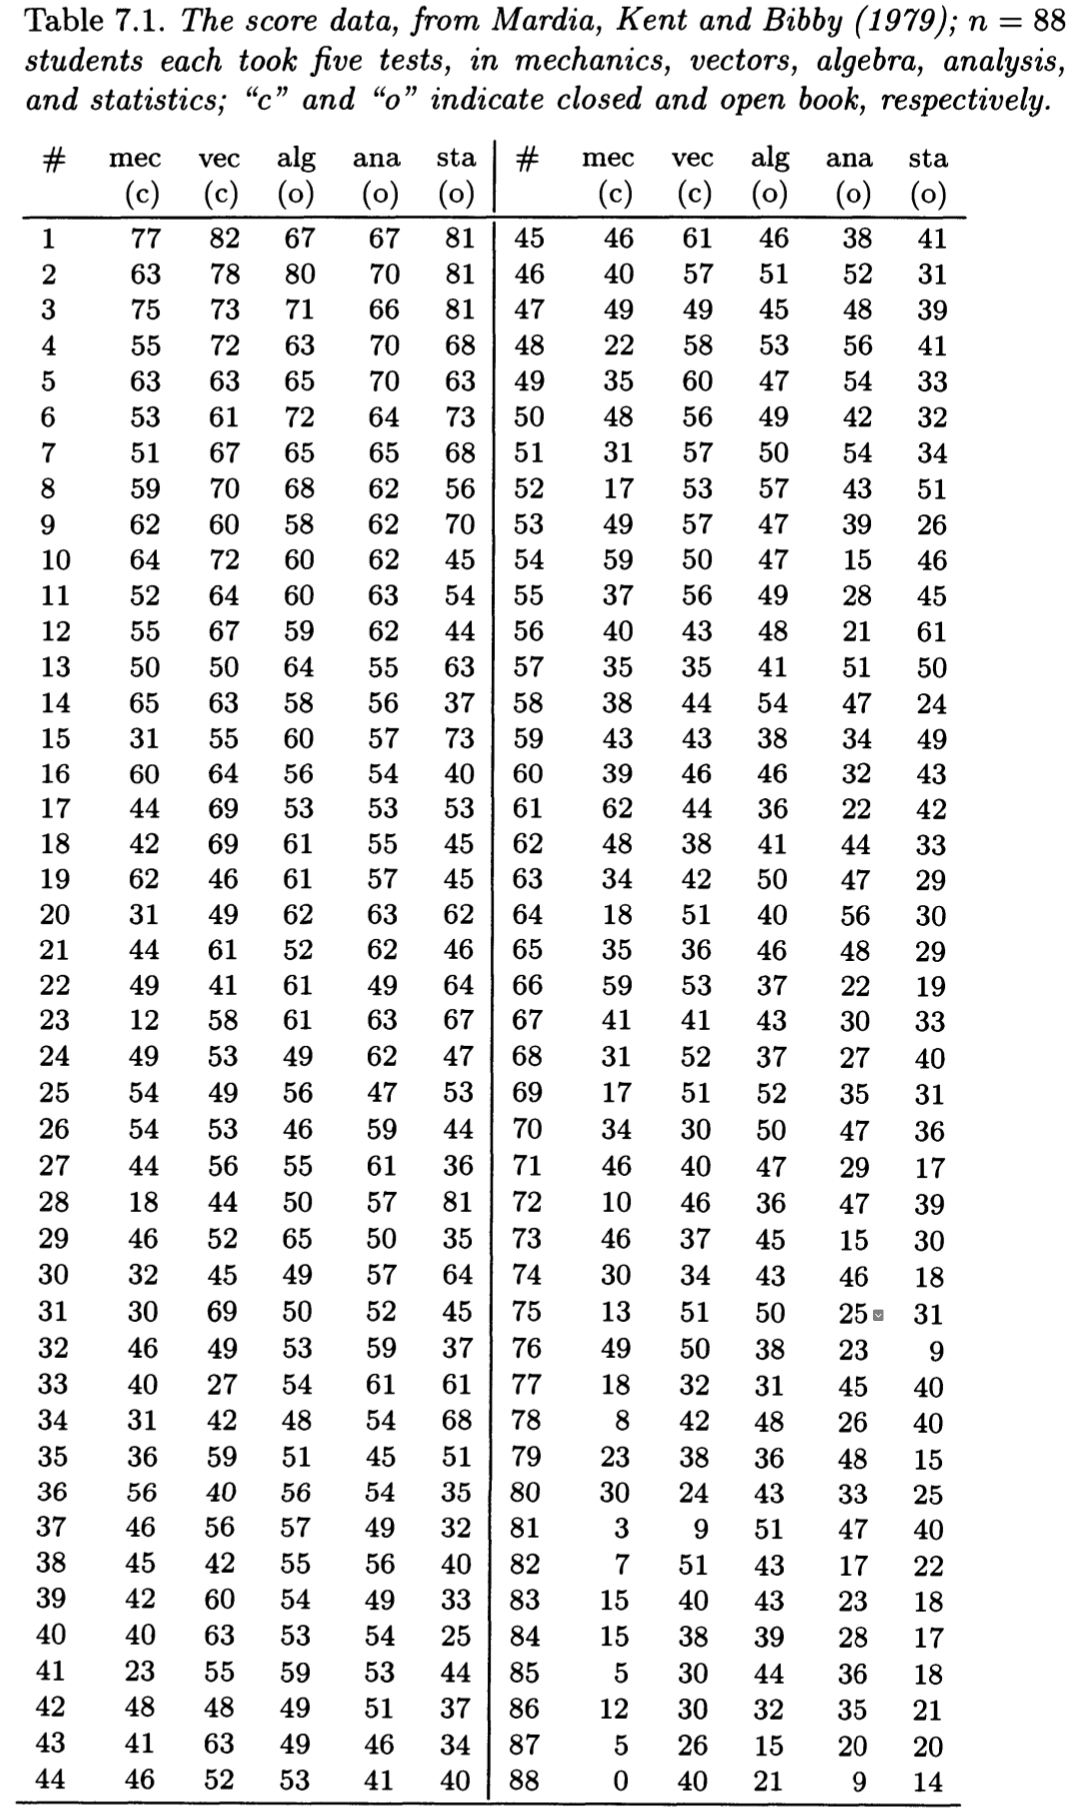
\includegraphics[width=0.9\linewidth]{6/t71.png}
\newline
\setcounter{table}{1}

$Q_i$ является числом, представляющим способности $i$-го студента, в то время как $\mathbf v = (v_1,v_2,v_3,v_4,v_5)$ есть фиксированный вектор из 5 чисел, определённый для всех студентов. $Q_i$ можно рассматривать как общую оценку интеллектуальных способностей студента $i$ (IQ). Изначально IQ были мотивированы именно моделями чуть сложнее, чем (7.7).

Если бы модель (7.7) была верна, мы бы смогли это определить из собственных значений: только $\hat \lambda_1$ было бы положительным, остальные --- $\hat \lambda_2, \hat \lambda_3, \hat \lambda_4, \hat \lambda_5$ --- равнялись бы нулю; также первый собственный вектор $\hat{\mathbf v}_1$ был бы равен $\mathbf v$. Пусть $\hat \theta$ есть частное наибольшего собственного значения и их суммы, то есть
\begin{equation}
	\hat \theta = \hat \lambda_1 / \sum_{i = 1}^5 \hat \lambda_i.
\end{equation}
Модель (7.7) эквивалентна $\hat \theta = 1$. Конечно, мы не можем ожидать, что для таких зашумлённых данных, как оценки, модель (7.7) окажется точной, даже если модель фундаментально верна.

Рисунок 7.1 даёт стилизованную иллюстрацию этого замечания. Мы взяли только две из оценок и отобразили слева ситуацию, если бы одно число $Q_i$ идеально отражало обе оценки. Оценки лежат на одной прямой; $Q_i$ можно считать как расстояние вдоль прямой до каждой точки от начала координат. Рисунок справа показывает более реалистичную ситуацию. Точки не лежат вдоль прямой, но расположены близко к ней. Прямая на графике коллинеарна направлению, заданному первым собственным вектором ковариационной матрицы. Эта прямая иногда называется \textit{прямой первой главной компоненты} и имеет следующее свойство: она минимизирует сумму квадратов расстояний между точками и прямой (в отличие от метода наименьших квадратов, который заключается в минимизации суммы квадратов вертикальных расстояний до прямой). Эти расстояния показаны на рисунке справа в виде небольших отрезков. Сложно создать такой график для всех данных об оценках: прямая главной компоненты была бы прямой в пятимерном пространстве, лежащей ближе всего к данным. Если рассмотреть проекцию каждой из точек на прямую, прямая первой главной компоненты  также будет минимизировать выборочную дисперсию всех спроецированных точек.

Для данных о тестировании студентов получим
\begin{equation}
  \hat \theta = \frac{679.2}{679.2+199.8+\ldots+31.8} = 0.619.
\end{equation}
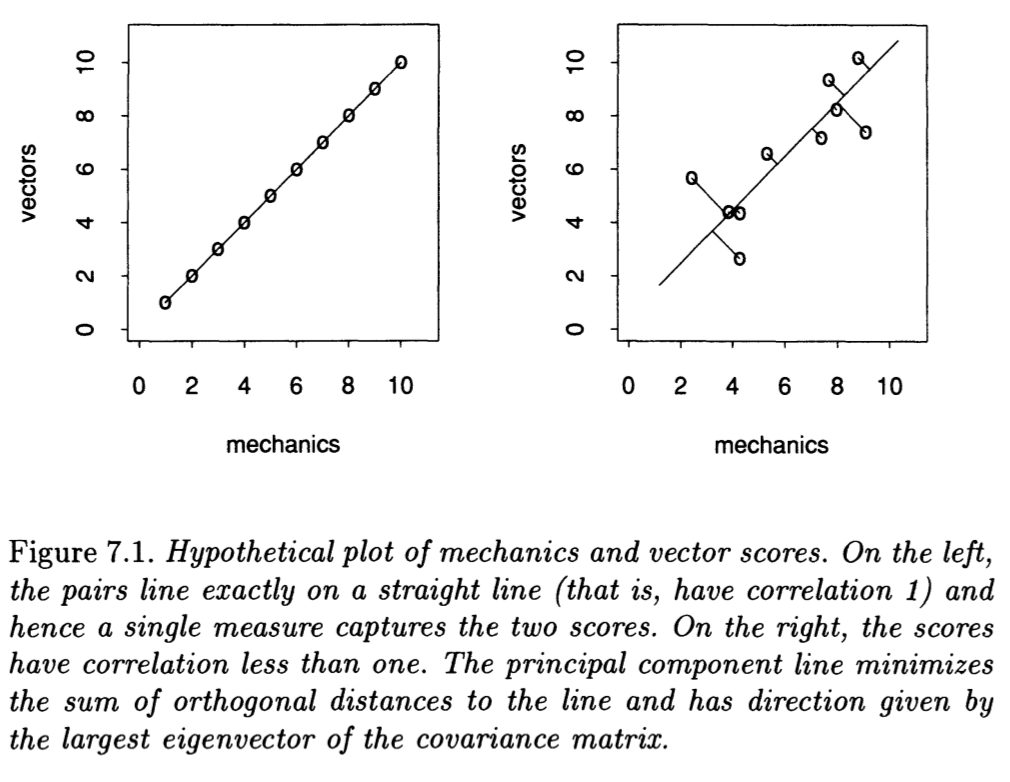
\includegraphics[width=0.85\linewidth]{6/f71.png}
\setcounter{figure}{1}

Во многих ситуациях такое большое значение $\hat \theta$ можно считать достаточно любопытным, что показывает высокую степень предсказательной силы модели (7.7).
Значение $\hat \theta$ измеряет процент дисперсии, объясняемой первой главной компонентой. Чем ближе точки лежат к прямой первой главной компоненты, тем выше значение $\hat \theta$.
Насколько точна оценка $\hat \theta$? Именно для ответа на такие вопросы бутстреп и был создан. Математическая сложность вычисления $\hat \theta$ не важна до тех пор пока мы можем подсчитать $\hat \theta^*$ для любых бутстреп данных. В этом случае бутстреп выборка представлена $\mathbf X^*$ --- матрицей $88\times 5$. Строки $\mathbf x_i^*$ матрицы $\mathbf X^*$ есть случайная выборка размера 88 из столбцов оригинальной матрицы $\mathbf X$
\begin{equation}
	\mathbf x_1^* = \mathbf x_{i_1}^*,\,\mathbf x_2^* = \mathbf x_{i_2}^*, \ldots,\, \mathbf x_{88}^* = \mathbf x_{i_{88}}^*, 
\end{equation}
как в (6.4). Некоторые строки матрицы $\mathbf X$ не появляются ни разу, некоторые один раз, некоторые дважды, и т.д., в итоге имеется 88 строк.

Сгенерировав матрицу $\mathbf X^*$, мы считаем её ковариационную матрицу $\mathbf G^*$ по аналогии с (7.4)
\begin{equation}
G_{jk}^* = \frac{1}{88}\sum_{i = 1}^{88} (x_{ij}^* - \bar x_j^*) (x_{ik}^* - \bar x_k^*), \qquad j,k = 1,2,3,4,5.
\end{equation}

Затем вычисляем собственные значения матрицы $\mathbf G^*$ --- $\hat \lambda_1^*, \hat \lambda_2^*,\ldots,\hat \lambda_5^* $ --- и в конце
\begin{equation}
	\hat \theta^* = \hat \lambda_1^* / \sum_{i = 1}^5 \hat \lambda_i^*,
\end{equation}
На рисунке 7.2 изображена гистограмма $B = 200$ репликаций бутстреп оценок $\hat \theta^*$. 
\newline
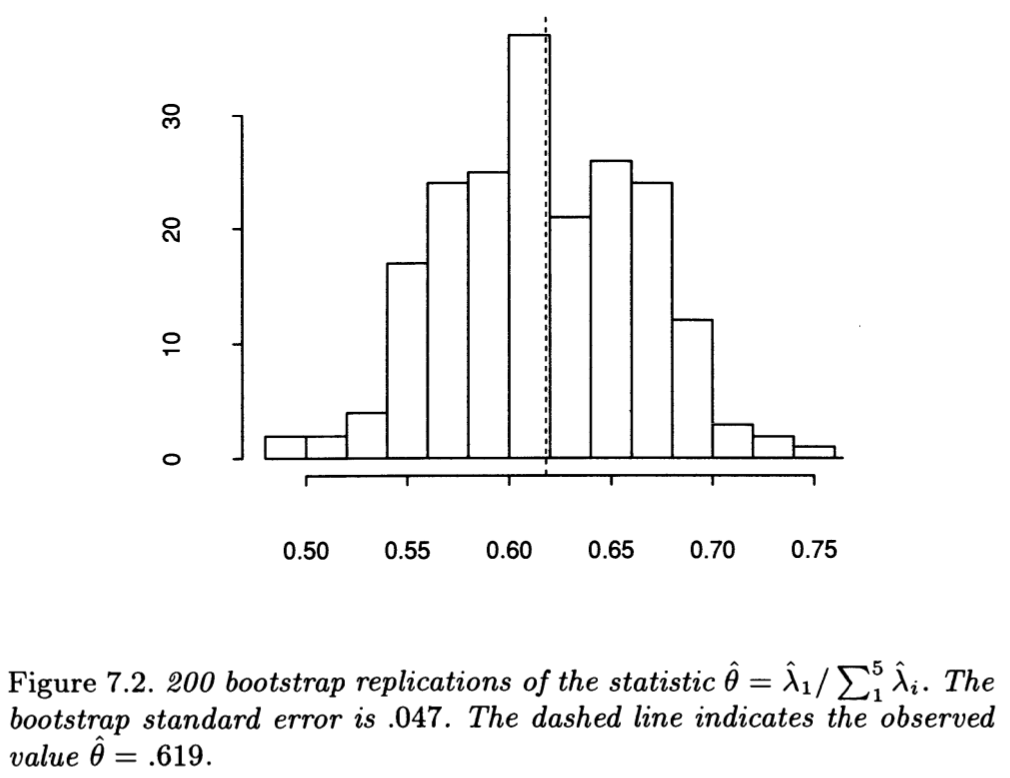
\includegraphics[width=0.85\linewidth]{6/f72.png}
\newline
\setcounter{figure}{2}

Они дают следующую оценку стандартной ошибки $\hat \theta^*$: $\widehat{\text{se}} = 0.047$. Среднее для всех 200 репликаций составило $0.625$, что лишь немногим больше, чем $\hat \theta = 0.619.$ Это означает, что $\hat \theta$ близка к несмещённой. Гистограмма выглядит адекватно, но $B = 200$ всё же недостаточно для того, чтобы ясно увидеть форму распределения. Некоторые квантили эмпирического распределения $\hat \theta^*$ показаны в таблице 7.2.

\noindent
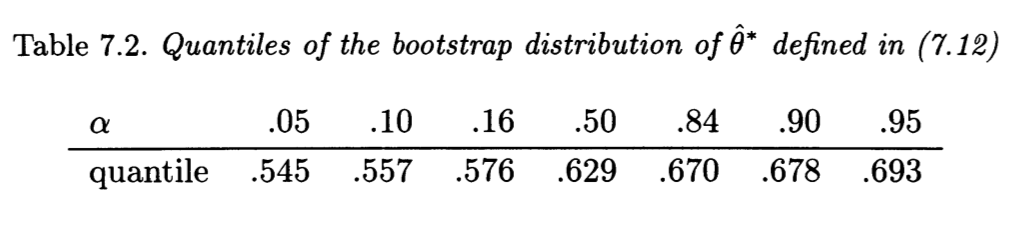
\includegraphics[width=0.9\linewidth]{6/t72.png}
\newline
\setcounter{table}{2}

\textit{Стандартный доверительный интервал} для настоящего значения $\theta$ (значениe $\hat \theta$, если устремить $n \rightarrow \infty$)
\begin{equation}
  \theta \in \hat \theta \pm z^{(1-\alpha)} \cdot \widehat{\text{se}} \qquad \text{(с вероятностью $1 - 2\alpha$)}
\end{equation}
где $z^{(1-\alpha)}$ есть $100(1- \alpha)$ персентиль стандартного нормального распределения; $z^{(.975)} = 1.960,z^{(.95)} = 1.645,z^{(.841)} = 1.000$, и т.д. Вычисление интервала основано на применении асимптотической теории, которая распространяет (5.6) на генеральные статистики $\hat \theta$. В нашем случае 
$$
\theta \in 0.619 \pm 0.047 = [ 0.572,0.666]\quad \text{с вероятностью }  0.683 
$$

$$
\theta \in 0.619 \pm 0.077 = [ 0.542,0.696]\quad \text{с вероятностью }  0.900. 
$$

В 12--14 главах обсуждаются улучшенные бутстреп доверительные интервалы, менее зависимые от асимптотической теории нормального распределения.

Случайный вектор $\hat{\mathbf v}_1$, относящийся к первому собственному значению, называется первой главной компонентой $\mathbf G$. Предположим, что мы хотим выразить результаты студента одним числом, а не пятью (например, для некоторого общего оценивания). Можно показать, что наилучшая линейная комбинация оценок есть 
\begin{equation}
  y_i = \sum_{k=1}^5 \hat{v}_{1k} x_{ik},
\end{equation}
то есть линейная комбинация, использующая компоненты $\hbv_1$ как веса. Эта линейная комбинация --- <<наилучшая>> в смысле того, что среди всех возможных $\mathbf v$ она отражает наибольшую вариативность в данных по пяти оценкам. Если же мы хотим описать успеваемость студента двумя числями, например $(y_i,z_i)$, вторая линейная комбинация должна выглядеть так

\begin{equation}
  y_i = \sum_{k=1}^5 \hat{v}_{2k} x_{ik},
\end{equation}
где веса взяты из второй главной компоненты $\hbv_2$, второго собственного значения матрицы $\mathbf G$.

Веса, заданные главными компонентами, часто дают понимание структуры многомерного набора данных. Для данных с оценками интерпретация будет следующей: первая главная компонента $$\hbv_1 = (0.51, 0.37, 0.35, 0.45, 0.54)$$ накладывает положительные веса примерно одинакового размера на каждый из тестов, то есть $y_i$ условно эквивалентно взятию суммарной (или средней) оценки $i$-го студента. Вторая главная компонента $$\hbv_2 = (-0.75, -0.2, 0.08, 0.30, 0.55)$$ даёт отрицательные веса двум тестам без использования конспекта и положительные на три теста с использованием конспекта, так что $z_i$ есть показатель \textit{разницы} оценок между тестами с открытым и закрытым конспектом для $i$-го студента. (Студент с высокой оценкой $z$ гораздо лучше справился с тестами с открытым конспектом, чем с закрытым.)

Векторы главных компонент $\hbv_1$ и $\hbv_2$ есть суммарные статистики, как и $\thetahat$, несмотря на то, что у каждой из них есть несколько компонент. Мы можем применить бутстреп анализ для того, чтобы узнать, насколько они устойчивы. Те же 200 бутстреп выборок, с помощью которых мы получили $\thetahat^*$, дают бутстреп репликации $\hbv_1^*$ и $\hbv_2^*$. Они могут быть посчитаны как первые два собственных вектора $\mathbf G^*$, (7.11).

В таблице 7.3 показаны $\seh_{200}$ для каждой из компонент векторов $\hbv_1$ и $\hbv_2$. Первое, что можно заметить --- это более высокую точность $\hbv_1$; бутстреп стандартная ошибка компонент $\hbv_1$ составляет менее половины ошибки $\hbv_2$. В таблице 7.3 также указаны основанные на персентилях робастные бутстреп стандартные ошибки $\sew_{200,\alpha}$, посчитанные для $\alpha = 0.84, 0.9, 0.95$. Для компонент $\hbv_1$ $\sew_{200, \alpha}$ примерно равно $\seh_{200}$. 
\\~\\
\noindent
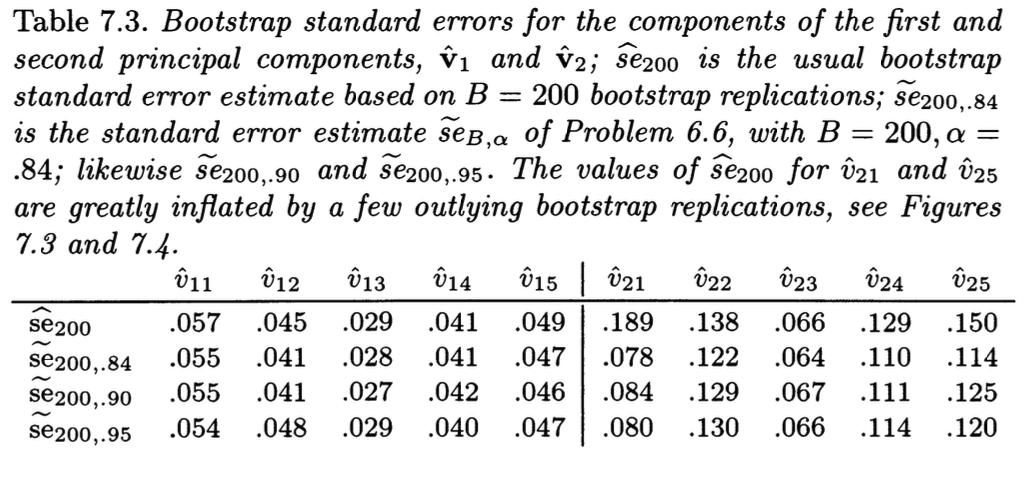
\includegraphics[width=0.9\linewidth]{6/t73.png}
\newline
\setcounter{table}{3}
Это не так для $\hbv_2$, в особенности для первой и пятой координаты. На рисунке 7.3 можно увидеть, в чём проблема. На рисунке показаны эмпирические распределения для 200 бутстреп репликаций $\hat v_{ik}^*$, в отдельности для каждого из $i = 1,2,\, k = 1,2,\ldots, 5$. Эмпирические распределения отражены ящиками с усами. Отрезок в центре ящика --- медиана распределения; нижняя и верхняя сторона ящика есть есть соответственно 25-я и 75-я персентиль распределения; усы покрывают всё распределение за исключением некоторых выбросов (определённых по некоторому критерию), которые отмечены звёздочкой.
\\~\\
\noindent
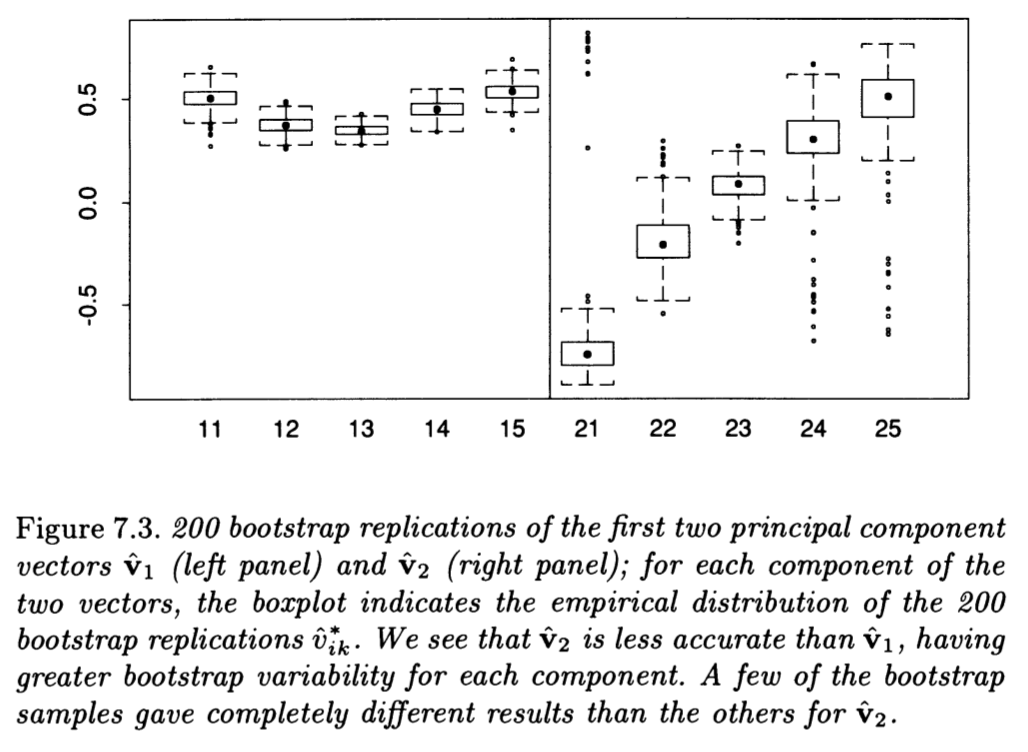
\includegraphics[width=0.9\linewidth]{6/f73.png}
\newline
\setcounter{figure}{3}

Можно увидеть, что большие значения $\seh_{200}$ для $\hat v_{21}$ и $\hat v_{25}$ вызваны несколькими выделяющимися значениями $\hat v_{ik}^*$. Приближённый доверительный интервал $\theta \in \thetahat \pm z^{1-\alpha} \seh$ будет более точным, если выбрать $\sew_{200, \alpha}$ в качестве оценки $\seh$, как минимум для умеренных значений $\alpha$ таких, как $0.843$. Гистограмма значений  $v^*_{21}$ имеет форму нормального распределения со средним в точке $-0.74$ и стандартным отклонением $0.075,$ с небольшим числом точек далеко от гистограммы. Это показатель того, что с малой вероятностью, порядка $1\%$ или $2\%$, что $\hat v_{21}$ оказывается совершенно неточной оценкой настоящего значения $v_{21}$. Если же данное событие не произошло, $\hat v_{21}$ вероятно находится в пределе одного или двух $\sew_{200}$ от $v_{21}$.

На рисунке 7.4 показаны графики бутстреп репликаций $$
\hbv_1^*(b)\tx{ и } \hbv_2^*(b),\qquad b=1,2,\ldots, 200,
$$ 
соединяющие компоненты каждого вектора прямыми. Это более наглядный (хоть и менее точный) показатель вариативности $\hbv_2$, чем предложенные ранее в таблице 7.3 и на рисунке 7.3.
Три конкретных репликации, отмеченные числами 1, 2, и 3, являются выбросами на нескольких компонентах.
\\~\\
\noindent
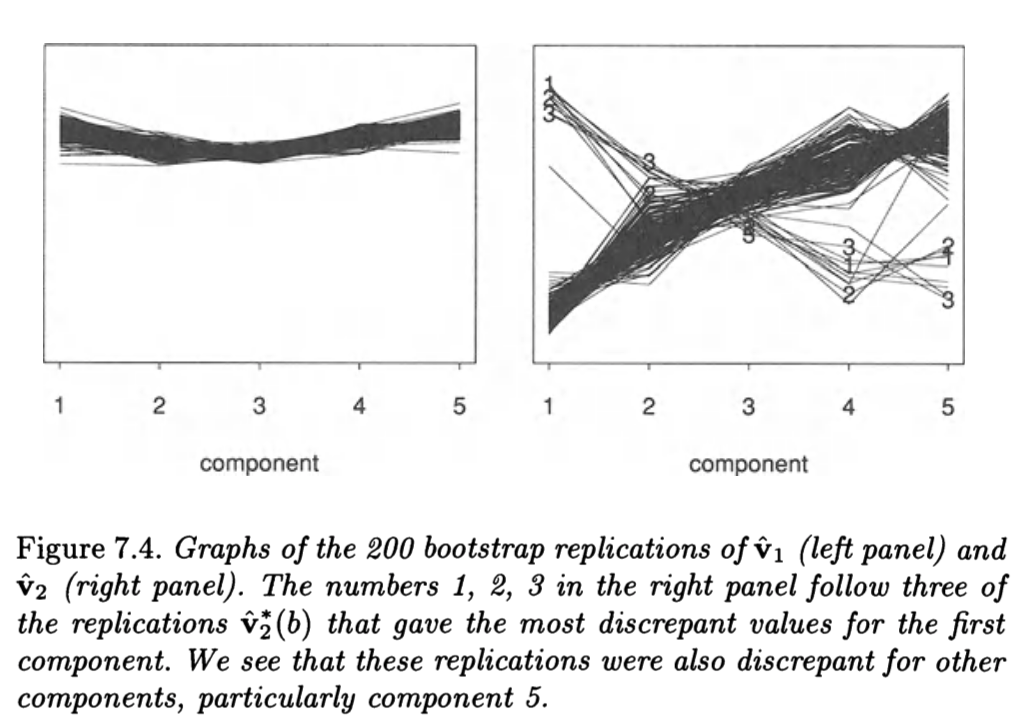
\includegraphics[width=0.9\linewidth]{6/f74.png}
\newline
\setcounter{figure}{4}

Читатель, которому знаком метод главных компонент, может теперь увидеть, что сложности со вторым собственным вектором объясняются проблемой единственности собственных векторов.
Технически, определение собственного вектора $\mathbf v$ также верно и для обратного ему вектора $- \mathbf v$. Алгоритм, который считает собственные числа и собственные значения, может приводить решения с разными знаками у $\hbv_1,\hbv_2,\ldots$ Репликации 1 и 2 привели к матрицам $\X^*$, для которых знак $\hbv_2^*$ получился обратным. Такая неопределённость обычно не важна при определении статистических особенностей оценок (хотя хорошо замечать такую неопределённость на основании результата применения бутстрепа). Если перестать учитывать 1 и 2, как происходит при оценке $\sew_{200,\alpha}$, мы видим, что $\hbv_2$ всё равно менее точна, чем $\hbv_1$.






\section{Пример 2: построение кривой по данным}

В этом примере мы будем оценивать функцию регрессии двумя способами, сначала с помощью стандартного метода наименьших квадратов, а затем с помощью современного метода построения кривой по данным, который называется \textit{loess}. Мы начнём с краткого повторения теории регрессии. В главе 9 снова рассматривается задача регрессии и дан альтернативный бутстреп метод для оценки стандартных ошибок регрессии. На рисунке 7.5 показан типичный набор данных, для которого используются регрессионные методы:  мужчин приняли участие в эксперименте, чтобы определить, уменьшает ли лекарство на основе холостирамина уровень холестерина в крови. Мужчины должны были принимать по 6 пакетиков холостирамина в день, однако многие из них принимали гораздо меньше.
\\~\\
\noindent
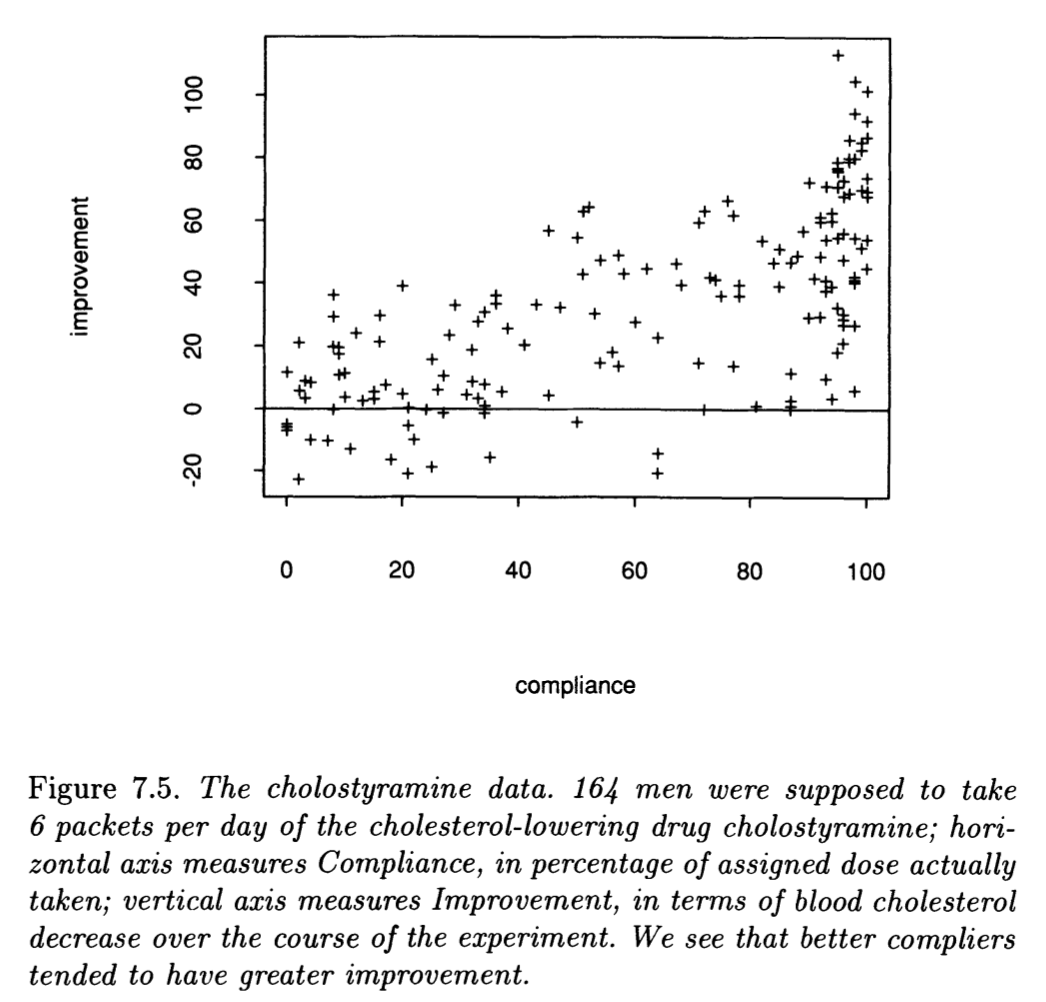
\includegraphics[width=0.9\linewidth]{6/f75.png}
\newline
\setcounter{figure}{1}

Горизонтальная ось, которую мы назовём <<$z$>>, измеряет <<Соответствие>>, то есть процент приёма от назначенной дозы,
$$
z_i = \text{ процент соответствия для мужчины } i,\, i = 1,2,\ldots, 164.
$$

Соответствие измерялось подсчётом количества пакетиков, которые вернули индивиды. Те, кто приняли все пакетики, находятся в правом краю графика; те, кто не принимал ничего --- в левом. Горизонтальная ось, отмеченная <<$y$>>, есть показатель \textit{Улучшения}, уменьшение уровня холестерина в кровяной плазме за время исследования,
$$
y_i = \text{ уменьшение уроня холестерина в крови для индивида } i,\, i = 1,2,\ldots, 164.
$$
Полный набор данных представлен в таблице 7.4.
\\~\\
\noindent
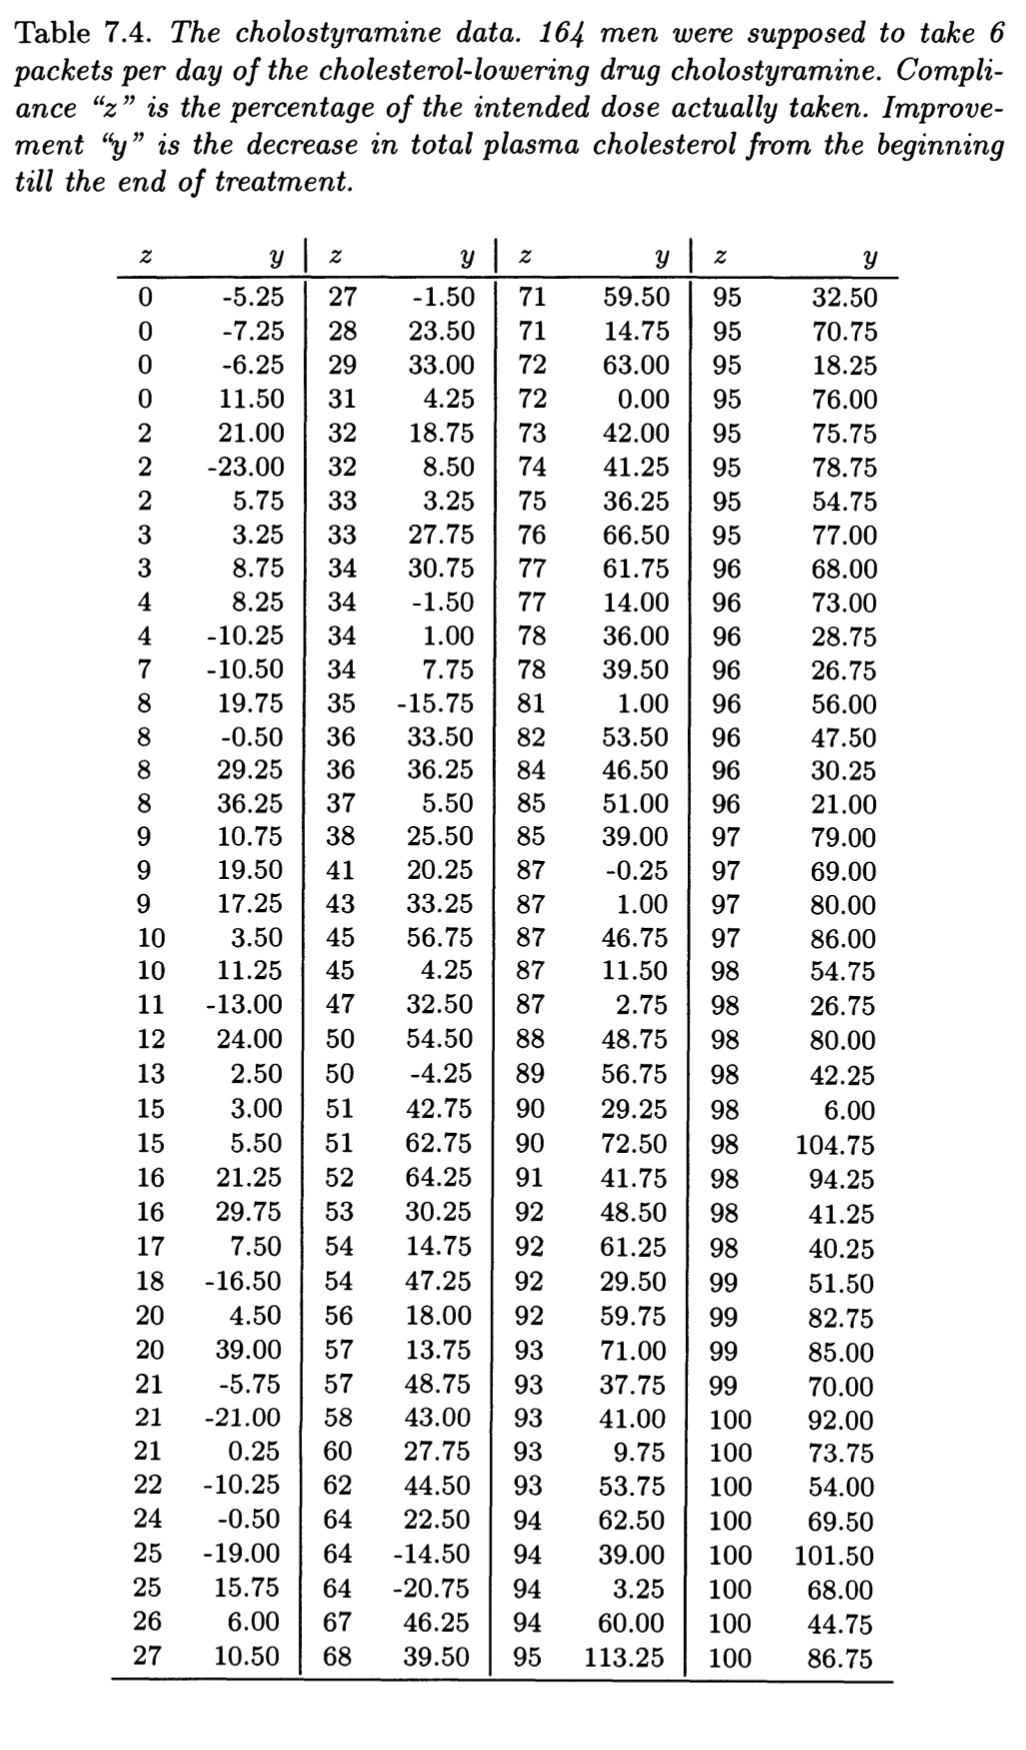
\includegraphics[width=0.95\linewidth]{6/t74.png}
\newline
\setcounter{table}{4}

 На рисунке видно, что мужчины, которые принимали больше хлоростирамина, в целом улучшили свои показатели холестерина, что и ожидалось. То, что мы видим на рисунке 7.5, или скорее то, что мы хотели бы видеть, есть увеличение среднего ответа $y$ в то время как $z$ увеличивается от 0 до $100\%$. На рисунке 7.6 показаны данные вместе с двумя графиками,
\begin{equation}
\hat r_\text{quad}(z) \text{ и }  \hat r_\text{loess}(z).
\end{equation}
\\~\\
\noindent
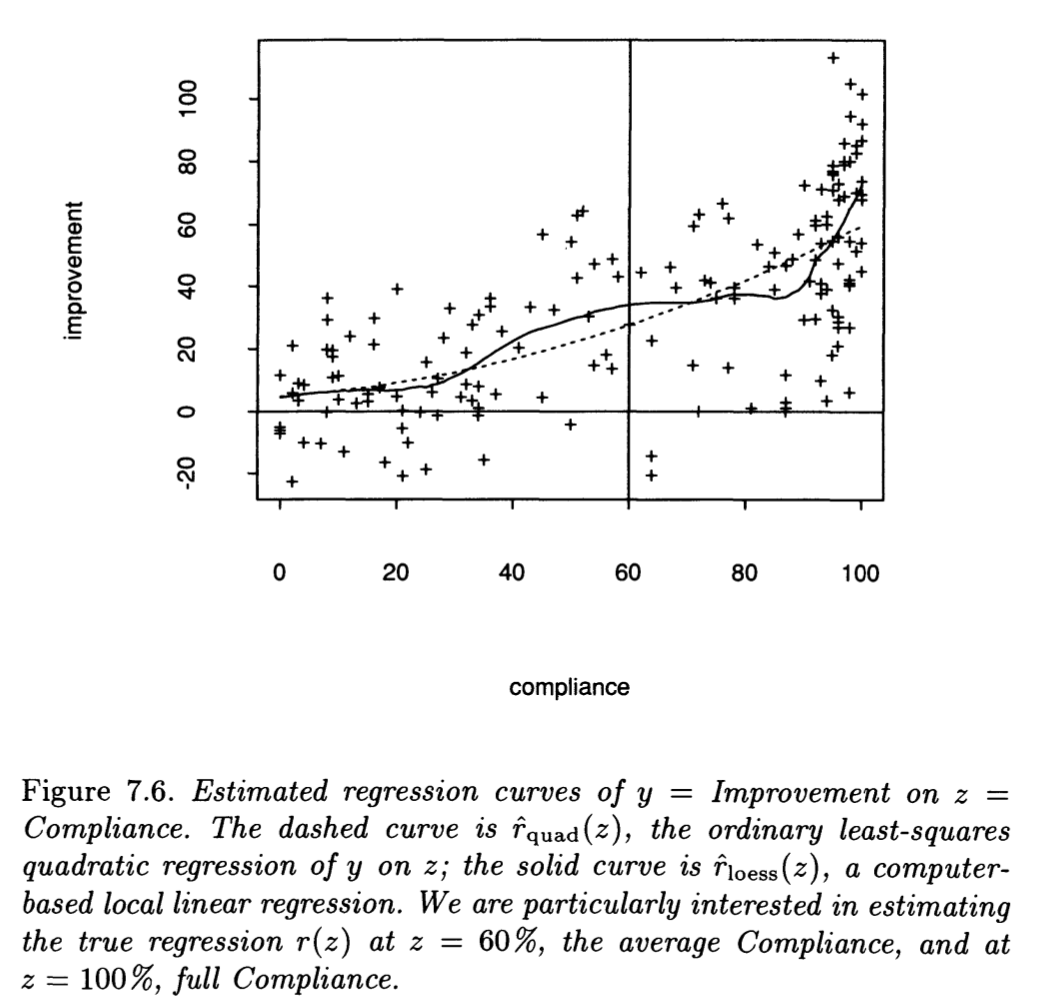
\includegraphics[width=0.9\linewidth]{6/f76.png}
\newline
\setcounter{figure}{7}

Каждый из них есть оценка кривой регрессии. Сейчас будет краткое повторение построения и оценки регрессионных кривых.
По определению регрессией ответа $y$ на независимую переменную $z$ называется условное математическое ожидание $y$ при некотором $z$,
\begin{equation}
  r(z) = \mathrm E(y|z).
\end{equation}
Предположим, что нам была доступна вся популяция $\mathcal U$ мужчин, подходящих для эксперимента, и мы получили набор $\mathcal X = (X_1,X_2,\ldots, X_N)$ оценок \textit{Соответствие-улучшение} $X_j = (Z_j, Y_j),\, j = 1,2,\ldots,N.$ Далее для каждого значения $z$, например $z = 0\%,1\%,2\%,\ldots,100\%$, регрессия была бы условным математическим ожиданием (7.17),
\begin{equation}
  r(z) = \frac{\text{сумма значений $Y_j$ для мужчин в $\mathcal X$ с $Z_j = z$}}{\text{число мужчин в $\mathcal X$ с $Z_j = z$}}.
\end{equation}
 Другими словами, $r(z)$ есть математическое ожидание $Y$ для субпопуляции мужчин, у которых $Z= z$.
 
 Разумеется у нас нет целой популяции $\mathcal X$. У нас имеется выборка $\mathbf x = (\mathbf x_1, \mathbf x_2, \ldots, \mathbf x_{164})$, где $\mathbf x_i = (z_i, y_i)$, как показано на рисунке 7.5 и в таблице 7.4. Как мы можем оценить $r(z)$? Очевидная оценка методом подстановки есть
 \begin{equation}
  \hat r(z) = \frac{\text{сумма значений $y_j$ для мужчин в $\mathbf x$ с $z_j = z$}}{\text{число мужчин в $\mathbf x$ с $z_j = z$}}.
\end{equation}

Можно представить себе разбиение на вертикальные полосы шириной в $1\%$ на рисунке 7.5 и усреднение значений на каждой полосе для получения $\hat r(z).$ Результаты можно увидеть на рисунке 7.7.
\\~\\
\noindent
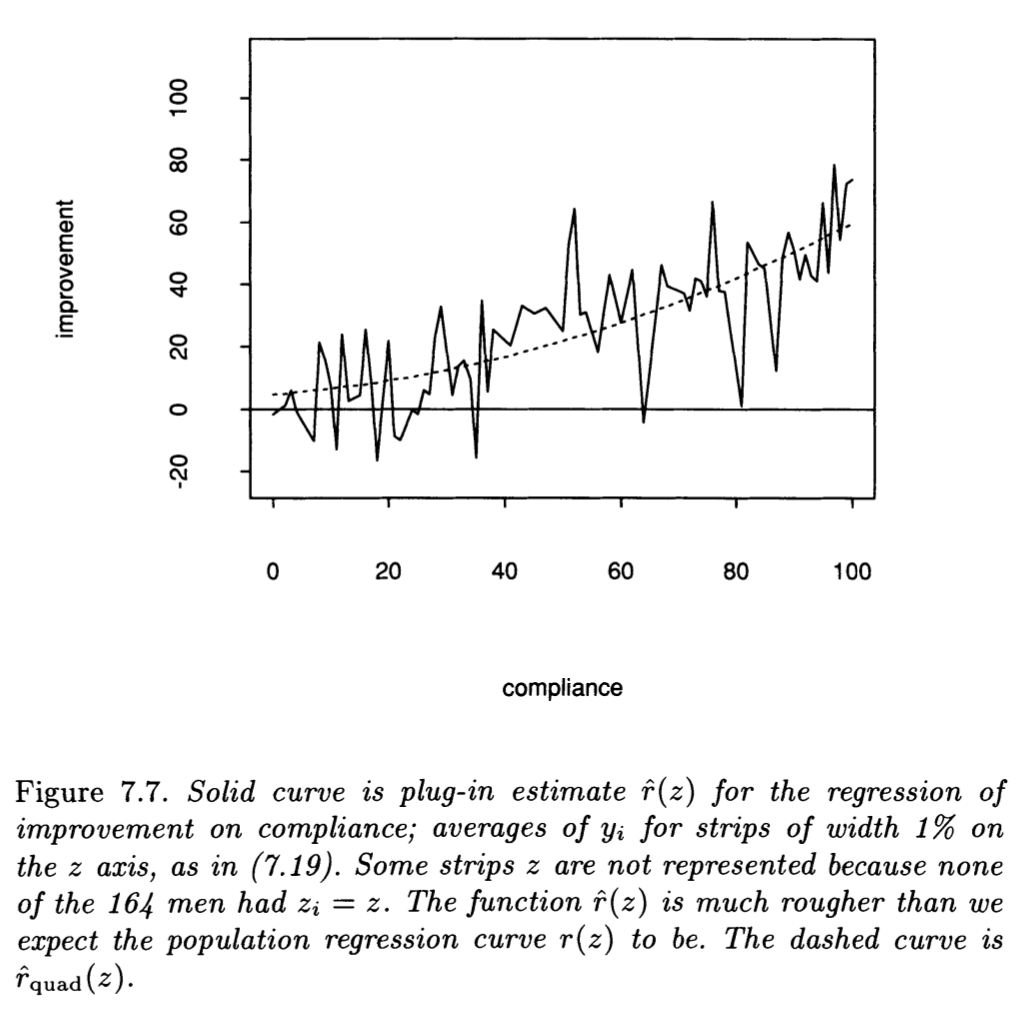
\includegraphics[width=0.9\linewidth]{6/f77.png}
\newline
\setcounter{figure}{7}

Впервые нашёлся пример, для которого метод подстановки работает не очень хорошо. Оценка регрессии $\hat r(z)$ гораздо грубее, чем мы хотели бы для оценки популяционной регрессии $r(z)$. Проблема в том, что внутри каждой полосы шириной в $1\%$ точек для адекватной оценки $r(z)$ недостаточно. Для некоторых полос шириной в $5\%$ точек внутри нет вообще. Мы можем увеличить ширину промежутка, скажем, до $10\%$ вместо $1\%$, но это не исправит проблему небольшого числа точек и, вероятно, проблема неустойчивости всё равно останется. На самом деле, имеется более элегантное и эффективное решение, которое основано на методе наименьших квадратов.

Использование метода начинается с предположения, что популяционная регрессионная функция, какая бы она не была, принадлежит семейству $\mathcal R$ гладких функций, индексированных вектором параметров $$\bm \beta = (\beta_0,\beta_1,\ldots,\beta_p)^\mathrm{T}$$. Для рассматриваемого примера мы ограничимся семейством квадратичных функций от $z$, скажем, $\mathcal R_\text{quad},$
\begin{equation}
  \mathcal R_\text{quad: \quad} r_{\bm \beta}(z) = \beta_0 + \beta_1 z + \beta_2 z^2,
\end{equation}
поэтому $\bm \beta = (\beta_0,\beta_1,\beta_2)^\mathrm{T}$. Далее мы обсудим выбор именно квадратичного семейства $\mathcal R_\text{quad},$ но на сейчас примем это как данное.

Читатель может представить себе выбор некоторого пробного значения $\bm \beta$, к примеру, $\bm \beta = (0,0.75,0.005)^\mathrm{T}$, и построение $r_\beta(z)$ на рисунке 7.5. Мы хотели бы, чтобы кривая $r_\beta(z)$ проходила близко к нашим данным $(z_i, y_i)$ в некотором общем смысле. Наиболее удобно для вычислений измерять близость кривой к данным с помощью суммы квадратов остатков (\textit{Residual Squared Error}),
\begin{equation}
  \rse(\bm \beta) = \sum_{i = 1}^n [y_i - r_{\bm \beta} (z_i)]^2.
\end{equation}
Сумма квадратов остатков получается опусканием вертикальных отрезков от каждой точки $(z_i, y_i)$ к кривой $r_{\bm \beta} (z_i)$, а затем суммированием квадратов их длин.

\textit{Метод наименьших квадратов}, созданные Гауссом и Лежандром в начале 19 века, выбирает среди кривых в $\mathcal R$ те, которые минимизируют $\rse$. Наилучший из них объявляется $r_{\hat {\bm \beta}}(z),$ где $\hat {\bm\beta}$ минимизирует $\rse(\bm \beta)$,
\begin{equation}
  \rse(\hat{\bm \beta}) = \min_{\bm \beta}{\rse(\bm \beta)}.
\end{equation}
 Кривая $\rquad(z)$ на рисунке 7.6 есть $r_{\hat{\bm \beta}}(z) = \hat \beta_0 + \hat \beta_1 z + \hat \beta_2 z^2,$ наилучшая квадратичная функция для наших данных.
 
 Лежандр и Гаусс обнаружили замечательную явную формулу для решения $\hat{\bm \beta}$ задачи наименьших квадратов. Пусть $\mathbf C$ есть матрица $164\times 3,$ $i$-я строка которой есть
 \begin{equation}
  \bm c_i = (1, z_i, z_i^2),
\end{equation}
и пусть $\mathbf y$ есть вектор из 164 значений $y_i.$ Тогда, используя стандартную матричную нотацию, имеем
\begin{equation}
  \hat{\bm \beta} = (\mathbf C^\mathrm{T} \mathbf{C})^{-1} \mathbf{C}^\mathrm{T} \mathbf y.
\end{equation}
Более  подробно мы рассмотрим эту формулу в главе 9. Для наших целей, связанных с применением бутстрепа, нам достаточно лишь знать про то, что набор данных из $n$ пар $\mathbf x = (\mathbf x_1, \mathbf x_2,\ldots, \mathbf x_n)$ приводит к получению квадратичной кривой $r_{\hat{\bm \beta}}(z)$ через отображение $\mathbf x \rightarrow r_{\hat{\bm \beta}}(z),$ которое описывается (7.23), (7.24) и (7.20).

Можно рассматривать $r_{\hat{\bm \beta}}(z)$ как сглаженную версию оценки по методу подстановки $\hat r(z)$. Предположим, что мы бы рассмотрели более широкий класс гладких функций $\mathcal R,$ к примеру, класс кубических функций $\mathcal R_\text{cubic}.$ В таком случае решение по методу наименьших квадратов $r_{{\hat{\bm\beta}}}(z)$ стало бы ближе к данным, однако оказалось бы более <<бугристым>>, чем квадратичное решение по методу наименьших квадратов. Если бы мы начали рассматривать полиномы всё большей степени, $r_{\hat{\bm \beta}}$ всё больше бы походил на оценку по методу подстановки $\hat r  (z)$. Выбор семейства квадратичных функций основан на нашем представлении о том, насколько гладкой должна быть оригинальная функция регрессии $r(z)$.
 Смотря на рисунок 7.7, мы явно видим, что $\rquad(z)$ гораздо более гладкая, чем $\hat r (z),$ однако в целом соответствует $\hat r (z)$ как функция от $z$.
 
Легко поверить, что настоящая функция регрессии $r(z)$ есть гладкая функция от $z$.  Сложнее поверить в то, что $r(z)$ является квадратичной от $z$ для всех значений $z$. Сглаживающая функция \textit{loess} является компромиссом между \textit{глобальными} предположениями о форме и чисто \textit{локальным} усреднением $\hat r(z)$.  

Для использования loess нужно указать число $\alpha$, которое равно части $n$ точек, используемых при построении кривой в каждой из точек. Кривая $\rloess (z)$ на рисунке 7.6 построена при выборе $\alpha = 0.3$. Для каждого из значений $z$ значение $\rloess (z)$ получается следующим образом:
\begin{enumerate}
	\item $n$ точек $\mathbf x_i = (z_i, y_i)$  упорядочиваются согласно $|z_i - z|,$ а ближайшие $\alpha \cdot n$ точек с наименьшим $|z_i - z|$, запоминаются. Назовём эти точки $\mathcal N(z)$.\footnote{при выборе $\alpha= 0.3, n=164$, алгоритм выбирает в $\mathcal N(z)$ 49 точек}
	\item Взвешенная линейная регрессия (с минимизацией наименьших квадратов) 
	\begin{equation}
  	\hat r_z(Z) = \hat \beta_{z,0} + \hat \beta_{z,1} Z
	\end{equation}
	производится для $\alpha \cdot n$ точек в $\mathcal N(z)$. [То есть коэффициенты $ \hat \beta_{z,0}$ и $\hat \beta_{z,1}$ выбираются как минимизирующие $\sum_{\mathbf x_j \in \mathcal N} w_{z,j} [y_j - (\beta_0 + \beta_1 z_j)]^2$, где веса $w_{z,j}$ есть положительные числа, зависящие от $|z_j - z|$. Взяв 
	\begin{equation}
  u_j = \frac{|z_j - z|}{\max_{\mathcal N (z)}|z_k - z|},
\end{equation}
веса $w_j$ выбираются равными $(1 - u_j^3)^3$.]

	\item В итоге, $\rloess (z)$ назначается равным числу $\hat r_z(Z)$ в точке $Z = z,$
\begin{equation}
  \rloess(z) = \hat r_z (Z=z).
\end{equation}
\end{enumerate}
~\\
\noindent
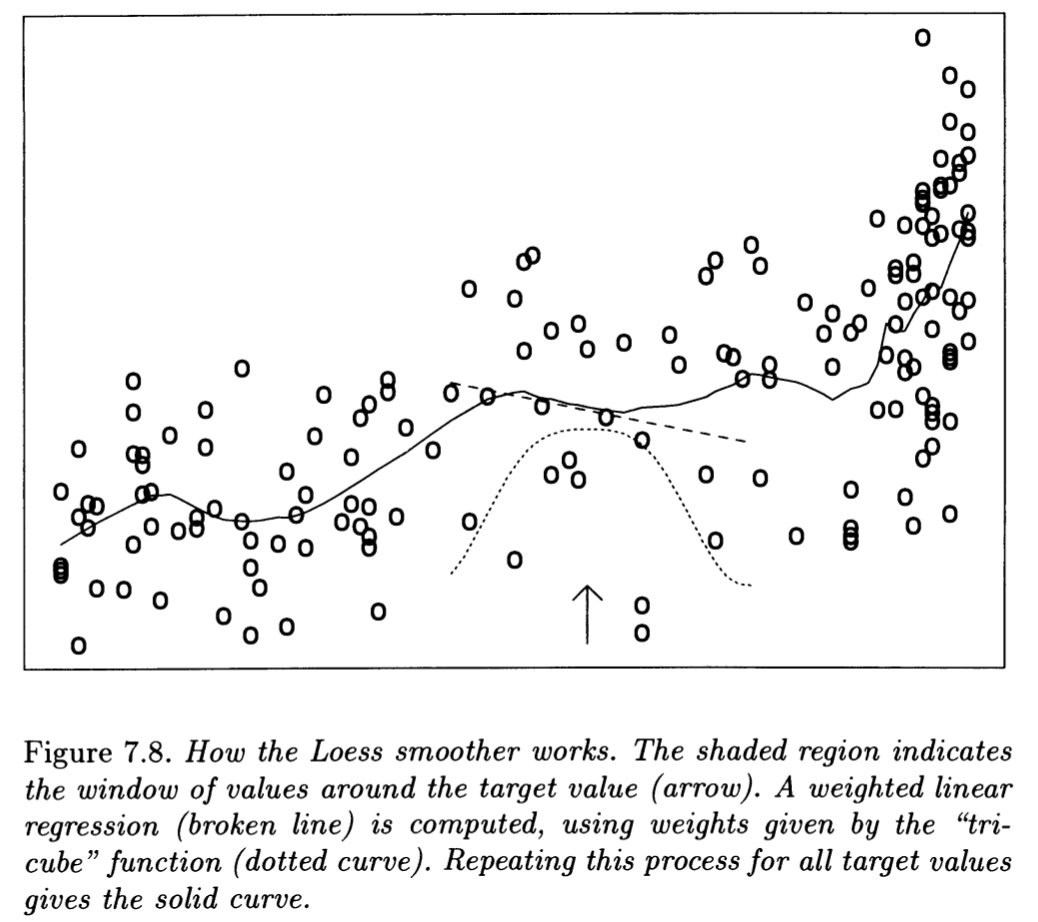
\includegraphics[width=0.9\linewidth]{6/f78.png}
\newline
\setcounter{figure}{8}

Компоненты loess сглаживания показаны на рисунке 7.8. В таблице 7.5 показано сравнение $\rquad(z)$ и $\rloess(z)$ в двух значениях, представляющих наибольший интерес, $z = 60\%$ и $z = 100\%$. Стандартные ошибки по бутстрепу даны для каждого из значений. Они были получены из $B = 50$ бутстреп репликаций алгоритма, показанного на рисунке 6.1.
\\~\\
\noindent
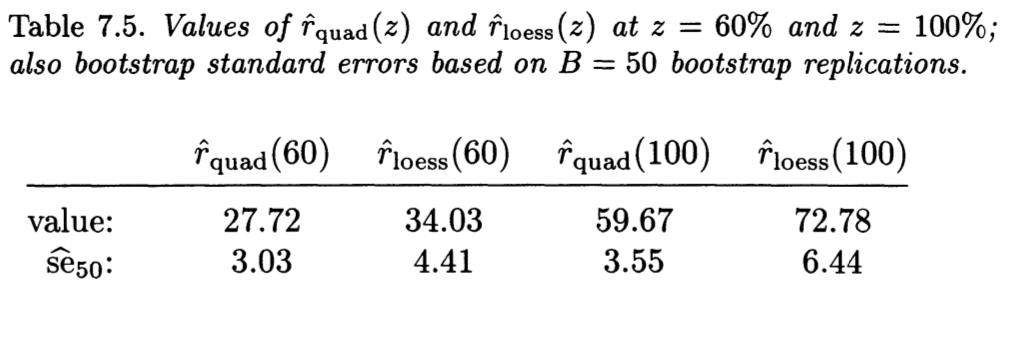
\includegraphics[width=0.9\linewidth]{6/t75.png}
\newline
\setcounter{table}{5}

В данном случае $\hat F$ есть распределение, дающее вероятность $1/164$ каждому из 164 наблюдений $\mathbf x_i = (z_i, y_i).$ Бутстреп набор есть $\mathbf x^* = (\mathbf x_1^*,\mathbf x_2^*, \ldots, \mathbf x_{164}^*),$ где каждый из $\mathbf x_i^* $ равен одному из 164 наблюдений с одинаковой вероятностью. Получив $\mathbf x^*,$ мы вычислили $\rquad^*(z)$ и $\rloess^*(z)$, квадратичную и loess кривые на основе $\mathbf x^*.$ В завершение мы вычислили значения $\rquad^*(60)$ и $\rloess^*(60)$, а также $\rquad^*(100)$ и $\rloess^*(100)$. $B = 50$ значений $\rquad^*(60)$ имеют стандартную ошибку $3.03$ и т.д., см. таблицу 7.5.

Посмотрев на результаты в таблице 7.5, можно сделать вывод о том, что оценка $\rloess(z)$ значительно менее точна, чем $\rquad(z).$	Это неудивительно, ведь $\rloess(z)$ строится на меньшем количестве данных (размер обусловлен $\alpha$), чем $\rquad(z)$. Неустойчивость $\rloess(z)$ очевидна по графикам на рисунке 7.9.
\\~\\
\noindent
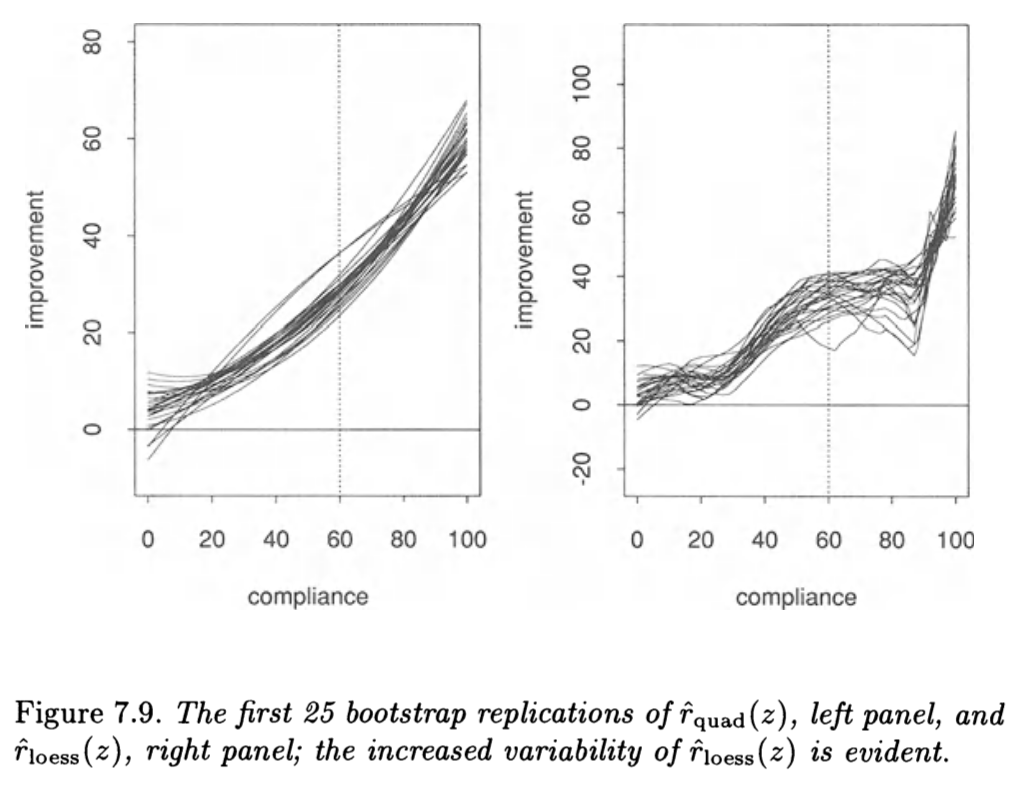
\includegraphics[width=0.9\linewidth]{6/f79.png}
\newline
\setcounter{figure}{9}

Полезно построить кривые бутстрепа, чтобы увидеть, сохраняются ли некоторые интересные особенности оригинальной кривой у кривых по бутстреп выборкам. Например, на рисунке 7.6 видим, что $\rloess(z)$ растёт гораздо быстрее с $z = 80\%$ до $z = 100\%$, чем с $z = 60\%$ до $z = 80\%$. Разность средних у углов наклона составляет
\begin{align}
	\thetahat &= \frac{\rloess(100) - \rloess(80)}{20} - \frac{\rloess(80) - \rloess(60)}{20}\nonumber \\
	&= \frac{672.78 - 37.50}{20} - \frac{32.50 - 34.03}{20} = 1.84.
\end{align}
  
Соответствующее число для $\rquad$ составляет лишь $0.17$. Большинство loess кривых показывают похожий быстрый рост примерно на $80\%$. Ни одно из бутстреп значений $\thetahat^*$ не было меньше нуля, минимум составил 0.23, большинство значений оказались больше единицы, см. рисунок 7.10.
\\~\\
\noindent
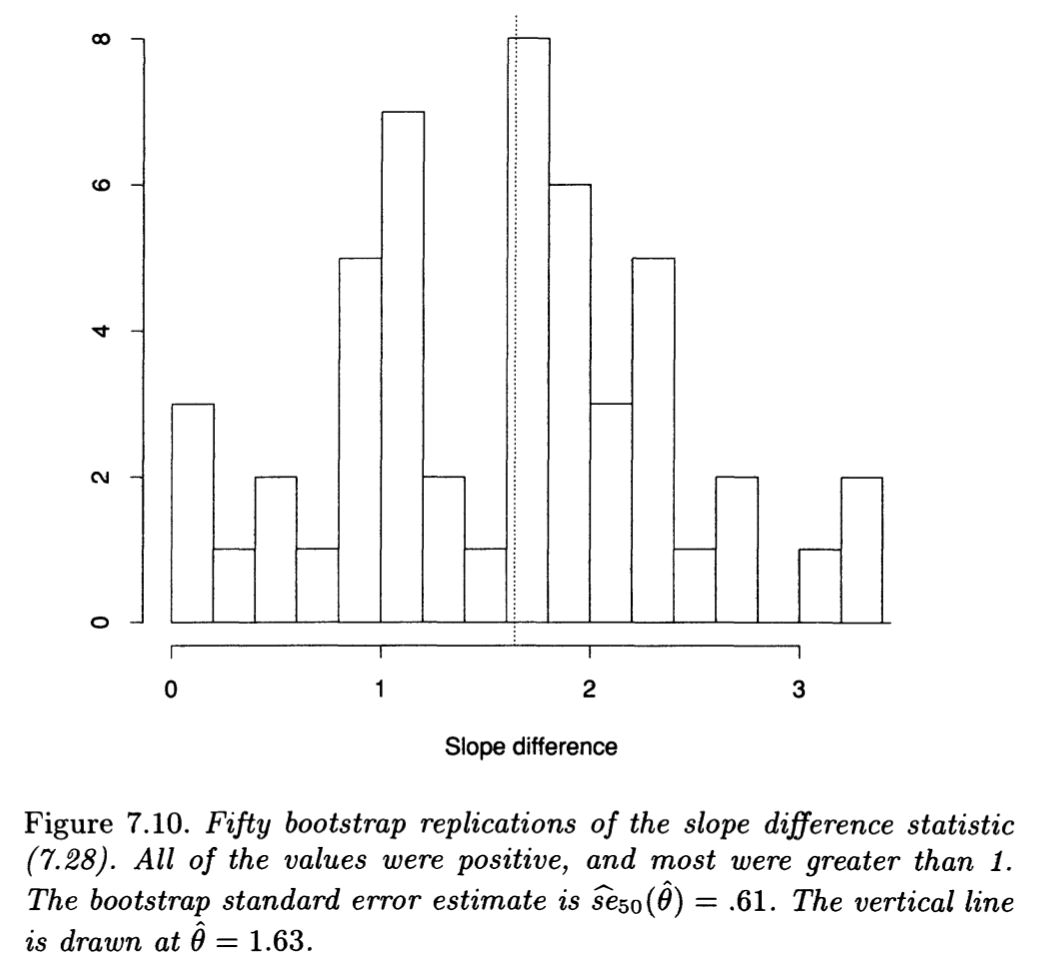
\includegraphics[width=0.9\linewidth]{6/f710.png}
\newline
\setcounter{figure}{10}
В такой момент мы можем законно опасаться того, что $\rquad(z)$ является \textit{слишком} гладкой оценкой оригинальной регрессионной функции $r(z)$. Если значение настоящей разности в углах наклона
\begin{equation}
  \theta = \frac{r(100) - r(80)}{20} - \frac{r(80) - r(60)}{20}
\end{equation}
и находится около $\thetahat = 1.59,$ то $r(z)$ будет выглядеть скорее как 
$\rloess(z)$, чем $\rquad(z)$ для $z$ между 60 и 100. Оценки, построенные на $\rloess(z)$ обычно отличаются высокой дисперсией, как в таблице 7.5, но в то же время имеют низкое смещение. Оба этих свойства происходят от локального характера алгоритма loess, который строит оценку $r(z)$ используя только элементы выборки в окрестности $z$.

Оценка $\thetahat = 1.59$, построенная на $\rloess$ имеет большую вариативность, $\seh_{50} = 0.61$, однако содержание рисунка 7.10 явно намекает на то, что настоящее значение $\theta$, каким бы оно ни было, больше, чем значение $\thetahat = 0.17,$ основанное на $\rquad.$ Мы рассмотрим эту проблему детальнее в главах 12--14 про бутстреп доверительные интервалы.

Таблица 7.5 намекает на то, что нам следует беспокоиться за оценки $\rquad(60)$ и $\rquad(100),$ которые могут быть значительно заниженными. Одним из возможных решений этой проблемы может быть выбор полиномиальных моделей более высокой размерности. Достаточно замысловатые теории построения моделей были предложены с целью определить, когда следует продолжать поиск модели в пространстве большей размерности, а когда следует остановиться. Мы глубже рассмотрим вопрос построения регрессионных моделей в главе 9, где данные примера 2 мы рассмотрим снова. Простые бутстреп оценки вариативности и неустойчивости, которые были освещены в данной главе, часто становятся полезным шагом в сторону понимания регрессионных моделей, в особенности нетрадиционных (таких как $\rloess(z)$).
\section{Пример отказа бутстрепа}

Предположим, что у нас имеются данные $X_1, X_2,\ldots, X_n$ из равномерного распределения на $(0, \theta)$. Оценка $\thetahat$ по методу максимума правдоподобия есть наибольшее значение выборки $X_{(n)}.$ Мы сгенерировали выборку из 50 равномерно распределённых чисел на $(0,1)$ и получили $\thetahat = 0.988.$ На левой части рисунка 7.11 показана гистограмма 2000 бутстреп репликаций оценки $\thetahat^*$, полученных с помощью выборок из данных с возвращением. На правой части наблюдаем 2000 репликаций параметрического бутстрепа, полученных при взятии выборок из равномерного распределения на $(0, \thetahat).$\footnote{подписи parametric и nonparametric на рисунке следует поменять местами --- прим.ред.} Ясно, что гистограмма слева есть плохая аппроксимация того, что мы видим на правой. Так, в случае левой гистограммы оказывается, что в $62\%$ репликаций $\thetahat^* = \thetahat$. Вообще говоря, легко показать, что $\text{Prob}(\thetahat^* = \thetahat) = 1 - (1 - 1/n)^n \rightarrow 1 - e^{-1} \approx .632$ когда $n \rightarrow \infty.$ Однако, в параметрическом случае правой гистограммы $\text{Prob}(\thetahat^* = \thetahat) = 0$.
\\~\\
\noindent
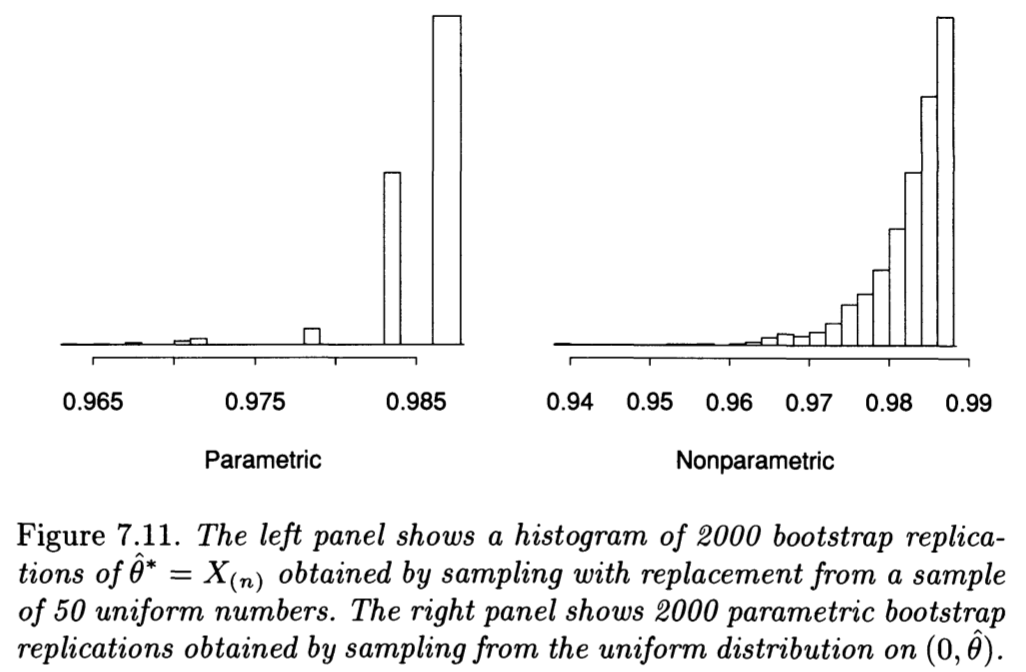
\includegraphics[width=0.9\linewidth]{6/f711.png}
\newline
\setcounter{table}{5} 
Что не так с непарамерическим бутстрепом? Сложность возникает потому, что эмпирическая функция распределения $\hat F$ не является хорошей оценкой настоящего распределения на его краях. Либо параметрические данные о $F$, либо некоторое сглаживание $\hat F$ необходимо для того, чтобы разрешить эту проблему. Детали и ссылки об этой проблеме можно найти в Beran и Ducharme (1991, с.23). Непараметрический бутстреп может отказать и в других примерах, где $\theta$ зависит от гладкости $F.$ К примеру, если $\theta$ есть число атомов у $F$, то $\thetahat = n$ будет плохой оценкой $\thetahat.$ 

\setcounter{chapter}{9}
\chapter{Оценки смещения}
\section{Введение}

Мы сосредоточились на стандартной ошибке как на показателе точности оценки $\hat{\theta}$. Существуют и другие пригодные меры статистической точности (или статистической ошибки), измеряющие различные аспекты поведения оценок  $\hat{\theta}$. В этой главе речь идет о смещении, разнице между ожидаемым значением оценки $\hat{\theta}$ и оцениваемой величиной $\theta$. Алгоритм бутсрепа легко адаптируется для получения оценок смещения, ровно как и для получения оценок стандартной ошибки. Также вводится оценка смещения по методу складного ножа, хотя мы откладываем полное обсуждение метода складного ножа до главы $11$. Можно использовать оценку смещения для исправленной оценки смещения. Однако это может быть опасной практикой, о чем говорится в конце главы.

\section{Бутстреп оценка смещения}

Для начала предположим, что мы вернулись к ситуации с непараметрической выборкой, как в главе 6. Неизвестное распределение вероятностей $F$ дает набор $x = (x_1, x_2 \dots, x_n)$ путем случайной выборки $F \rightarrow x$. Мы хотим оценить вещественный параметр $\theta = t(F)$. Пока возьмем за оценку любую статистику $\hat{\theta} = s(x)$, как показано на рисунке 6.1. Позже нас будет особенно интересовать оценка плагина $\hat{\theta} = t(\hat{F})$.

Смещение $\hat{\theta} = s(x)$ как оценка $\theta$ определяется как разница между математическим ожиданием $\hat{\theta}$ и значением параметра $\theta$,
\begin{equation}\label{eq10.1} 
    \text{bias}_{F} = \text{bias}_{F}(\hat{\theta}, \theta) = E_{F}[s(x)] - t(F).
\end{equation}

Большое смещение обычно является нежелательным аспектом поведения оценки. Мы смирились с тем фактом, что $\hat{\theta}$ является непостоянной оценкой $\theta$, но обычно мы не хотим, чтобы изменчивость была исключительно низкой или высокой. Несмещенные оценки те, для которых $E_{F}(\hat{\theta}) = \theta$, играют важную роль в статистической теории и практике. Они способствуют хорошему чувству научной объективности в процессе оценки. Оценки плагина $\hat{\theta} = t(\hat{F})$ необязательно являются несмещенными, но они, как правило, имеют небольшие смещения по сравнению с величиной их стандартных ошибок. Это одна из хороших черт принципа плагина.

Мы можем использовать бутстреп чтобы вычислить смещение любой оценки $\hat{\theta} = s(x)$. Бутстреп оценка смещения определяется как оценка смещения, которую мы получаем, подставляя $\hat{F}$ вместо $F$ в \ref{eq10.1},
\begin{equation}\label{eq10.2} 
    \text{bias}_{\hat{F}} = E_{\hat{F}}[s(x^{*})] - t(\hat{F}).
\end{equation}

Здесь $t(\hat{F})$ --- оценка плагина $\theta$ может отличаться от $\hat{\theta} = s(x)$. Другими словами, $\text{bias}_{\hat{F}}$ --- это оценка плагина $\text{bias}_{F}$ независимо от того, является ли $\hat{\theta}$ оценкой плагина $\theta$ или нет. Обратите внимание, что $\hat{F}$ используется дважды при переходе от \ref{eq10.1} к \ref{eq10.2}: при замене $F$ в $t(F)$ и при замене $F$ в $E_{F}[s(x)]$.

Если $s(x)$ --- среднее значение, а $t(F)$ --- среднее значение генеральной совокупности, легко показать, что $\text{bias}_{\hat{F}} = 0$. Это имеет смысл, потому что среднее --- это несмещенная оценка среднего для генеральной совокупности, то есть $\text{bias}_{F} = 0$. Однако обычно статистика имеет некоторую систематическую ошибку, и $\text{bias}_{\hat{F}}$ дает оценку этой систематической ошибки. Простым примером является выборочная дисперсия $s(x) = \sum_{1}^n(x_{i} - \Bar{x})^{2}/n$, погрешность которой равна $(-1/n)$ дисперсии генеральной совокупности. В этом случае легко показать, что $\text{bias}_{\hat{F}} = (-1/n^{2})\sum_{1}^n(x_{i} - \Bar{x})^{2}$.

Для большинства статистик, которые возникают на практике, идеальная бутстреп оценка $\text{bias}_{\hat{F}}$ должна быть аппроксимирована моделированием Монте-Карло. Мы генерируем независимую бутстреп выборку $x^{*1}, x^{*2}, \dots x^{*B}$ как на рисунке $6.1$, вычисляем бутстреп репликации $\hat{\theta}^{*}(b) = s(x^{*b})$ и аппроксимируем бутстреп математическое ожидание $E_{\hat{F}}[s(x^{*})]$ средним
\begin{equation}\label{eq10.3} 
    \hat{\theta^{*}}(\cdot) = \sum\limits_{b=1}^{B}\hat{\theta^{*}}(b)/B = \sum\limits_{b=1}^{B} s(x^{*b})/B.
\end{equation}
Бутстреп оценка смещения, основанная на $B$ репликах $\widehat{\text{bias}}_{B}$, есть \ref{eq10.2} с заменой $E_{\hat{F}}[s(x^{*})]$ на $\hat{\theta^{*}}(\cdot)$,
\begin{equation}\label{eq10.4} 
   \widehat{\text{bias}}_{B} = \hat{\theta^{*}}(\cdot) - t(\hat{F}).
\end{equation}
Обратите внимание, что алгоритм, показанный на рисунке $6.1$, точно применяется к вычислению \ref{eq10.4}, за исключением того, что на последнем шаге мы вычисляем $\hat{\theta^{*}}(\cdot) - t(\hat{F})$, а не $\widehat{se}_{B}$. Конечно, мы можем вычислить как $\widehat{se}_{B}$, так и $\widehat{\text{bias}}_{B}$ с помощью того же набора бутстреп репликаций.
\section{Пример: данные об уровне гормона при ношении различных пластырей}

Исторически сложилось так, что статистики очень беспокоились о возможных смещениях в оценках соотношений. Данные об уровне гормона в таблице $10.1$ представляют удобный пример. Восемь субъектов носили медицинские пластыри, предназначенные для введения в кровоток определенного природного гормона. У каждого испытуемого измеряли уровень гормона в крови после ношения трех разных пластырей: пластыря с плацебо, не содержащего гормона, <<старого>> пластыря, произведенного на более старом заводе, и <<нового>> пластыря, произведенного на недавно открывшемся заводе. Первые три столбца таблицы показывают три измерения показателей крови для каждого субъекта.

\noindent
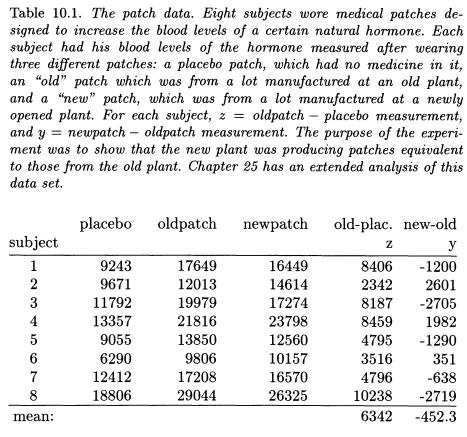
\includegraphics[width=\linewidth]{10/t10.1.png}
\newline

Целью эксперимента с пластырем было показать биоэквивалентность. Пластыри, изготовленные на старом заводе, уже были одобрены для продажи Управлением по санитарному надзору за качеством пищевых продуктов и медикаментов (FDA). Пластыри с нового завода не потребовали полного нового исследования FDA. Их одобрили бы к продаже, если бы можно было доказать, что они биоэквивалентны тем, что были изготовлены на старом заводе. Критерий биоэквивалентности FDA заключается в том, что ожидаемая эффективность новых пластырей соответствует ожидаемой эффективность старых пластырей в том смысле, что
\begin{equation}\label{eq10.5}
    \frac{\left|E(\text{new}) - E(\text{old})\right|}{E(\text{old}) - E(\text{placebo})} \leq .20.
\end{equation}
Другими словами, FDA хочет, чтобы новое лекарство соответствовало старому в пределах $20\%$ количества гормона, которое старый препарат добавляет к <<плацебо>> уровню крови.

Пусть $\theta$ параметр
\begin{equation}\label{eq10.6}
    \theta = \frac{\left|E(\text{new patch}) - E(\text{old patch})\right|}{E(\text{old patch}) - E(\text{placebo patch})}.
\end{equation}
В главах 12--14 рассматриваются доверительные интервалы для $\theta$, подход, который приводит к полному ответу на вопрос о биоэквивалентности: <<действительно ли $|\theta| \leq 0.20$?.>>\footnote{В главе 25 представлен расширенный анализ биоэквивалентности этого набора данных.} Здесь мы рассматриваем только смещение и стандартную ошибку оценки плагина $\hat{\theta}$.

Нас интересуют две статистики, $z_{i}$ и $y_{i}$, полученные для каждого из восьми субъектов,
\begin{equation}\label{eq10.7}
   z = \text{oldpatch measurment} - \text{placebo measurment}
\end{equation}
и
\begin{equation}\label{eq10.8}
   y = \text{newpatch measurment} - \text{oldpatch measurment}.
\end{equation}

Предполагая, что пары $x_{i} = (z_{i}, y_{i})$ получены путем случайной выборки из неизвестного двумерного распределения $F$, $F \rightarrow x = (x_{1}, x_{2} \dots x_{8})$, тогда $\theta$ в \ref{eq10.6} это параметр
\begin{equation}\label{eq10.9}
   \theta = t(F) = \frac{E_{F}(y)}{E_{F}(z)}.
\end{equation}

В этом случае $t(\cdot)$ является функцией, которая принимает распределение вероятностей $F$ на парах $x = (z, y)$ и выдает отношение математических ожиданий. Оценка плагина $\theta$ равна
\begin{equation}\label{eq10.10}
   \hat{\theta} = t(\hat{F}) = \frac{\Bar{y}}{\Bar{z}} = \frac{\sum_{i=1}^{8}y_{i}/8}{\sum_{i=1}^{8}z_{i}/8},
\end{equation}
которую мы возьмем за нашу оценку $\hat{\theta} = s(X)$. Обратите внимание, что ничто в этих формулировках не предполагает, что $z$ и $y$ независимы друг от друга. Последние два столбца таблицы 10.1 показывают $z_{i}$ и $y_{i}$ для восьми испытуемых. Значение $\hat{\theta}$ равно
\begin{equation}\label{eq10.11}
   \hat{\theta} = \frac{-452.3}{6342} = -0.0713.
\end{equation}
Мы видим, что $|\hat{\theta}|$ значительно меньше $0.20$, так что есть некоторая надежда на выполнение условия биоэквивалентности FDA.

На рисунке 10.1 показана гистограмма $B = 400$ бутстреп репликаций $\hat{\theta}$, полученных как в (6.1--6.2): бутстреп выборки $x^{*} = (x_{1}^{*}, x_{2}^{*}, \dots, x_{8}^{*}) =\\=(x_{i_1}, x_{i_2}, \dots, x_{i_8})$ дают бутстреп репликации
\begin{equation}\label{eq10.12}
   \hat{\theta}^{*} = \frac{\Bar{y}^{*}}{\Bar{z}^{*}} = \frac{\sum_{j=1}^{8}y_{i_j}/8}{\sum_{j=1}^{8}z_{i_j}/8}.
\end{equation}

\noindent
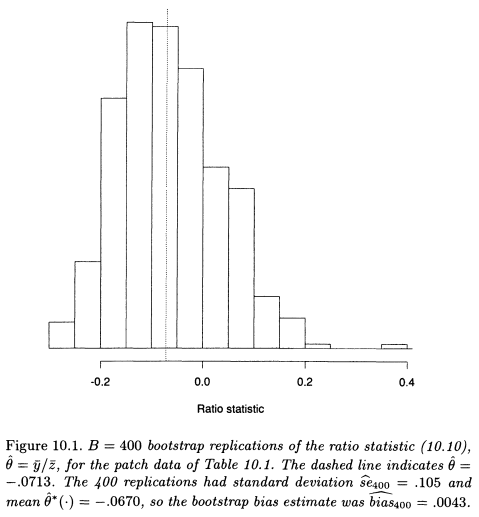
\includegraphics[width=\linewidth]{10/f10.1.png}
\newline

Для $400$ повторов стандартное отклонение выборки составило $\widehat{se}_{400} = 0.105$, а среднее значение выборки $\hat{\theta}^{*}(\cdot) = -0.0670$. Бутстреп оценка смещения составляет
\begin{equation}\label{eq10.12}
   \widehat{\text{bias}}_{400} = -0.0670 - (-0.0713) = 0.0043.
\end{equation}
Это вычисление основано на формуле \ref{eq10.4}, с использованием того факта, что в данном случае $\hat{\theta} = t(\hat{F})$.

Отношение оцененного смещения к стандартной ошибке $\widehat{\text{bias}}_{400}/\widehat{\text{se}}_{400} = 0.041$ мало, что указывает на то, что в этом случае нам не нужно беспокоиться о смещении $\hat{\theta}$. Как правило, смещение меньшее чем $0.25$ стандартных ошибок можно игнорировать, если мы не пытаемся провести аккуратные вычисления доверительных интервалов. Среднеквадратичная ошибка оценки $\hat{\theta}$ для $\theta$ есть $\sqrt{E_{F}\left[(\hat{\theta} - \theta)^{2}\right]}$ мера точности, которая учитывает как смещение, так и стандартную ошибку. Можно показать, что значение среднеквадратичной ошибки равно
\begin{equation*}
   \sqrt{E_{F}\left[(\hat{\theta} - \theta)^{2}\right]} = \sqrt{\text{se}_{F}(\hat{\theta})^{2} + \text{bias}_{F}(\hat{\theta}, \theta)^{2}} =
\end{equation*}
\begin{equation}\label{eq10.14}
   =\text{se}_{F}(\hat{\theta}) \cdot \sqrt{1 + \left(\frac{\text{bias}_{F}}{\text{se}_{F}}\right)^{2}} \doteq \text{se}_{F}(\hat{\theta}) \cdot \left[1 + \left(\frac{\text{bias}_{F}}{\text{se}_{F}}\right)^{2}\right].
\end{equation}
Если $\text{bias}_{F} = 0$, то среднеквадратичная ошибка равна её минимальному значению $\text{se}_{F}$. Если $|\text{bias}_{F}/\text{se}_{F}| < 0.25$, тогда среднеквадратичная ошибка не превосходит $\text{se}_{F}$ больше, чем примерно на $3.1\%$.

Мы знаем, что $B = 400$ бутстреп репликаций обычно более чем достаточно для получения хорошей оценки стандартной ошибки. Достаточно ли этого, чтобы получить хорошую оценку смещения? Ответ в данном конкретном случае --- нет. Помните, что в определении идеальной бутстреп оценки смещения  $\widehat{\text{bias}}_{\infty} = \text{bias}_{\hat{F}}$ \ref{eq10.2},  $\widehat{\text{bias}}_{B}$ \ref{eq10.4} заменяет $E_{\hat{F}}(\hat{\theta}^{*})$ на $\hat{\theta}^{*}(\cdot)$. По распределению бутстреп репликаций мы можем сказать, насколько хорошо $\hat{\theta}^{*}(\cdot)$ оценивает $E_{\hat{F}}(\hat{\theta}^{*})$. Применение 5.6 дает
\begin{equation}\label{eq10.15}
    \text{Prob}_{\hat{F}}\left\{|\hat{\theta}^{*}(\cdot)-E_{\hat{F}}\{\hat{\theta}^{*}\}| < 2\frac{\widehat{\text{se}}_{B}}{\sqrt{B}}\right\}
    = \text{Prob}_{\hat{F}}\left\{|\widehat{\text{bias}}_{B}-\widehat{\text{bias}}_{\infty}| < 2\frac{\widehat{\text{se}}_{B}}{\sqrt{B}}\right\} \doteq 0.95,
\end{equation}
где $\widehat{\text{se}}_{B}$ --- бутстреп оценка стандартной ошибки. Для бутстреп данных на рисунке 10.1 с $\widehat{\text{se}}_{B} = 0.105$ и $B = 400$, мы получаем
\begin{equation}\label{eq10.16}
    \text{Prob}_{\hat{F}}\left\{|\widehat{\text{bias}}_{B}-\widehat{\text{bias}}_{\infty}| < 0.0105\right\} \doteq 0.95,
\end{equation}
большой диапазон погрешности по сравнению с расcчитанным значением $\widehat{\text{bias}}_{400} = 0.0043$.

Граница ошибки $0.0105$ в \ref{eq10.16} достаточно мала, чтобы показать, что смещение здесь не является большой проблемой: так как $\widehat{\text{bias}}_{400} = 0.0043$, мы, вероятно, имеем $|\widehat{\text{bias}}_{\infty}| < 0.0043 + 0.0105 = 0.0148$ и поэтому $|\widehat{\text{bias}}|/\widehat{\text{se}} < 0.0148 / 0.106 = 0.14$. Что довольно меньше, чем эмпирическое граница $0.25$. Однако нам все еще может быть интересно узнать $\widehat{\text{bias}}_{\infty}$ или хорошее приближение к нему и вычислениям \ref{eq10.16}, показывающим что $\widehat{\text{bias}}_{400} = 0.0043$, нельзя доверять. Мы могли бы просто увеличить $B$ (смотри задачу 10.5), но в этом нет необходимости.
\section{Улучшенная оценка смещения}

Оказывается, что существует лучший метод, чем (\ref{eq10.4}), для аппроксимации $\widehat{\text{bias}}_{\infty} = \text{bias}_{\hat{F}}$ из $B$ бутстреп репликаций. Улучшенный метод применяется, когда $\hat{\theta}$ --- это оценка по методу подстановки $t(\hat{F})$ для $\theta = t(F)$. Мы описываем метод здесь и даем объяснение, почему он работает, в главе 23.

Нам нужно определить понятие вектора повторной выборки. Пусть $P_{j}^{*}$ указывает долю бутстреп наблюдений $x^{*} = (x_{1}^{*}, x_{2}^{*}, \dots, x_{n}^{*})$, которая равна $j$-ому исходному наблюдению,
\begin{equation}
    P_{j}^{*} = \#\{x_{j}^{*} = x_{j}\}/n,\quad\quad j = 1, 2, \dots, n.
\end{equation}
Вектор повторной выборки
\begin{equation}\label{eq10.18}
    P^{*} = (P_{1}^{*}, P_{2}^{*}, \dots, P_{n}^{*})
\end{equation}
имеет неотрицательные компоненты в сумме дающие единицу. Например, третья бутстреп выборка для данных об уровне гормона при ношении пластырей была $$X^{*} = (x_1, x_6,x_6, x_5, x_7, x_1, x_3, x_8)$$ и соответствующий вектор повторной выборки $$P^* = (2/8, 0, 1/8, 0, 1/8,2/8, 1/8, 1/8).$$

Бутстреп репликацию $\hat{\theta}^{*} = s(x^{*})$ можно рассматривать как функцию вектора повторной выборки $P^{*}$. Например, если $\hat{\theta} = \bar{y}/\bar{z}$ в (\ref{eq10.10}),
\begin{equation}\label{eq10.19}
   \hat{\theta}^{*} = \bar{y}^{*}/\bar{z}^{*} = \frac{\sum_{i=1}^{8}P^{*}_{j}y_{i}/8}{\sum_{i=1}^{8}P^{*}_{j}z_{i}/8}.
\end{equation}
(Обратите внимание, что исходные данные $x$ считаются фиксированными в этом определении; единственными случайными величинами являются $P_{j}^{*}$.) Для $\hat{\theta} = t(\hat{F})$, оценки метода подстановки $\theta$, запишем
\begin{equation}\label{eq10.20}
   \hat{\theta}^{*} = T(P^{*})
\end{equation}
чтобы определить $\hat{\theta}^{*}$ как функцию вектора повторной выборки.\footnote{Мы обозначаем статистику из метода подстановки двумя способами $\hat{\theta} = s(x) = t(\hat{F})$. Аналогично бутстреп репликации обозначаются $\hat{\theta}^{*} = s(x^{*}) = T(P^{*})$. Три функции $s(\cdot)$, $t(\cdot)$ и $T(\cdot)$ представляют одну и ту же статистику, но рассматриваются как функция в трех разных пространствах.} Формула (\ref{eq10.19}) определяет $T(\cdot)$ для $\hat{\theta} = \bar{y}/\bar{z}$. 

Пусть $P^{0}$ обозначает вектор длины $n$, все элементы которого равны $1/n$,
\begin{equation}\label{eq10.21}
   P^{0} = (1/n, 1/n, \dots, 1/n).
\end{equation}
Значение $T(P^{0})$ --- это значение $\hat{\theta}^{*}$, когда каждый элемент $P_{j}^{*} = 1/n$, то есть когда каждая точка исходных данных $x_j$ встречается ровно один раз в бутстреп выборке $x^{*}$. Это означает, что $x^{*} = x$, за исключением, возможно, перестановок порядка, в котором появляются элементы $x_{1}, x_{2}, \dots, x_{n}$. Но статистика вида $\hat{\theta} = t(\hat{F})$ не меняется, когда элементы $x = (x_1, x_2, \dots, x_n)$ переупорядочиваются, потому что $F$ не изменяется. Другими словами,
\begin{equation}\label{eq10.22}
   T(P^{0}) = \hat{\theta} = t(\hat{F}),
\end{equation}
наблюдаемое выборочное значение статистики. (Это легко проверить в (\ref{eq10.19}).)

$B$ бутстреп выборок $x^{*1}, x^{*2}, \dots, x^{*B}$ приводят к соответствующим векторам повторной выборки $P^{*1}, P^{*2}, \dots, P^{*B}$, каждый вектор $P^{*b}$ имеет форму (\ref{eq10.18}). Определим $\bar{P}^{*}$ как среднее значение этих векторов
\begin{equation}\label{eq10.23}
   \bar{P}^{*} = \sum\limits_{i=1}^{B}P^{*b}/B.
\end{equation}
Согласно (\ref{eq10.22}) мы можем записать бутстреп оценку смещения (\ref{eq10.4}) в виде
\begin{equation}\label{eq10.24}
   \widehat{\text{bias}}_{B} = \hat{\theta}^{*}(\cdot) - T(P^{0}).
\end{equation}
\noindent
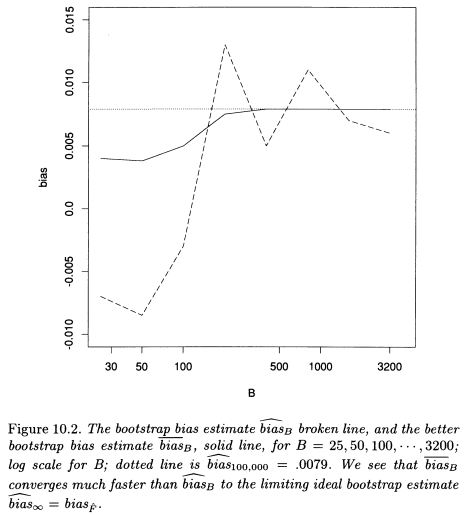
\includegraphics[width=\linewidth]{10/f10.2.png}
\newline
Улучшенная бутстреп оценка смещения, которую мы обозначим как $\overline{\text{bias}}_{B}$, равна
\begin{equation}\label{eq10.25}
   \overline{\text{bias}}_{B} = \hat{\theta}^{*}(\cdot) - T(\bar{P}^{0}).
\end{equation}
Для рисунка 10.1 четыреста векторов повторной выборки усреднены до\\$\bar{P}^{*} =(0.1178, 0.1187, 0.1313, 0.1259, 0.1219, 0.1275, 0.1306, 0.1213)$. Это приводит к
\begin{equation}\label{eq10.26}
  T(\bar{P}^{*}) = \frac{\sum_{i=1}^{8}\bar{P}^{*}_{j}y_{i}}{\sum_{i=1}^{8}\bar{P}^{*}_{j}z_{i}} = -0.0750
\end{equation}
и
\begin{equation}\label{eq10.27}
  \overline{\text{bias}}_{400} = -0.0670 - (-0.0750) = 0.0080,
\end{equation}
в отличие от $\widehat{\text{bias}}_{400} = 0.0043$.

Обе оценки $\widehat{\text{bias}}_{B}$ и $\overline{\text{bias}}_{B}$ сходятся к $\widehat{\text{bias}}_{\infty} = \text{bias}_{\hat{F}}$, идеальной бутстреп оценке смещения, когда $B$ стремится к бесконечности. Для $\overline{\text{bias}}_{B}$ сходимость происходит намного быстрее, поэтому мы назвали её улучшенной. Более быстрая сходимость видна на рисунке 10.2, на котором рассмотрены $\widehat{\text{bias}}_{B}$ и $\overline{\text{bias}}_{B}$ для $B$, равного $25, 50, 100, 200, 400, 800, 1670, 3200$. Предельное значение $\widehat{\text{bias}}_{\infty}$ было аппроксимировано $\widehat{\text{bias}}_{100000}= 0.0079$, показанным пунктирной горизонтальной линией. $\overline{\text{bias}}_{B}$ плавно и быстро приближается к пунктирной линии, в то время как $\widehat{\text{bias}}_{B}$ все еще довольно изменчива даже для $B = 3200$.

В главе 23 обсуждаются улучшенные вычислительные бутстреп методы. Там будет показано, что $\overline{\text{bias}}_{B}$ сводится к использованию $\widehat{\text{bias}}_{CB}$, где $C$ --- большая константа, часто $50$ или больше. %Задача 10.7 предлагает одну причину превосходства $\overline{\text{bias}}_{B}$.
\section{Оценка смещения по методу складного ножа}

Складной нож был оригинальным компьютерным методом оценки смещения и стандартных ошибок. Оценка смещения методом складного ножа, которая кратко обсуждается здесь и более подробно в главе 11, была предложена Морисом Кенуйем в середине 1950-х годов. При наличии набора данных $x = (x_1, x_2, \dots, x_n)$, $i$-я реализация складного ножа $x_{(i)}$ определяется как $x$ с удаленной $i$-й точкой наблюдений,
\begin{equation}\label{eq10.28}
    x_{(i)} = (x_1, x_2, \dots, x_{i-1}, x_{i+1}, \dots, x_n),
\end{equation}
для $i = 1, 2, \dots, n$. Для статистики $\theta = s(x)$ $i$-я репликация складного ножа $\hat{\theta}_{(i)}$~---~это $s(\cdot)$, вычисленная для $x_{(i)}$, предположим
\begin{equation}\label{eq10.29}
    \hat{\theta}_{(i)} = s(x_{(i)}) \quad\quad \text{для}\; i = 1, 2, \dots, n.
\end{equation}
Для статистики метода подстановки $\hat{\theta} = t(\hat{F})$, $\hat{\theta}_{(i)}$ равна $t(\hat{F}_{(i)})$, где $\hat{F}_{(i)}$ --- эмпирическое распределение $n-1$ точек в $x_{(i)}$·

Оценка смещения складного ножа определяется как
\begin{equation}\label{eq10.30}
    \widehat{\text{bias}}_{\text{jack}} = (n-1)\left(\hat{\theta}_{(\cdot)} - \hat{\theta}\right),
\end{equation}
где
\begin{equation}\label{eq10.31}
    \hat{\theta}_{(\cdot)} = \sum\limits_{i=1}^{n}\hat{\theta}_{(i)}/n.
\end{equation}
Эта формула применяется только к статистике метода подстановки $\hat{\theta} = t(\hat{F})$. Формула не работает, если $t(\hat{F})$ --- негладкая статистика, такая как медиана, но для гладкой статистики, такой как $\hat{\theta} = \bar{y}/\bar{z}$ (тех статистик, для которых функция $T(P^{*})$ в (\ref{eq10.20}) дважды дифференцируема) она дает оценку смещения с помощью всего $n$ повторных вычислений функции $t(\cdot)$. Это сравнивается с $B$ повторными вычислениями для будстреп оценок, где $B$ должно быть не менее $200$ даже для $\overline{\text{bias}}_{B}$.

\noindent
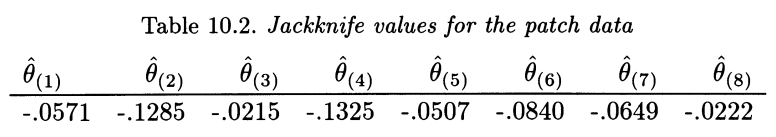
\includegraphics[width=\linewidth]{10/t10.2.png}
\newline

Для данных об уровне гормона статистика отношения $\hat{\theta} = \bar{z}/\bar{y} = -0.0713$ (формула (\ref{eq10.10})), репликации складного ножа показаны в таблице 10.2. Это приводит к $\hat{\theta}_{(\cdot)} = -0.0702$, и
\begin{equation}\label{eq10.32}
    \widehat{\text{bias}}_{\text{jack}} = 7\{-0.0702 - ( -0.0713)\} = 0.0080.
\end{equation}
Не случайно, что $\widehat{\text{bias}}_{\text{jack}}$ так близко согласуется с идеальной бутстреп оценкой $\widehat{\text{bias}}_{\infty} = \widehat{\text{bias}}_{\hat{F}}$. В главе 20 показано, что $\widehat{\text{bias}}_{\text{jack}}$ --- это приближение оценки смещения, полученной по методу подстановки, рядом Тейлора второго порядка. Важно помнить следующее: все три оценки смещения, $\widehat{\text{bias}}_{B},\, \overline{\text{bias}}_{B}$ и $\widehat{\text{bias}}_{\text{jack}}$ пытаются аппроксимировать одну и ту же идеальную оценку $\text{bias}_{\hat{F}}$. В главе 20 обсуждается инфинитезимальный складной нож --- еще один способ приблизительного определения смещения. Мы также увидим аппроксимации, отличные от $\widehat{\text{se}}_{B}$, для идеальной оценки стандартной ошибки $\text{se}_{\hat{F}}$ (хотя здесь сложнее улучшить прямое приближение Монте-Карло $\widehat{\text{se}}_{B}$). Во всех методах численной аппроксимации работает только один принцип оценки, подстановка $\hat{F}$ вместо $F$ в любую меру точности, которую мы хотим оценить. Реализация этого принципа численно эффективным способом --- важная тема, но современные компьютеры настолько мощны, что даже неэффективные способы обычно достаточно хороши, чтобы дать пригодные ответы.

Идеальная оценка $\text{bias}_{\hat{F}}$ имеет недостатки. Если позволить $B \rightarrow \infty$, изменчивость смещения $\widehat{\text{bias}}_{B}$ из-за выборки Монте-Карло устраняется. Однако остается вариабельность $\widehat{\text{bias}}_{\infty} = \text{bias}_{\hat{F}}$ из-за случайности $\hat{F}$ как оценки $F$. Другими словами, у нас все еще есть обычные ошибки, связанные с оценкой любого параметра по выборке.

\noindent
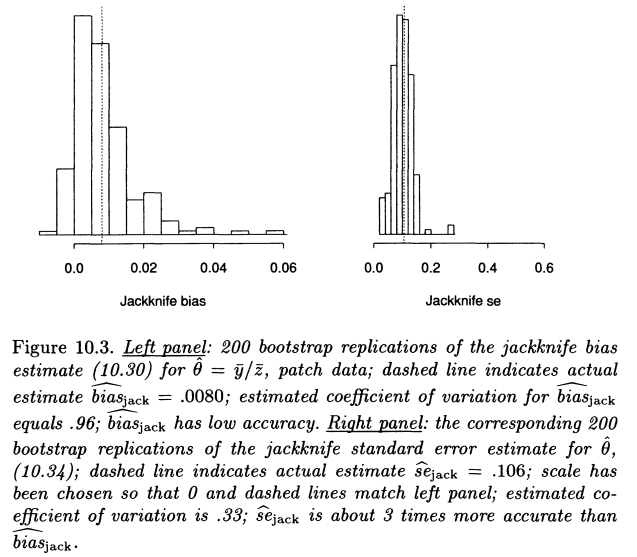
\includegraphics[width=\linewidth]{10/f10.3.png}

Мы могли бы использовать бутстреп для вычисления изменчивости идеальной бутстреп оценки $\text{bias}_{\hat{F}}$, как показано на рисунке 6.1, за исключением практических трудностей вычисления статистики $s(x) = \text{bias}_{\hat{F}}$. Вместо этого давайте рассмотрим более простую статистику $s(x) = \widehat{\text{bias}}_{\text{jack}}$, которая для $\hat{\theta} = \bar{y}/\bar{z}$ обычно близка к $\text{bias}_{\hat{F}}$. Статистика $s(x) = \widehat{\text{bias}}_{\text{jack}}$ является сложной функцией от $x$, требующей сначала вычисления $\hat{\theta}$, затем $\hat{\theta}_{(i)}$ и, наконец, (\ref{eq10.30}), но мы все ещё можем использовать бутстреп для оценки стандартной ошибки $s(x)$.

$B = 200$ бутстреп выборок размера $n = 8$ были сгенерированы из данных об уровне гормона при ношении пластырей, и для каждой выборки была рассчитана оценка смещения по методу складного ножа для статистики отношения, скажем, $\widehat{\text{bias}}_{\text{jack}}^{*}$. Левая часть рисунка 10.3 представляет собой гистограмму из $200$ значений $\widehat{\text{bias}}_{\text{jack}}^{*}$.

Ясно, что статистика $s(x) = \widehat{\text{bias}}_{\text{jack}}$ сильно варьируется. Стандартное отклонение и среднее $200$ репликаций $s(x^{*})$ равнялись соответственно $0.0081$ и $0.0084$, что давало оценку коэффициента вариации 
\begin{equation}\label{eq10.33}
    \widehat{\text{cv}}(\widehat{\text{bias}}_{\text{jack}}) = 0.0081/0.0084 = 0.96.
\end{equation}
Десять процентов значений $\widehat{\text{bias}}_{\text{jack}}^{*}$ были меньше нуля и $16\%$ больше $2\cdot \widehat{\text{bias}}_{\text{jack}} = 0.0160$.

Нет ничего плохого ни в $\widehat{\text{bias}}_{\text{jack}}$, ни в $\text{bias}_{\hat{F}}$. Проблема в том, что $n = 8$ точек данных недостаточно для точного определения смещения статистики отношения в этой ситуации. Рисунок 10.3 поясняет это. Вычисления смещения не были пустой тратой времени. Мы достаточно уверены, что истинное смещение $\hat{\theta} = \bar{y}/\bar{z}$ , каким бы оно ни было, находится где-то между $-0.005$ и $0.025$. Бутстреп стандартная ошибка $\hat{\theta}$ была $0.105$, поэтому отношение абсолютного смещения к стандартной ошибке, вероятно, меньше $0.25$. Вычисление (\ref{eq10.14}) показывает, что в данном случае систематическая ошибка не вызывает особого беспокойства.

Этот расчет предполагает другое беспокойство. Возможно, бутстреп оценка стандартной ошибки $\widehat{\text{se}}_{200} = 0.105$ тоже ненадежна. Теоретически мы могли бы провести бутстреп $\widehat{\text{se}}_{200}$, чтобы выяснить это, но это сложно с вычислительной точки зрения. Однако существует оценка стандартной ошибки по методу складного ножа, предложенная Джоном Тьюки в конце 1950-х годов, которая требует меньше вычислений, чем $\widehat{\text{se}}_{200}$:
\begin{equation}\label{eq10.34}
    \widehat{\text{se}}_{\text{jack}} = \left[\frac{n-1}{n}\sum\limits_{i=1}^{n}\left(\hat{\theta}_{(i)} - \hat{\theta}_{(\cdot)}\right)^{2}\right]^{1/2}.
\end{equation}
Эта формула, которая применяется к гладко определенной статистике, такой как $\hat{\theta} = \bar{y}/\bar{z}$, обсуждается в главе 11. Оказывается, это альтернатива $\widehat{\text{se}}_{B}$ численной аппроксимации идеальной бутстреп оценки $\widehat{\text{se}}_{\infty} = \text{se}_{\hat{F}}(\hat{\theta}^{*})$. Статистика отношения данных об уровне гормона (\ref{eq10.2}) дает
\begin{equation}\label{eq10.35}
   \widehat{\text{se}}_{\text{jack}} = 0.106,
\end{equation}
почти то же самое, что и $\widehat{\text{se}}_{200}$. Мы увидим, что $\widehat{\text{se}}_{\text{jack}}$ не всегда является хорошим приближением к $\widehat{\text{se}}_{\infty}$, но для $\hat{\theta} = \bar{y}/\bar{z}$ это вполне приемлемо.

Те же $200$ бутстреп выборок, использованные для обеспечения репликации $\widehat{\text{bias}}_{\text{jack}}$ на рисунке 10.3, также дали бустреп репликации $\widehat{\text{se}}_{\text{jack}}$. Гистограмма $200$ бутстреп значений  $\widehat{\text{se}}_{\text{jack}}$, показанная на правой части рисунка 10.3, указывает на существенную изменчивость, но не такую большую, как для $\widehat{\text{bias}}_{\text{jack}}$. Гистограмма имеет среднее значение $0.099$ и стандартное отклонение $0.033$, что дает выборочный коэффициент вариации
\begin{equation}\label{eq10.36}
   \widehat{\text{cv}}(\widehat{\text{se}}_{\text{jack}}) = 0.33,
\end{equation}
только треть $\widehat{\text{cv}}(\widehat{\text{bias}}_{\text{jack}})$. На самом деле стандартную ошибку обычно легче оценить, чем смещение, а также она является более важным фактором, определяющим вероятностные характеристики оценки $\hat{\theta}$.

Мы обсудили оценку $\text{bias}_{F}(\hat{\theta}, \theta)$, уравнение (\ref{eq10.1}). Бутсреп процедуру оценки смещения, которая сводится к подстановке $\hat{F}$ вместо $F$ в $\text{bias}_{F}$, можно обобщить: 1) мы можем рассмотреть общие вероятностные механизмы $P \rightarrow x$, как на рисунке 8.3. (Обратите внимание, что здесь <<$P$>> означает нечто иное, чем вектор повторной выборки $P^{*}$, (\ref{eq10.18}).) 2) Мы можем рассмотреть общие меры смещения, $\text{bias}_{P}(\hat{\theta}, \theta)$, например, медианное смещение
\begin{equation}\label{eq10.37}
   \text{bias}_{P}(\hat{\theta}, \theta) = \text{median}_{P}(\hat{\theta}(x)) - \theta(P).
\end{equation}
На рисунке 10.4 показана схема. Идеальная бутстреп оценка $\text{bias}_{P}(\hat{\theta}, \theta)$ это оценка метода подстановки
\begin{equation}\label{eq10.38}
   \text{bias}_{P}(\hat{\theta}^{*}, \theta(\hat{P})).
\end{equation}
Здесь $\hat{P} \rightarrow x^{*}$ --- бутстреп данные; $\hat{\theta}^{*} = s(x^{*})$ --- бутстреп репликация $\hat{\theta} = s(x)$; и $\theta(\hat{P})$~---~значение интересующего параметра $\theta = t(P)$, когда $P=\hat{P}$, механизм оценки вероятности. (Мы не можем писать $\theta(\hat{P}) = \hat{\theta}$, поскольку $t(\cdot)$ может быть другой функцией, отличной от $s(\cdot)$) Для медианного смещения (\ref{eq10.37})
\begin{equation}\label{eq10.39}
   \text{bias}_{\hat{P}}(\hat{\theta}^{*}, \theta(\hat{P})) = \text{median}_{\hat{P}}(\hat{\theta}(x^{*})) - \theta(\hat{P}).
\end{equation}
Обычно $\text{bias}_{\hat{P}}$ нужно аппроксимировать методами Монте-Карло. Усовершенствованные методы, такие как $\overline{\text{bias}}_{B}$ и $\widehat{\text{bias}}_{\text{jack}}$, обычно недоступны для общих мер смещения, таких как (\ref{eq10.37}).
\section{Поправка на смещение}

Зачем нам нужно оценивать смещение $\hat{\theta}$? Обычная причина --- исправить $\hat{\theta}$, чтобы она стала менее смещенной. Если $\widehat{\text{bias}}$ является оценкой смещения $\text{bias}_{F}(\hat{\theta}, \theta)$, то очевидной оценкой с поправкой на смещение является
\begin{equation}\label{eq10.40}
    \bar{\theta} = \hat{\theta} - \widehat{\text{bias}}
\end{equation}
Принимая $\widehat{\text{bias}}$ равным $\widehat{\text{bias}}_{B} = \hat{\theta}^{*}(\cdot) - \hat{\theta}$, получаем
\begin{equation}\label{eq10.41}
    \Bar{\theta} = 2\hat{\theta} - \hat{\theta}^{*}(\cdot).
\end{equation}
(Существует тенденция --- неправильная тенденция --- думать о самой $\hat{\theta}^{*}(\cdot)$ как о скорректированной на смещение оценке. Обратите внимание, что (\ref{eq10.41}) показывает, что если $\hat{\theta}^{*}(\cdot)$ больше $\hat{\theta}$, то исправленная оценка $\Bar{\theta}$ должна быть меньше $\hat{\theta}$.) Положим $\widehat{\text{bias}} = 0.0080$ для статистики отношения данных об уровне гормона при ношении пластырей, равной как $\overline{\text{bias}}_{400}$, так и $\widehat{\text{bias}}_{\text{jack}}$, исправленная оценка отношения $\theta$ равна
\begin{equation}\label{eq10.42}
    \Bar{\theta} = -0.0713 - 0.0080 = -0.0793. 
\end{equation}

На практике исправление смещения может быть опасным. Даже если $\Bar{\theta}$ менее смещена, чем $\hat{\theta}$, она может иметь значительно большую стандартную ошибку. Еще раз, это можно проверить с помощью бутсрепа. Для статистики отношения данных об уровне гормона $200$ бутстреп репликаций $\Bar{\theta} = \hat{\theta} - \widehat{\text{bias}}_{\text{jack}}$ сравнивались с соответствующими репликациями $\hat{\theta}$. Бустреп оценки стандартной ошибки $\bar{\theta}$ и $\hat{\theta}$ были почти идентичны, поэтому в этом случае исправление смещения не было опасным.

\noindent
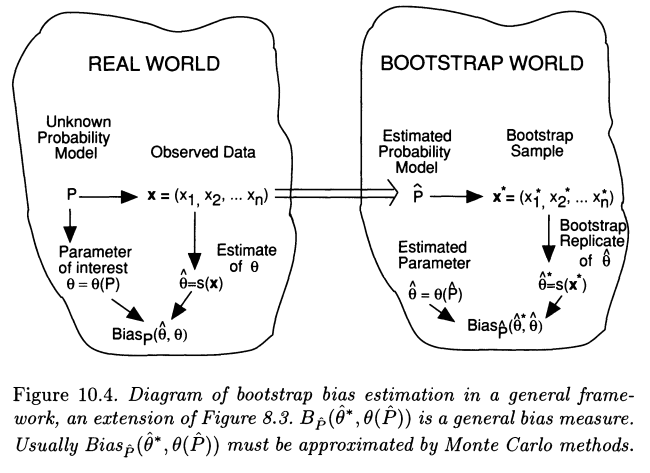
\includegraphics[width=\linewidth]{10/f10.4.png}
\newline

Подводя итог, можно сказать, что оценка смещения обычно интересна и целесообразна, но точное использование оценки смещения часто проблематично. Систематические ошибки оценить труднее, чем стандартные ошибки, как показано на рисунке 10.3. Прямое исправление смещения (\ref{eq10.40}) может быть опасно для использования на практике из-за большой изменчивости $\widehat{\text{bias}}$. Исправление смещения может вызвать большее увеличение стандартной ошибки, что, в свою очередь, приводит к большей среднеквадратичной ошибке (уравнение (\ref{eq10.14})). Если $\widehat{\text{bias}}$ мало по сравнению с предполагаемой стандартной ошибкой $\widehat{\text{se}}$, то безопаснее использовать $\hat{\theta}$, чем $\Bar{\theta}$. Если $\widehat{\text{bias}}$ велико по сравнению с $\widehat{\text{se}}$, то это может указывать на то, что статистика $\hat{\theta} = s(x)$ не является подходящей оценкой параметра $\theta$.

Оценка ошибки предсказания --- одна из важных задач, в которой полезно исправление смещения. Смещение очевидной оценки велико по сравнению со стандартной ошибкой, и его можно эффективно уменьшить, добавив поправочный член. Подробности приведены в главе 17.

\chapter{Метод складного ножа}
\section{Введение}

В главе 10 мы упоминаем складной нож --- метод оценки смещения и стандартной ошибки оценки. Складной нож появился раньше бутстрепа и имеет близкое сходство с ним. В этой главе мы подробно исследуем метод складного ножа. Некоторые из представленных здесь идей получили дальнейшее развитие в главах 20 и 21.
\section{Определение складного ножа}

Предположим, у нас есть выборка $x = (x_1, x_2, \dots, x_n)$ и оценка $\hat{\theta} = s(x)$. Мы хотим оценить смещение и стандартную ошибку $\hat{\theta}$. Складной нож фокусируется на выборках, которые не учитывают одно наблюдение за раз:
\begin{equation}\label{eq11.1}
    x_{(i)} = (x_1, x_2, \dots, x_{i-1}, x_{i+1}, \dots, x_n)
\end{equation}
для $i = 1, 2, \dots, n$, так называемых выборках складного ножа. Выборка складного ножа под номером $i$ состоит из набора данных с удаленным $i$-м наблюдением. Пусть
\begin{equation}\label{eq11.2}
    \hat{\theta}_{(i)} = s(x_{(i)})
\end{equation}
будет $i$-й репликацией складного ножа $\hat{\theta}$.

Оценка смещения по методу складного ножа определяется как
\begin{equation}\label{eq11.3}
   \widehat{\text{bias}}_{\text{jack}} = (n-1)\left(\hat{\theta}_{(\cdot)} - \hat{\theta}\right),
\end{equation}
где
\begin{equation}\label{eq11.4}
   \hat{\theta}_{(\cdot)} = \sum\limits_{i=1}^{n}\hat{\theta}_{(i)}/n.
\end{equation}
Оценка стандартной ошибки по методу складного ножа определяется как
\begin{equation}\label{eq11.5}
   \widehat{\text{se}}_{\text{jack}} = \left[\frac{n-1}{n}\sum\left(\hat{\theta}_{(i)} - \hat{\theta}_{(\cdot)}\right)^{2}\right]^{1/2}.
\end{equation}

Откуда берутся эти формулы? Начнем с $\widehat{\text{se}}_{\text{jack}}$. Вместо того, чтобы смотреть на все (или некоторые) наборы данных, которые могут быть получены путем выборки с заменой из $x_1, x_2, \dots, x_n$, складной нож рассматривает $n$ фиксированных выборок $x_{(1)}, \dots, x_{(n)}$, полученные удалением по одному наблюдению за раз. Подобно бутстреп оценке стандартной ошибки, формула для $\widehat{\text{se}}_{\text{jack}}$ выглядит как стандартное отклонение выборки этих $n$ значений, за исключением того, что первый коэффициент равен $(n-1)/n$ вместо $1/(n-1)$ или $1/n$. Конечно, $(n-1)/n$ намного больше, чем $1/(n-1)$ или $1/n$. Интуитивно этот <<коэффициент увеличения>> необходим, потому что отклонения складного ножа
\begin{equation}\label{eq11.6}
   \left(\hat{\theta}_{(i)} - \hat{\theta}_{(\cdot)}\right)^{2}
\end{equation}
имеют тенденцию быть меньше, чем бутстреп отклонения
\begin{equation}\label{eq11.7}
   \left[\hat{\theta}^{*}(b) - \hat{\theta}^{*}(\cdot)\right]^{2},
\end{equation}
поскольку типичная выборка метода складного ножа больше похожа на исходные данные $x$, чем типичная бутстреп выборка.

Точный вид множителя $(n-1)/n$ получается путем рассмотрения частного случая $\hat{\theta} = \Bar{x}$. Тогда легко показать, что
\begin{equation}\label{eq11.8}
   \widehat{\text{se}}_{\text{jack}} = \left\{\sum\limits_{1}^{n}(x_i-\bar{x})^2/\{(n-1)n\}\right\}^{1/2}.
\end{equation}
То есть коэффициент $(n-1)/n$ --- это именно то, что нужно, чтобы сделать $\widehat{\text{se}}_{\text{jack}}$ равным несмещенной оценке стандартной ошибки среднего. Коэффициент $[(n-1)/n]^2$ приведет оценке метода подстановки
\begin{equation}\label{eq11.9}
   \left\{\sum\limits_{1}^{n}(x_i-\bar{x})^2/n^{2}\right\}^{1/2},
\end{equation}
но это существенно не отличается от несмещенной оценки, если только $n$ не мало. Соглашение о том, что $\widehat{\text{se}}_{\text{jack}}$ использует множитель $(n-1)/n$,  несколько произвольно.

Аналогичным образом, оценка смещения по методу складного ножа (\ref{eq11.3}) кратна среднему значению отклонений складного ножа
\begin{equation}\label{eq11.10}
   \hat{\theta}_{(i)} - \hat{\theta}, \quad i = 1, 2, \dots, n.
\end{equation}
Величины (\ref{eq11.10}) иногда называют величинами влияния складного ножа. Обратите внимание на множитель $(n-1)$ в (\ref{eq11.3}). Это коэффициент увеличения, аналогичный тому, который появляется при оценке по методу складного ножа стандартной ошибки. Чтобы вывести его, мы не можем обратиться к частному случаю $\hat{\theta} = \bar{x}$, потому что $\bar{x}$ несмещенная, а $\hat{\theta}_{(\cdot)} - \hat{\theta}$, как и должно быть, равно нулю. Поскольку этот случай не говорит нам, каким должен быть старший фактор, мы вместо этого рассматриваем в качестве нашего тестового примера выборочную дисперсию
\begin{equation}\label{eq11.11}
   \hat{\theta} = \sum\limits_{1}^{n}(x_{i}-\bar{x})^{2}/n.
\end{equation}
Она имеет смещение $-1/n$ дисперсий генеральной совокупности, а множитель $(n-1)$ перед $\hat{\theta}_{(\cdot)} - \hat{\theta}$ делает $\widehat{\text{bias}}_{\text{jack}}$ равным $-1/n$, умноженному на $$\sum(x_i-\bar{x})^2/(n-1),$$ несмещенной оценке дисперсии генеральной совокупности.

\section{Пример: данные о тестировании}
Давайте применим оценку стандартной ошибки по методу складного ножа к набору данных о результатах тестов $88$ студентов, приведенному в таблице 7.1. Напомним, что представляющая интерес статистика --- это отношение наибольшего собственного значения ковариационной матрицы к сумме собственных значений, как указано в (7.8)
\begin{equation}\label{eq11.12}
    \hat{\theta} = \hat{\lambda}_{1}/\sum\limits_{1}^{5}\hat{\lambda}_{i}.
\end{equation}
Чтобы применить метод складного ножа, мы удаляем по одному каждый случай (строку) в таблице 7.1 и вычисляем $\hat{\theta}$ для каждого набора данных размером $87$. На верхней части рисунка 11.1 показана гистограмма $88$ значений складного ножа $\hat{\theta}_{(i)}$.

Мы также вычислили $88$ бутстреп значений $\hat{\theta}$. Обратите внимание, что разброс гистограммы, полученной с помощью метода складного ножа, намного меньше, чем разброс бутстреп гистограммы, показанной на нижней части рисунка (мы принудительно задаем одну и ту же горизонтальную шкалу во всех гистограммах). Это иллюстрирует тот факт, что наборы данных складного ножа в среднем более похожи на исходный набор данных, чем бутстреп наборы данных. По средне на рисунке показана гистограмма <<завышенных>> значений складного ножа
\begin{equation}\label{eq11.13}
    \sqrt{87}\left(\hat{\theta}_{(i)} - \hat{\theta}_{(\cdot)}\right)
\end{equation}
с разрывом в точке среднего складного ножа $\hat{\theta}_{(\cdot)}$. С этим <<коэффициентом увеличения>> гистограмма складного ножа похожа на бутсреп гистограмму, показанную на нижней части рисунка. Величина $\widehat{\text{se}}_{\text{jack}}$ оказывается равной $0.049$, что лишь немного больше, чем значение $0.047$ для бутстреп оценки, полученной в главе 7.
\section{Псевдо-значения}

Другой способ думать о складном ноже --- это псевдо-значения
\begin{equation}\label{eq11.14}
    \widetilde{\theta}_{i} = n\hat{\theta} - (n-1)\hat{\theta}_{(i)}.
\end{equation}
Обратите внимание, что в частном случае $\hat{\theta} = \Bar{x}$, мы имеем $\widetilde{\theta}_{i} = x_{i}$, $i$-е значение данных. Кроме того, для любой $\hat{\theta}$ формула для $\widehat{\text{se}}_{\text{jack}}$ может быть выражена как
\begin{equation}\label{eq11.15}
    \widehat{\text{se}}_{\text{jack}} = \left\{\sum\limits_{1}^{n}\left(\tilde{\theta}_{i} - \tilde{\theta}\right)^2/\{(n-1)n\}\right\}^{1/2},
\end{equation}
где $\Tilde{\theta} = \sum\tilde{\theta}_{i}/n$. Это похоже на оценку стандартной ошибки среднего для <<данных>> $\tilde{\theta}_{i},\; i = 1, 2, \dots, n$. Идея, лежащая в основе \ref{eq11.14}, состоит в том, что псевдо-значения должны действовать так, как если бы они были $n$ независимыми значениями.

Что произойдет, если мы попытаемся продолжить эту идею и использовать псевдо-значения для построения доверительного интервала? Один из разумных подходов --- сформировать интервал
\begin{equation}\label{eq11.16}
    \widetilde{\theta} \pm t_{n-1}^{(1-\alpha)}\widehat{\text{se}}_{\text{jack}},
\end{equation}

\noindent
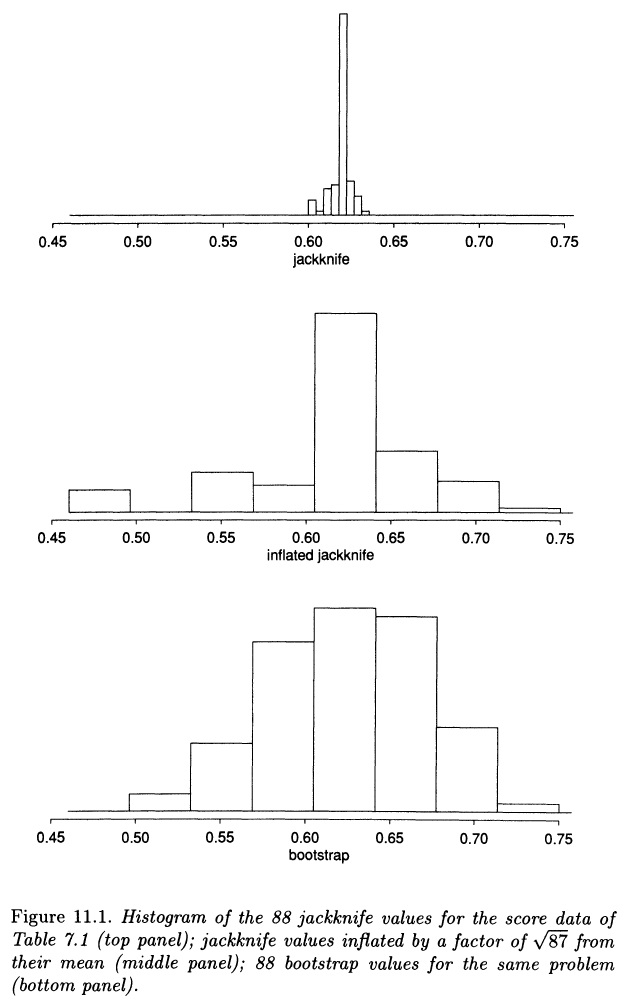
\includegraphics[width=\linewidth]{11/f11.1.jpg}
\newline

\noindentгде $t_{n-1}^{(1-\alpha)}$ --- $(1-\alpha)$-й процентиль распределения $t$ c $n-1$ степеням свободы. Оказывается, этот интервал работает не очень хорошо: в частности, он ненамного лучше, чем более грубые интервалы, основанные на теории о нормальном распределении. Для построения доверительного интервала необходимы более совершенные подходы, как описано в главах 12–14. Хотя псевдо-значения интригуют, неясно, являются ли они хороший способ думать о складном ноже. Мы не будем здесь их рассматривать.
\section{Связь метода складного ножа и бутстрепа}

Что лучше, бутстреп или складной нож? Поскольку для этого требуется вычисление $\hat{\theta}$ только для $n$ наборов данных складного ножа, складной нож будет легче вычислить, если $n$ будет меньше, чем, скажем, $100$ или $200$ репликаций, используемых бутстрепом для оценки стандартной ошибки. Однако, рассматривая только $n$ выборок складного ножа, складной нож использует только ограниченную информацию о статистике $\hat{\theta}$, и, таким образом, можно предположить, что складной нож менее эффективен, чем бутстреп. Фактически оказывается, что складной нож можно рассматривать как приближение к бутстрепу. Это объясняется в главе 20. Вот суть идеи: рассмотрим линейную статистику, то есть статистику, которую можно записать в виде
\begin{equation}\label{eq11.17}
    \hat{\theta} = s(x) = \mu + \frac{1}{n}\sum\limits_{1}^{n}\alpha(x_{i}),
\end{equation}
где $\mu$ --- константа, а $\alpha(\cdot)$ --- функция. Среднее --- это простой пример линейной статистики, для которой $\mu = 0$ и $\alpha(x_i) = x_i$. Теперь для такой статистики, оказывается, что оценка по методу складного ножа и бутстреп оценка стандартных ошибок совпадают, за исключением незначительного множителя $\left\{(n-1)n\right\}^{1/2}$, используемого в определении складного ножа. Это именно то, что мы нашли для $\hat{\theta} = \bar{x}$: складной нож дает оценку стандартной ошибки $$\left\{\sum\limits_{1}^{n}(x_{i} - \bar{x})^2/\{(n-1)n\}\right\}^{1/2}$$ в то время как бутстреп приводит к этому значению, умноженному на $\left\{(n-1)n\right\}^{1/2}$. Неудивительно, что для линейной статистики нет потери информации при использовании складного ножа, поскольку знание линейной статистики для $n$ наборов данных складного ножа $x_{(i)}$ определяет значение $\hat{\theta}$ для любого бутстреп набора данных $x^{*}$.

При нелинейной статистике происходит потеря информации. Складной нож линейно аппроксимирует бутстреп: то есть он согласуется с бутстрепом (за исключением множителя $\left\{(n-1)n\right\}^{1/2}$) для некоторой линейной статистики вида (\ref{eq11.17}), которая приближает $\hat{\theta}$. Детали этой интересной взаимосвязи приведены в главе 20. С практической точки зрения, эти результаты показывают, что точность оценки стандартной ошибки по методу складного ножа зависит от того, насколько $\hat{\theta}$ близка к линейности. Для сильно нелинейных функций складной нож может быть неэффективным, а иногда и опасным.

На рисунке 11.2 показаны результаты исследования этой неэффективности на конкретном примере. Мы сгенерировали $200$ выборок размером $10$ из двумерной нормальной совокупности с нулевым средним, единичной дисперсией и корреляцией $0.7$. Ящики с усами слева показывают оценки, полученные по методам бутстреп и складного ножа, стандартной ошибки для $\hat{\theta} = \Bar{x}$, а справа --- для коэффициента корреляции. Горизонтальные линии показывают истинную стандартную ошибку $\hat{\theta}$ в каждом случае. В обоих случаях бутстреп и складной нож демонстрируют небольшое смещение при оценке стандартной ошибки. Вариабельность оценки складного ножа немного больше, чем у бутстрепа для среднего (линейная статистика), но значительно больше для коэффициента корреляции (нелинейная статистика). По этой причине в последнем случае предпочтительнее использовать бутстреп. %Задача 11.13 рассматривает бутстреп и  метод складного ножа для другой нелинейной статистики.

\noindent
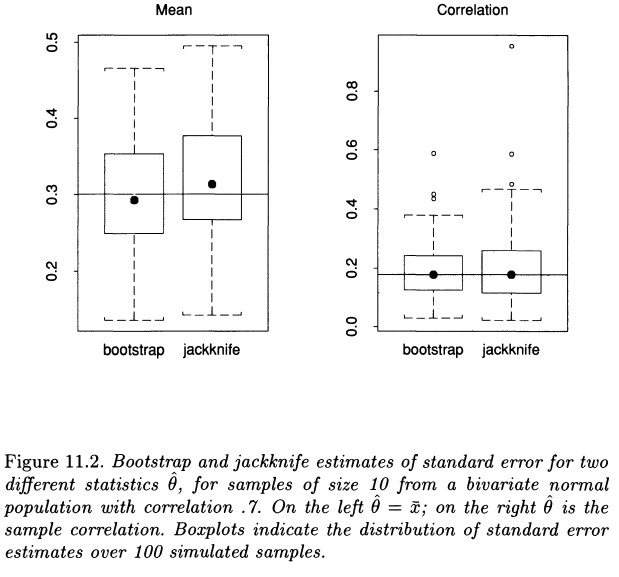
\includegraphics[width=\linewidth]{11/f11.2.png}
\newline

Точно так же можно показать, что оценка смещения складного ножа является приближением к начальной оценке смещения. Приближение в терминах квадратичной (а не линейной) статистики, которая имеет вид
\begin{equation}\label{eq11.18}
    \hat{\theta} = s(x) = \mu + \frac{1}{n}\sum\limits_{1 \leq i \leq n}\alpha(x_i) + \frac{1}{n^2}\sum\limits_{1 \leq i < j \leq n}\beta(x_i, x_j).
\end{equation}
Простым примером квадратичной статистики является выборочная дисперсия (\ref{eq11.11}). Расписывая ее, мы обнаруживаем, что ее можно выразить в форме уравнения (\ref{eq11.18}). Для такой статистики, если мы знаем значение $\hat{\theta}$ для $x$, а также $x_{(i)}, i = 1,2, \dots, n$, мы можем вывести значение $\hat{\theta}$ для любого бутстреп набора данных. Оценки смещения складного ножа и бутстрепа по существу совпадают для квадратичной статистики.
\section{Отказ складного ножа}

Подводя итог, можно сказать, что складной нож часто обеспечивает простое и хорошее приближение к бутстрепу для оценки стандартных ошибок и смещения. Однако, как вкратце упоминалось в главе 10, складной нож может с треском выйти из строя, если статистика $\hat{\theta}$ не является «гладкой». Интуитивно идея гладкости заключается в том, что небольшие изменения в наборе данных вызывают только небольшие изменения в статистике. Простым примером негладкой статистики является медиана. Чтобы понять, почему медиана не является гладкой, рассмотрим $9$ упорядоченных значений из контрольной группы данных о мышах (таблица 2.1):
\begin{equation}\label{eq11.19}
    10,27,31,40,46,50,52,104,146.
\end{equation}
Медиана этих значений равна $46$. Теперь предположим, что мы начинаем увеличивать значение $4$-го по величине значения $x = 40$. Медиана не меняется вообще, пока $x$ не станет больше $46$, а затем после этого медиана будет равна $x$ , пока $x$ не превысит $50$. Это означает, что медиана не является дифференцируемой (или гладкой) функцией от $x$.

Это отсутствие гладкости приводит к тому, что оценка стандартной ошибки по методу складного ножа несовместима с медианой. Для данных о мышах значения складного ножа для медианы\footnote{Медиана четного числа точек данных --- это среднее двух значений из середины.} равны
\begin{equation}\label{eq11.20}
    48,48,48,48,45,43,43,43,43.
\end{equation}
Обратите внимание, что встречаются только $3$ различных значения, что является следствием недостаточной гладкости медианы и того факта, что наборы данных складного ножа отличаются от исходного набора данных только на одно наблюдение. Итоговая оценка $\mathrm{se}_{\mathrm{jack}}$ составляет $6.68$. Для данных о мышах бутстреп оценка стандартной ошибки на основе бутстреп выборок объема $B = 100$ составляет $9.58$, что значительно больше, чем значение складного ножа, равное $6.68$. При $n \rightarrow \infty$, можно показать, что $\mathrm{se}_{\mathrm{jack}}$ противоречива, то есть не может сходиться к истинной стандартной ошибке. С другой стороны, бутстреп рассматривает наборы данных, которые менее похожи на исходный набор данных, чем наборы данных складного ножа, и, следовательно, согласованы с медианой. 
\section{Метод складного ножа с отбрасыванием d наблюдений}
Есть способ исправить несоответствие складного ножа негладкой статистике. Вместо того чтобы исключать по одному наблюдению за раз, мы не учитываем $d$ наблюдений, где $n = r \cdot d$ для некоторого целого числа $r$. Можно показать, что если $n^{1/2}/d \rightarrow \infty$ и $n-d \rightarrow \infty$, то складной нож «с отбрасыванием» согласован с медианой. Грубо говоря, нужно исключить более $d = \sqrt{n}$, но менее $n$ наблюдений, чтобы добиться согласованности в оценке стандартной ошибки складным ножом. Пусть $\hat{\theta}_{(s)}$ обозначает $\hat{\theta}$, примененную к набору данных с удаленным подмножеством $s$. Формула для оценки стандартной ошибки складным ножом с отбрасыванием $d$ наблюдений:
\begin{equation}\label{eq11.21}
    \left\{\frac{r}{\binom{n}{d}}\sum(\hat{\theta}_{(s)} - \hat{\theta}_{(\cdot)})^2\right\}^{1/2},
\end{equation}
где $\hat{\theta}_{(\cdot)} = \sum\hat{\theta}_{(s)}/\binom{n}{d}$ и сумма ведется по всем подмножествам $s$ размера $n - d$, выбранным без замены из $x_1, x_2, \dots, x_n$.

В нашем примере с $n = 9$ мы можем выбрать $d = 4> \sqrt{9}$, и вычисление складного ножа delete-d включает в себя нахождение медианы для
\begin{equation}\label{eq11.22}
    \binom{9}{4} = 126
\end{equation}
выборок, соответствующих одновременному исключению $4$ наблюдений. Это дает оценку стандартной ошибки $7.16$, что несколько ближе к бутстреп значению $9.58$, чем значение складного ножа с удалением одного элемента, которое равно $6.68$.

Если $n$ велико и $\sqrt{n} < d < n$, количество выборок складного ножа $\binom{n}{d}$ может быть очень значительным. Вместо вычисления $\hat{\theta}$ для всех этих подмножеств можно вместо этого охватить случайную выборку подмножеств, что, в свою очередь, сделает складной нож delete-d больше похожим на бутстреп. Текущая работа над складным ножом delete-d представляет собой возрождение исследований складного ножа.

Функция складного ножа на языке $S$ описана в приложении.

\setcounter{chapter}{13}
\chapter{Улучшенные бутстреп-доверительные интервалы}
\section{Введение}
Одной из основных целей теории бутстрепа является автоматическое создание хороших доверительных интервалов. <<Хорошо>> означает, что бутстреп интервалы должны быть близки к точным доверительным интервалам в тех особых ситуациях, когда статистическая теория дает точный ответ, и должны иметь надежные вероятности покрытия в любых ситуациях. Ни метод бутстреп-t главы 12, ни метод процентилей главы 13 не соответствуют этим критериям. Бутстреп-t интервалы имеют хорошие теоретические вероятности покрытия, но на практике имеют тенденцию быть неустойчивыми. Процентильные интервалы более устойчивы, но имеют менее удовлетворительные свойства покрытия.

В этой главе обсуждается улучшенная версия процентильного метода, называемого $\bca$ (аббревиатура, bias–corrected and accelerated). Интервалы $\bca$ являются существенным улучшением по сравнению с процентильными интервалами как в теоретическом плане, так и на практике. Они близки к приведенным выше критериям качества, хотя точность их покрытия все еще может быть неустойчивой для небольших размеров выборки. (Возможны улучшения, как показано в главе 25.) Простой компьютерный алгоритм под названием \texttt{bcanon} производит интервалы $\bca$, затрачивая для этого немного больше усилий, чем для процентильных интервалов. Мы также обсудим метод под названием $\abc$ (аббревиатура, approximate bootstrap confidence intervals) который значительно уменьшает объем вычислений, необходимых для интервалов $\bca$. Глава заканчивается применением этих методов к реальной задаче.
\section{Пример: данные о пространственном восприятии}

Следующий пример, основанный на данных о пространственном восприятии, показывает необходимость улучшения процентильного метода и метода бутстреп-t. Каждый из двадцати шести детей с неврологическими дефектами проходил два теста на пространственное восприятие, тест <<A>> и тест <<B>>. Эти данные показаны в таблице 14.1 и представлены графически на рис. 14.1.

\noindent
\begin{center}
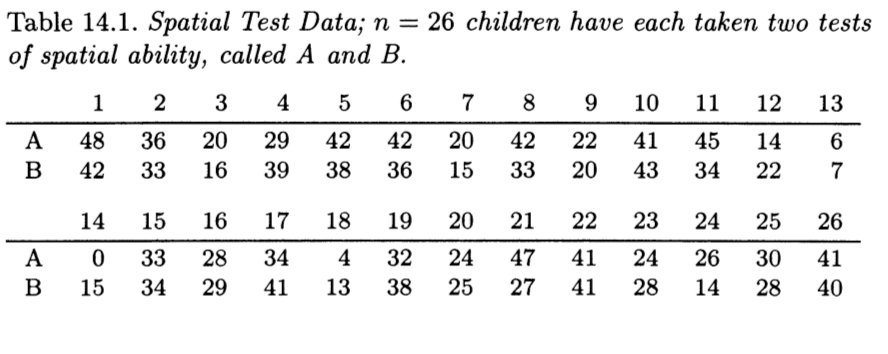
\includegraphics[width=0.9\linewidth]{14/t141.png}
\end{center}
\setcounter{table}{1}

Предположим, что мы хотим найти 90\% доверительный интервал для $\theta = \text{var} (A)$, дисперсии результата теста <<A>>.

Оценка $\theta$ по методу подстановки основана на $n=26$ парах $x_i = (A_i, B_i)$ из таблицы 14.1.
\begin{equation}
	\thetahat = \summ{i = 1}{n} (A_i - \bar A)^2/n = 171.5, \qquad (\hat A = \summ{i = 1}{n} A_i/n)
\end{equation}
\setcounter{equation}{1}
Следует заметить, что это немного меньше обычной несмещенной оценки~$\theta$,
\begin{equation}
	\bar\theta = \summ{i = 1}{n} (A_i - \bar A)^2/(n-1) = 178.4
\end{equation}
\setcounter{equation}{2}
Оценка методом подстановки $\thetahat$ смещена вниз. Метод $\bca$ автоматически делает поправку на смещение в оценке по методу подстановки, что является одним из его достоинств перед процентильным методом.\footnote{Для рассуждений в этой части, а также для алгоритмов \texttt{bcanon} и \texttt{abcnon}, предполагаем, что статистика имеет форму $\thetahat = t(\hat F)$ (получена методом подстановки)}
Гистограмма 2000 бутстреп репликаций $\thetahat^*$ показана на левой панели рисунка 14.2. Репликации получены таким же образом, как и в случае рисунка 6.1: если $\mathbf x = (\xes{26})$ представляет из себя исходный набор данных таблицы 14.1, где $x_i = (A_i,B_i)$, $\ies{26}$, тогда бутстреп выборка $\mathbf x^* = (\xest{26})$ есть случайная выборка размера 26 с возвращением из набора $\{\xes{26}\}$; бутстреп репликация $\thetahat^*$ есть дисперсия А компонент $\bf x^*$, где $x_i^* = (A_i^*, B_i^*),$
\begin{equation}
	\thetahat = \summ{i = 1}{n} (A_i^* - \bar A^*)^2/n, \qquad (\hat A^* = \summ{i = 1}{n} A_i^*/n).
\end{equation}
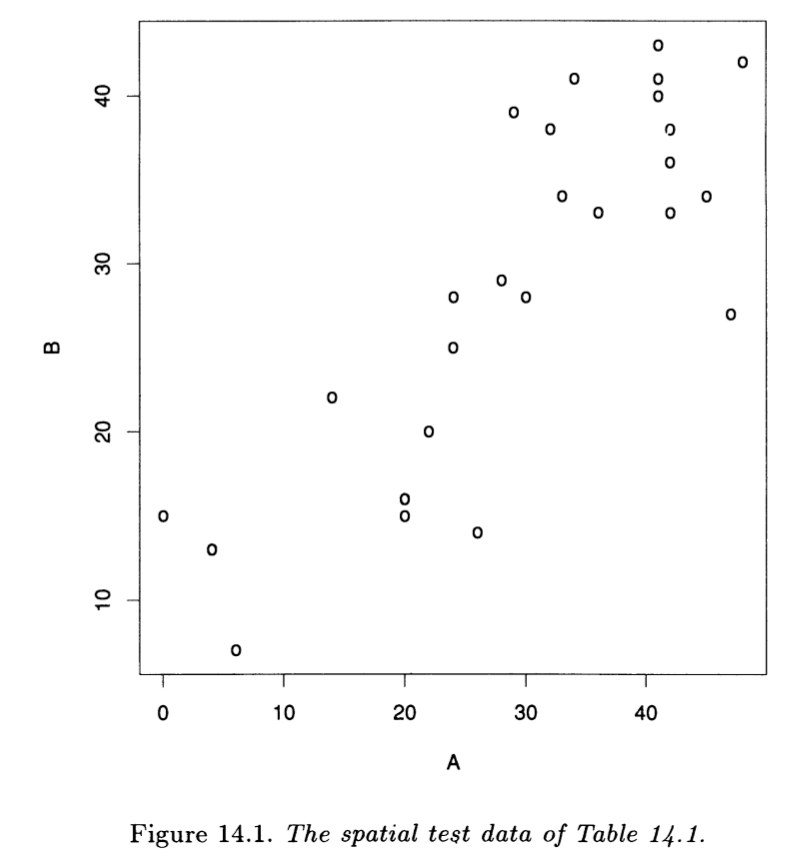
\includegraphics[width=0.85\linewidth]{14/f141.png}
\newline
$B = 2000$ бутстреп выборок $\mathbf x$ дают 2000 бутстреп репликаций $\thetahat^*$ на рис.14.2.\footnote{легко проверить, что нам не нужны вторые компоненты $x_i^*$ для этих вычислений} Это так называемые \textit{непараметрические} бутстреп репликации, которые мы уже рассматривали в предыдущих частях. Далее мы также обсудим \textit{параметрические} бутстреп репликации, а именно предположим нормальную модель для данных. Согласно обозначениям главы 6, непараметрическая бутстреп выборка генерируется случайным выбором из $\widehat F$,
\begin{equation}
	\widehat F \rightarrow \mbf x^* = (\xest{n}),
\end{equation}
\setcounter{equation}{4}
где $\what F$ есть эмпирическая функция распределения, для которого вероятность каждого из $x_i$ равна $1/n$.

В верхней части таблицы 14.2 показаны пять различных приближенных $90\%$ непараметрических доверительных интервалов для $\theta$: 
\begin{itemize}
	\item стандартный интервал $\what \theta \pm 1.645\what \sigma$;
	\item бутстреп оценка стандартной ошибки;
	\item процентильный интервал $(\what \theta^{*(0.05)}, \what \theta^{*(0.95)})$, построенный на основе левой гистограммы на рис. 14.2;
	\item $\bca$ и $\abc$ интервалы, которые обсуждаются в следующих двух разделах;
	\item бутстреп-t интервалы из главы 12. 
\end{itemize}

\noindent
\begin{center}
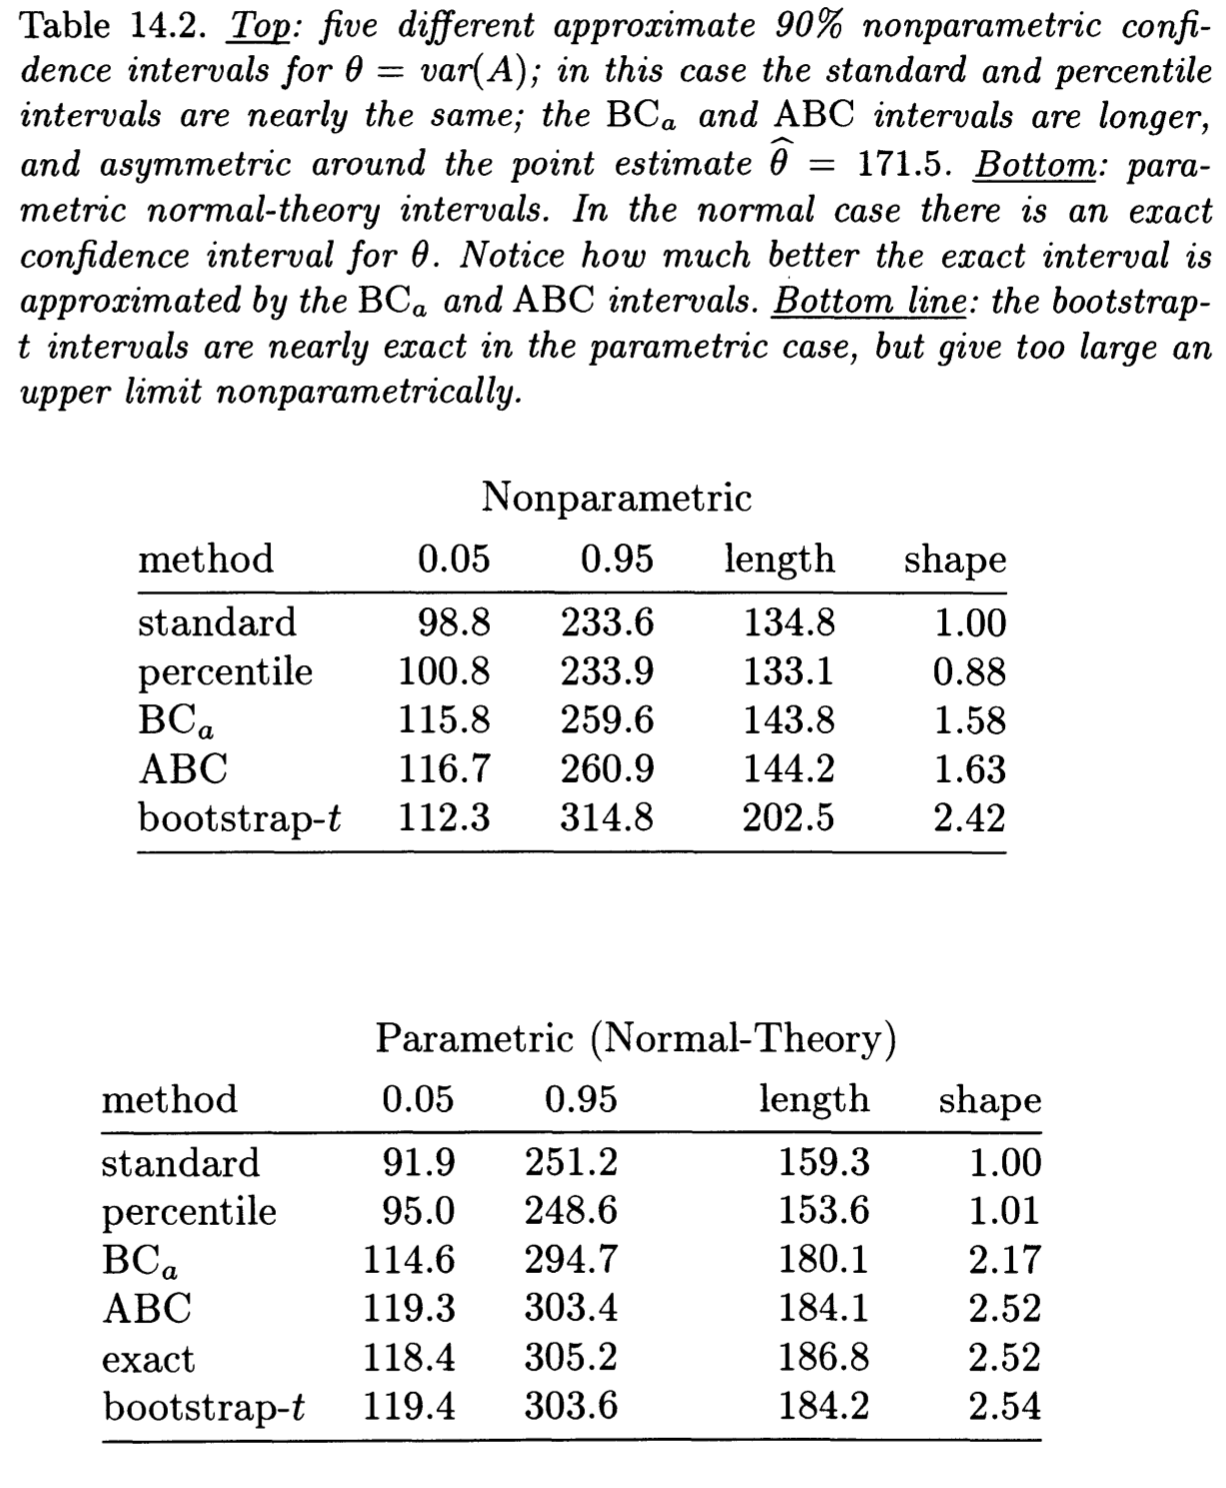
\includegraphics[width=0.9\linewidth]{14/t142.png}
\end{center}
\setcounter{table}{2}
Каждый из интервалов $(\what \theta_\tx{lo}, \what \theta_\tx{up})$ определяется своей длиной и формой (shape):
\begin{equation}
	\tx{length} = \what \theta_\tx{up} - \what \theta_\tx{lo}, \qquad \tx{shape} = \frac{\what{\theta}_\tx{up} - \what{\theta}}{\what{\theta} - \what{\theta}_\tx{lo}}.
\end{equation}
<<Форма>> есть показатель асимметричности интервала относительно оценки $\what \theta$. Показатель формы больший, чем 1, означает, что расстояние между $\what{\theta}$~и~$\what{\theta}_\tx{up}$ больше, чем расстояние между $\what{\theta}$ и $\what{\theta}_\tx{lo}$. Стандартные интервалы симметричны относительно $\what \theta$, откуда $\tx{shape} = 1$ по определению. Точные интервалы, когда они существуют, чаще всего оказываются асимметричными. Построенные стандартные интервалы оказываются ошибочными во-многом из-за их <<врожденной>> симметрии. 

Для рассматриваемого набора данных стандартные и процентильные интервалы практически совпадают. Оба несколько отличаются от $\bca$ и $\abc$ интервалов, которые оказались более длинными и асимметричными вправо относительно $\what \theta$. Общий результат, приведенный в разделе 13.2, говорит о том, что интервалы $\bca$ и $\abc$ лучше, однако мы не можем утверждать об этом однозначно, так как для таких сравнений не существует <<золотого стандарта.>>

В то же время, мы можем получить <<золотой стандарт>>, если рассмотрим задачу оценивания $\tx{var} (A)$ в рамках параметрического подхода (предположив гауссовость\footnote{На самом деле, не похоже, что исходные данные распределены нормально. Однако это не запрещает провести сравнительный анализ методов, аппроксимирующих точный интервал \textit{в предположении}, что данные распределены нормально. Все же, если сравнивать параметрические и непараметрические интервалы, то последние оказываются более предпочтительными для данного набора данных.}). Для этого мы предположим, что результаты тестов $x_i = (A_i, B_i)$ есть случайная выборка из двумерного нормального распределения $F_\tx{norm},$
\begin{equation}
  F_\tx{norm} \rightarrow \mbf x = (\xes{n}).
\end{equation}
При выбранном параметрическом подходе мы можем построить точный доверительный интервал для $\theta = \tx{var} (A)$. %См. задачу 14.4
Этот интервал, названный <<точным>> (\textit{exact}) в таблице 14.2, является <<золотым стандартом>> для оценки различных приближенных интервалов в параметрических условиях.
Выборка гауссового параметрического бутстрепа получается генерацией выборок из двумерного нормального распределения $\what F_\tx{norm}$, которое наилучшим образом соответствует данным $\mbf x$ вместо эмпирического распределения $\what F$, то есть
\begin{equation}
  \what F_\tx{norm} \rightarrow \mbf x^* = (\xest{n}).
\end{equation}
%См. задачу 14.3.
Получив $\mbf x^*$, бутстреп репликация $\what \theta^*$ будет равна 
$$
\summ{1}{n} (A_i^* - \bar A^*)^2/n,
$$
как в (14.3). 

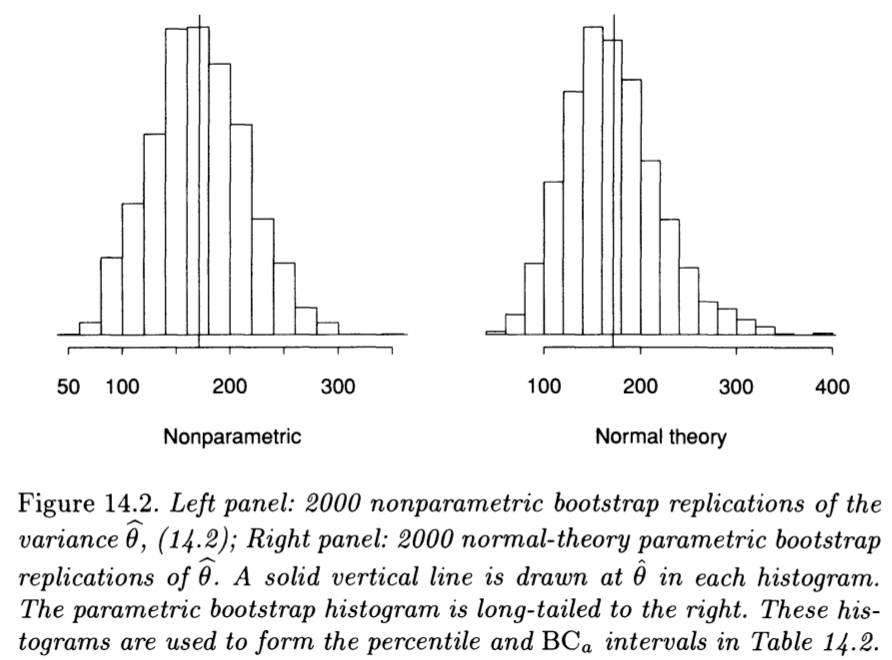
\includegraphics[width=0.85\linewidth]{14/f142.png}
\newline
\noindent Правая гистограмма на рис. 14.2 --- гистограмма 2000 репликаций параметрического бутстрепа. Если сравнить ее с непараметрической версией, гистограмма \textit{normal theory} имеет длинный хвост справа, а также шире, при этом $\what \sigma = 47.1$, если сравнить со стандартной ошибкой в непараметрическом случае --- 41.0.

Если обратить внимание на нижнюю часть таблицы 14.2, то можно увидеть, что интервалы по методам $\bca$ и $\abc$ оказываются близкими к точному <<золотому стандарту>>. И это не просто случайность или частный случай. На самом деле, теория бутстрепа, приведенная кратко в разделе 14.3, говорит о том, что мы можем ожидать успешные результаты от $\bca$ и $\abc$.

Бутстреп-t интервалы для $\theta$ показаны в нижних частях таблицы 14.2. Они основаны на 1000 бутстреп репликаций статистики (по аналогии с $t$-статистикой) $(\what \theta - \theta)/\what{\tx{se}}$, со знаменателем, <<взятым>> из стандартной статистической теории,
\begin{equation}
  \what{\tx{se}} = \left[ \frac{U_4 - U_2^2}{26}  \right]^{1/2} \qquad (U_h = \summ{i = 1}{26} (A_i - \bar A)^h/26).
\end{equation}

Результирующие интервалы, как в (12.19), оказываются практически точными в случаях нормальной теории. Однако верхний предел непараметрического интервала кажется слишком большим, хотя об этом сложно утверждать в отсутствии непараметрического <<золотого стандарта>>. На данном уровне развития метод бутстреп-t не может быть рекомендован к использованию в непараметрической постановке.

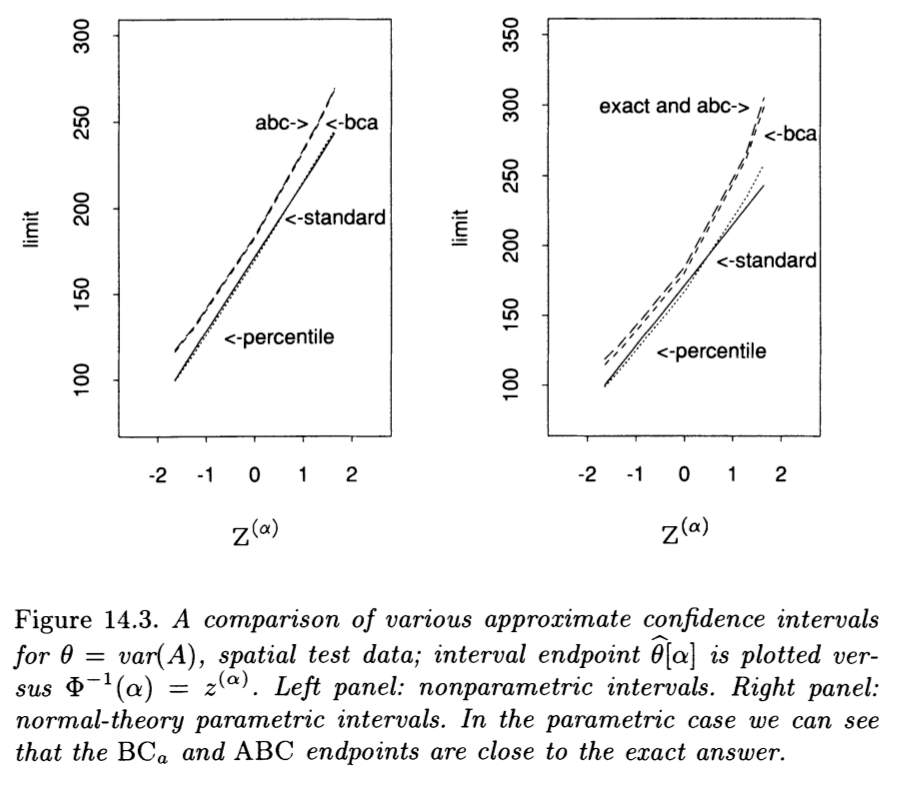
\includegraphics[width=0.85\linewidth]{14/f143.png}
\newline



\section{Метод $\bca$}

В этом разделе описано построение $\bca$ интервалов. Они оказываются более сложными в описании, чем процентильные интервалы, однако в применении они так же просты. Алгоритм \texttt{bcanon}, данный в приложении, строит непараметрические $\bca$ интервалы адаптивно.

Пусть $\what \theta^{*(\alpha)}$ обозначает $100\cdot \alpha$ процентиль $B$ бутстреп репликаций $$\what\theta^*(1),\what\theta^*(2),\ldots,\what\theta^*(B),$$ как в (13.5). Процентильный интервал $(\what \theta_\tx{lo}, \what \theta_\tx{up})$ предполагаемого покрытия $1-2\alpha$, получается напрямую из этих процентилей, то есть
$$
\tx{процентильный метод: } \quad (\what \theta_\tx{lo}, \what \theta_\tx{up}) = 
(\what \theta^{*(\alpha)}, \what \theta^{*(1 - \alpha)}).
$$
Например, пусть $B = 2000$ и $\alpha = 0.05$; тогда процентильный интервал $(\what \theta^{*(0.05)}, \what \theta^{*(0.95)})$ будет интервалом, покрывающим упорядоченные значения $\what \theta^*(b)$ от 100го до 1900го.

Границы интервала $\bca$ также даются процентилями бутстреп распределения, однако они необязательно совпадают с интервалом на основе (14.8). Используемые процентили зависят от двух чисел $\hat a$ и $\hat z_0$, которые определены как \textit{ускорение} (acceleration) и \textit{поправка смещения} (bias-correction), соответственно. Далее мы опишем получение чисел $\hat a$ и $\hat z_0$, но сначала дадим определение границ интервала $\bca$.

\textit{$\bca$ интервал с предполагаемым покрытием $1-2\alpha$ задается парой значений}
\begin{equation}
  	\bca\, : \, (\what \theta_\tx{lo}, \what \theta_\tx{up}) = 
(\what \theta^{*(\alpha_1)}, \what \theta^{*(\alpha_2)}),
\end{equation}
\textit{где}
\begin{align}
	\alpha_1 &= \Phi \left(\hat z_0 + \frac{\hat z_0 + z^{(\alpha)}}{1 - \hat a (\hat z_0 + z^{(\alpha)})}\right), \notag \\
	 \alpha_2 &= \Phi \left(\hat z_0 + \frac{\hat z_0 + z^{(1 -\alpha)}}{1 - \hat a (\hat z_0 + z^{(1 -\alpha)})}\right).
\end{align}
Здесь $\Phi(\cdot)$ есть функция стандартного нормального распределения, a $z^{(\alpha)}$ есть $100\alpha$ процентиль стандартного нормального распределения. К примеру, $z^{(0.95)} = 1.645$ и $\Phi(1.645) = 0.95$.

Формула (14.10) выглядит сложно, однако её легко вычислить. Заметим, что если приравнять $\hat a$ и $\hat z_0$ к нулю, то 
\begin{equation}
  \alpha_1 = \Phi(z^{\alpha}) = \alpha \quad \tx{и} \quad \alpha_1 = \Phi(z^{1-\alpha}) = 1-\alpha,
\end{equation}
откуда можно увидеть, что в таком случае $\bca$ интервал (14.9) совпадает с процентильным интервалом (13.4). Ненулевые значения $\hat a$ или $\hat z_0$ изменяют процентили, используемые для вычисления границ $\bca$. Такие изменения исправляют некоторые недостатки стандартного и процентильного методов, что объясняется в 22 главе.
Непараметрические $\bca$ интервалы из таблицы 14.2 построены на значениях
\begin{equation}
  (\hat a, \hat z_0) = (0.061, 0.146),
\end{equation}
что приводит к значениям (согласно (14.10))
\begin{equation}
  (\alpha_1, \alpha_2) = (0.110,0.985).
\end{equation}
В данном случае $90\%$ $\bca$ интервал есть $
(\what \theta^{*(0.110)}, \what \theta^{*(0.985)})$, интервал, расположенный между 220-ым и 1970-ым  упорядоченными значениями 2000 чисел $\what \theta^* (b)$.

Как вычисляются $\hat a$ и $\hat z_0$? Значение поправки смещения $\hat z_0$ получается напрямую из доли бутстреп репликаций, меньших исходной оценки $\what \theta$,
\begin{equation}
  \hat z_0 = \Phi^{-1} \left(\frac{\#\left\{\what\theta^*(b) < \what \theta\right\}}{B}\right),
\end{equation}
где $\Phi^{-1}(\cdot)$ есть обратная функция к функции распределения стандартного нормального закона.\footnote{то есть $\Phi^{-1}(0.95) = 1.645$} У левой гистограммы на рисунке 14.2 1116 из 2000 значений $\what \theta^*$ оказались меньше, чем $\what \theta = 171.5$, откуда $\hat z_0 = \Phi^{-1}(0.558) = 0.146$. Грубо говоря, $\hat z_0$ оценивает медианное смещение $\what \theta^*$, то есть степень различия между медианой $\what \theta^*(b)$ и $\what \theta$ в <<нормальной>> шкале. Мы получим $\hat z_0$, если ровно половина из всех значений $\what \theta^*(b)$  окажется меньшими или равными $\what \theta$.

Есть несколько способов вычисления ускорения $\hat a$. Проще всего описать его с помощью значений по методу складного ножа статистики $\what \theta = s(\mbf x)$. Пусть $\mbf x_{(i)}$ --- исходная выборка с удаленным наблюдением $x_i$, также обозначим $\what \theta _{(i)} := s(\mbf x_{(i)})$  и $\what \theta_{(\cdot)} = \summ{i = 1}{n} \what \theta_{(i)}/n$, согласно рассуждениям из начала главы 11. Простое выражение для ускорения
\begin{equation}
  \hat a = \frac{\summ{i = 1}{n}\left(\what \theta_{(\cdot)} - \what \theta_{(i)}\right)^3}{6 \left\{\summ{i = 1}{n}\left(\what \theta_{(\cdot)} - \what \theta_{(i)}\right)^2\right\}^{3/2}}.
\end{equation}
У статистики $s(\mbf x) = \summ{i=1}{n} (A_i - \bar A)^2/n$, из (14.2), значение $\hat a$ для набора данных о тестах на пространственное восприятие соатавляет $\hat a = 0.061$. Как $\hat a$, так и $\hat z_0$ вычисляются автоматически реализацией непараметрического алгоритма $\bca$. Величина $\hat a$ называется \textit{ускорением} из-за того, что она описывает скорость изменения стандартной ошибки $\what \theta$ относительно истинного значения параметра $\theta$. Стандартная нормальная аппроксимация --- $\what \theta \sim N(\theta, \tx{se}^2)$ --- предполагает, что стандартная ошибка $\what \theta$ одинакова для всех $\theta$. Однако часто это предположение нереалистично, и константа ускорения $\hat a $ делает поправку. Например, в текущем примере, где $\what \theta$ есть дисперсия, в контексте теории нормального распределения ясно, что $\tx{se} \what \theta \sim \theta$ %(Задача 14.4)
Фактически, $\hat a $ есть скорость изменения стандартной ошибки $\hat \theta$ относительно истинного значения параметра $\theta$, измеренная в <<нормальной>> шкале. Не является очевидным то, почему формула (14.15) должна привести к оценке ускорения стандартной ошибки: некоторые разъяснения этого результата можно найти у Efron (1987).

У метода $\bca$ есть два важных теоретических преимущества. Во-первых, этот метод сохраняет отображения,\footnote{Данное утверждение будет строго верным, если принять другое определение $\hat a$, основанное на конечных разностях, как в главе 22. На практике это различие оказывается несущественным} как в формуле (13.10). Это означает, что граничные точки интервала $\bca$ отображаются корректно при замене интересующего параметра $\theta$ на некоторую функцию от него. Например, $\bca$ интервалы для $\sqrt{\tx{var}(A)}=\sqrt{\theta}$ получаются взятием квадратных корней из граничных точек $\bca$ в таблице 14.2. Свойство сохранения интервала при отображении оберегает от сомнений, которые имеют место при выборе масштаба для бутстреп-t интервала, как в разделе 12.6. $\bca$ автоматически выбирает наилучшую шкалу.

Второе преимущество метода $\bca$ заключается в его точности. Доверительный интервал $(\what \theta_\tx{lo}, \what \theta_\tx{up})$ уровня $1 - 2\alpha$  должен иметь вероятность $\alpha$ \textit{непокрытия} истинного значения $\theta$ сверху или снизу, то есть
\begin{equation}
  \prob{\theta < \what \theta_\tx{lo}} \dot =\, \alpha \quad \tx{ и }  \quad  \prob{\theta > \what \theta_\tx{up}} \dot =\, \alpha
\end{equation}
Можно оценить качество приближенных доверительных интервалов на основании того, насколько они удовлетворяют (14.16). Можно показать, что интервалы $\bca$ имеют второй порядок точности. Это означает, что отклонение от (14.16) сходится к нулю со скоростью $1/n$, (с увеличением размера выборки $n$) то есть 
\begin{equation}
  \prob{\theta < \what \theta_\tx{lo}} \dot =\, \alpha + \frac{c_\tx{lo}}{n} \quad \tx{ и }  \quad  \prob{\theta > \what \theta_\tx{up}} \dot =\, \alpha + \frac{c_\tx{up}}{n}
\end{equation}
для двух констант $c_\tx{lo}$ и $c_\tx{up}$. Стандартный и процентильный методы имеют лишь \textit{первый порядок точности}, поэтому ошибки оказываются на порядок выше:
\begin{equation}
    \prob{\theta < \what \theta_\tx{lo}} \dot =\, \alpha + \frac{c_\tx{lo}}{\sqrt n} \quad \tx{ и }  \quad  \prob{\theta > \what \theta_\tx{up}} \dot =\, \alpha + \frac{c_\tx{up}}{\sqrt n},
\end{equation}
где константы $c_\tx{lo}$ и $c_\tx{up}$ могут отличаться от тех, которые были ранее. Разница между первым и вторым порядком точности имеет не только теоретический характер. Она также приводит к улучшенной аппроксимации точных границ тогда, когда они существуют, как в таблице 14.2.

Метод бутстреп-t имеет второй порядок точности, однако не обладает свойством сохранения отображения. Процентильный метод обладает, однако не имеет второй порядок точности; как и стандартный метод. $\bca$ метод обладает обоими преимуществами. На текущий момент метод $\bca$ рекомендуется к универсальному использованию, в особенности для непараметрических задач. Нельзя сказать, что метод идеален или не может быть модифицирован: в разделе 25.6 главы 25 используется дополнительное применение бутстрепа для улучшения результатов, полученных  с помощью $\bca$ и $\abc$ методов. % В задаче 14.13 о трудностях, которые могут возникнуть с $\bca$ интервалами в экстремальных ситуациях.

Стандартный вызов функции \texttt{bcanon} имеет вид
\begin{equation}
  \texttt{bcanon}(\texttt{x}, \texttt{nboot}, \texttt{theta}),
\end{equation}
где \texttt{x} --- данные, \texttt{nboot} --- число бутстреп репликаций, \texttt{theta} --- вид статистики $\what \theta$. Больше подробностей --- в приложении.


 


\section{Метод $\abc$}
Главный недостаток метода $\bca$ заключается в необходимости проведения большого числа итераций. В главе 19 показано, что для удовлетворительного уменьшения ошибки Монте-Карло требуется не менее $B = 1000$ репликаций. Метод $\abc$ (\textit{approximate bootstrap confidence}) представляет из себя метод, который оценивает границы интервалов аналитически, без использования репликаций Монте-Карло. Данная аппроксимация обычно оказывается достаточно неплохой, что видно из результатов в таблице 14.2. (Разница между граничными точками $\bca$ и $\abc$ объясняется вариативностью Монте-Карло при вычислении $\bca$ интервала. Увеличение $B$ до $10000$ параметрических репликаций дает $\bca$ интервал $(118.4,303.8)$, практически совпадающий с $\abc$ интервалом.)

Метод $\abc$ описан в главе 22. Его работа заключается в аппроксимации результатов бутстреп моделирования используя разложения Тейлора.  Для этого необходимо, чтобы оцениваемая статистика $\what \theta = s(\mbf x)$ была гладкой по $\mbf x$. Пример негладкой статистики --- выборочная медиана. Для большинства часто встречающихся статистик метод $\abc$ оказывается весьма удовлетворительным. (Контрпример приведен в разделе 14.5.) Построенные по $\abc$ интервалы --- как и граничные точки по методу $\bca$  --- сохраняют отображения и имеют второй порядок точности. Для построения оценок по методу $\abc$ в таблице 14.2 потребовалось всего $3\%$  вычислительных затрат, необходимых для построения $\bca$ интервала.

Непараметрические границы по методу $\abc$ в таблице 14.2 были получены из алгоритма \texttt{abcnon}, приведенном в приложении. Для использования этого алгоритма статистика $\what \theta$ должна быть представлена в специальной форме (\textit{resampling form}). Как будет показано в главе 20, эта форма важна для развития теории бутстреп методов. Форма была определена в разделе 10.4. Фиксировав исходную выборку $\mbf x = (\xes{n}),$ запишем бутстреп значение $\what \theta^* = s(\mbf x^*)$ как функцию вектора повторной выборки $\mbf P^*$, то есть
\begin{equation}
  \what \theta^* = T(\mbf P^*).
\end{equation}
Вектор $\mbf P^* = (P_1^*, P_2^*, \ldots, P_n^*)$ состоит из долей
\begin{equation}
  P_i^* = N_i^*/n = \frac{\#\{x_j^*> x_i\}}{n} \qquad (i = \ies{n}).
\end{equation}

Статистика $\what \theta^* = \sum_{i = 1}^{n} (A_i^* - \bar A^*)^2/n$, (14.3), может быть представлена в виде (14.20) следующим образом
\begin{equation}
  \what \theta ^* = \sum_{i = 1}^n P_i^* (A_i - \bar A^*)^2, \tx{ где} \quad \bar A^* = \summ{i =1}{n} P_i^* A_i. 
\end{equation}
Функция $T(\mbf P^*)$ из (14.20) есть необходимая форма статистики, которая используется в алгоритме $\abc$. Напомним,  определен и следующий вектор повторной выборки
\begin{equation}
  \mbf P^0 = (1/n,1/n,\ldots,1/n)
\end{equation}
для которого выполняется $T(\mbf P^0) = \what \theta$, исходное значение статистики. Алгоритм \texttt{abcnon} требует, чтобы  $T(\mbf P^*)$ была гладкой для $\mbf P^*$ в окрестности $\mbf P^0$. Это происходит естественным образом, как в (14.22), для статистик по методу подстановки $\what \theta = t(\what F)$.

Типичный вызов функции \texttt{abcnon} имеет вид
\begin{equation}
  \texttt{abcnon}(\texttt x, \texttt{tt}), 
\end{equation}
где \texttt x --- данные, \texttt{tt} --- статистика $\what \theta ^*$ в специальной форме. Больше информации --- в приложении.

Подводя итоги, $\abc$ интервалы сохраняют отображения, имеют второй порядок точности, а также служат хорошим приближением $\bca$ интервалов для крупного класса гладких статистик $\what \theta^* = s(\mbf x^*)$. Для реализации \texttt{abcnon} алгоритма $\abc$ требуется, чтобы статистика была приведена в специальной форме $\what \theta^* = T(\mbf P^*)$.  В то же время, удобная и простая реализация, а также серьезные вычислительные преимущества указывают на пригодность данного подхода.

\section{Пример: данные о твердости зубов}

\footnote{Материал этого раздела является продвинутым, поэтому он может быть пропущен при первом прочтении}
Мы завершаем эту главу рассмотрением более сложного примера, который покажет как возможности, так и ограничения непараметрических $\bca$ и $\abc$ доверительных интервалов.

В таблице 14.3 можно увидеть данные о твердости зубов. Тринадцать человек, попавших в некоторые происшествия потеряли от одного до четырех здоровых зубов. Твердость удалённых зубов была оценена деструктивным исследованием, что в стандартных условиях неосуществимо. <<Твердость>> в последнем столбце таблицы 14.3 --- измеренный для каждого пациента показатель средней твердости зубов (в логарифмической шкале).

\noindent
\begin{center}
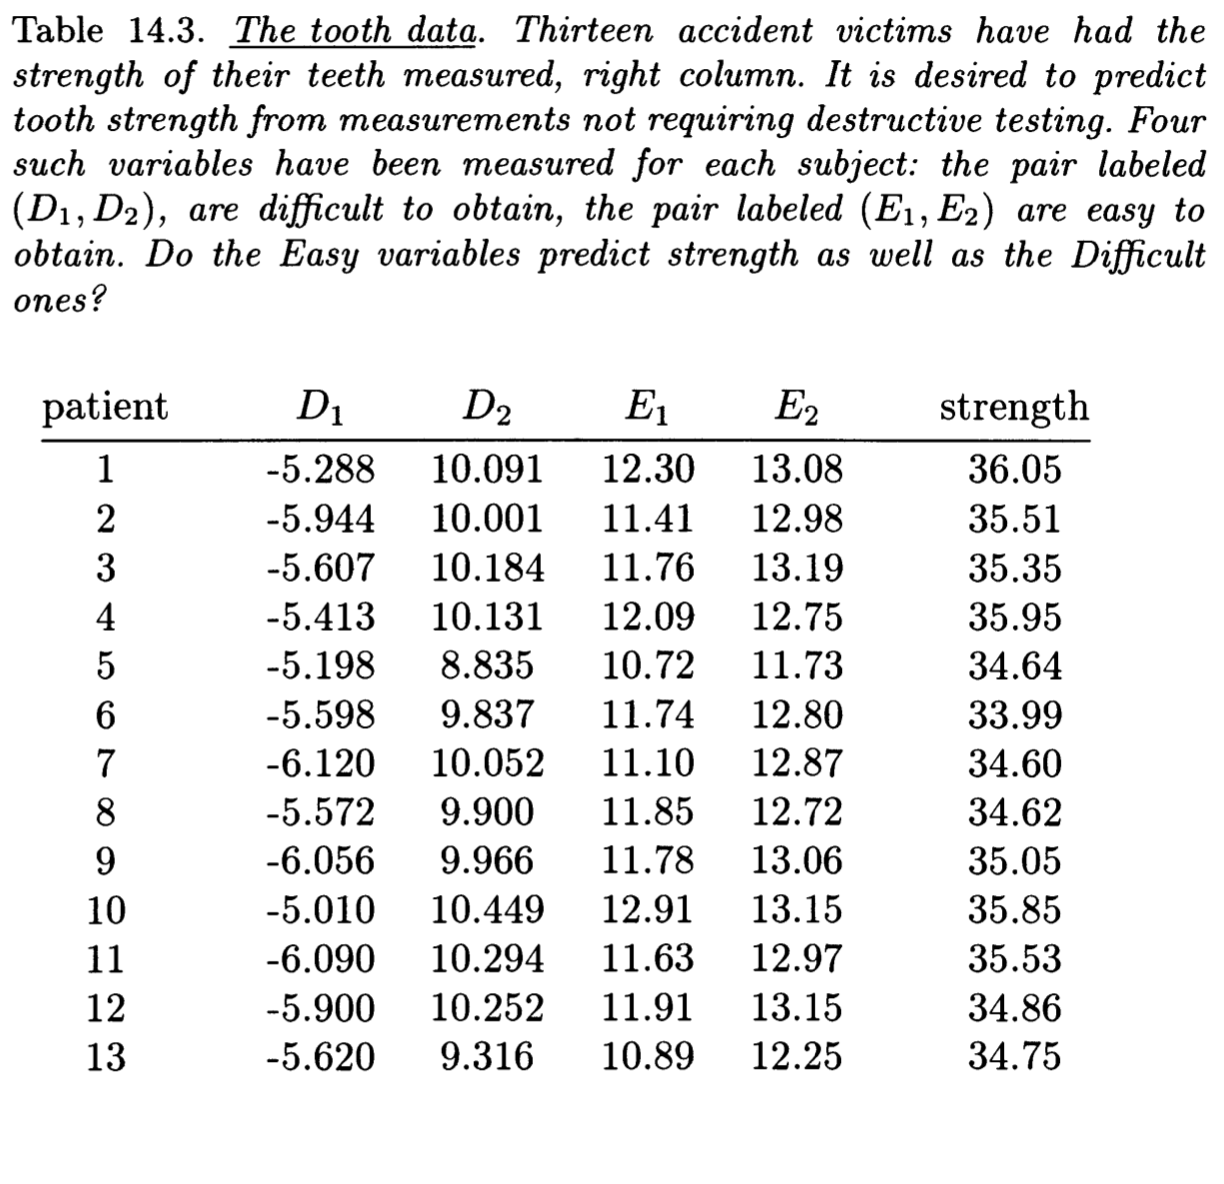
\includegraphics[width=0.9\linewidth]{14/t143.png}
\end{center}
\setcounter{table}{3}

Исследователи хотели предсказать твердость зубов используя переменные, которые не требуют разрушения зубов и могут быть измерены на рутинных осмотрах. В таблице 14.3 показаны данные о четырех таких переменных --- $D_1$, $D_2$, $E_1$, $E_2$. Пару $(D_1, D_2)$ трудно и дорого получить, а пару $(E_1, E_2)$ --- легко и дешево. Исследователи задались следующим вопросом: насколько хорошо <<простые>> переменные $(E_1, E_2)$ предсказывают твердость зубов в сравнении с <<труднодоступными>> $(D_1, D_2)$.

Данный вопрос можно формализовать используя линейные модели, как в главах 7 и 9. Каждая строка $x_i$ матрицы данных из таблицы 14.3 состоит из пяти чисел: двух $D$, двух $E$, а также значения твердости, то есть
\begin{equation}
  x_i = (d_{i1}, d_{i2}, e_{i1}, e_{i2}, y_i) \qquad (i = \ies{13}).
\end{equation}
Пусть $\mbf D$ --- матрица, использующая только переменные $D$ для предсказания $y_i$ с помощью линейной регрессии (включая сдвиг), то есть $\mbf D$ --- матрица $13 \times 3$ с $i$-й строкой вида
\begin{equation}
  (1, d_{i1}, d_{i2}).
\end{equation}

Оценка $y_i$ по методу наименьших квадратов на основе переменных $D$ имеет вид
\begin{equation}
  \what y_i(D) = \what \beta_0(D) + \what \beta_1(D) d_{i1} + \what \beta_2(D) d_{i2},
\end{equation}
где вектор $\what \beta (D) = (\what \beta_0(D),\what \beta_1(D) , \what \beta_2(D))$ есть решение задачи наименьших квадратов
(9.28), то есть
\begin{equation}
  \what \beta (D) = (\mbf D^\mathrm{T} \mbf D)^{-1} \mbf D^\mathrm{T}\mbf y,
\end{equation}
где $y = (y_1,y_2,\ldots,y_{13})$. $\tx{RSE}(D)$ (residual squared error) есть сумма квадратов ошибок между предсказаниями $\what y_i (D)$ и наблюдениями $y_i$ для $n = 13$ пациентов
\begin{equation}
  \tx{RSE}(D) = \summ{i=1}{N} (y_i - \what y_i (D))^2.
\end{equation}
Меньшие значения $\tx{RSE}$ являются индикатором хорошего качества предсказания; наилучшее возможное значение $\tx{RSE} = 0$ достигается на идеальном предсказании для каждого из пациентов.

Аналогичнным образом мы можем предсказывать $y_i$, используя только переменные $E$ и в результате вычислить
\begin{equation}
  \tx{RSE}(E) = \summ{i = 1}{n}(y_i - \what y_i(E))^2.
\end{equation}
Вопрос исследователя о том, насколько переменные двух разных типов, $D$ и $E$, сравнимы по качеству предсказания, может быть переформулирован как вопрос о сравнении \tx{RSE}(D) и \tx{RSE}(E). Практичная в атком случае статистика имеет вид
\begin{equation}
  \what \theta = \frac{1}{n} [\tx{RSE}(E) - \tx{RSE}(D)].
\end{equation}
Положительное значение $\what \theta$ означало бы, что переменные $E$ хуже чем переменные $D$ в предсказании твердости. (Если бы число измерений $E$ и $D$ не совпадают, то статистика $\what \theta$ должна быть преобразована). %см. задачу 14.12 
Были получены значения $\tx{RSE}(D) = 2.761$ и $\tx{RSE}(E) = 3.130$, что приводит к
\begin{equation}
  \what \theta = 0.0285.
\end{equation}
Это свидетельствует о том, что переменные $D$ являются более предпочтительными для предсказания, так как $\what \theta$ больше нуля, однако мы не можем быть уверены в этом, пока не оценим статистическую изменчивость $\what \theta$. Для этого мы используем методы $\bca$ и $\abc$. Рисунок 14.4 указывает на то, что ситуация может оказаться <<пограничной>>, так как предсказанные значения $\what y_i(D)$ и $\what y_i(E)$ близки для каждого из наблюдений. Также следует заметить, что разница между $\tx{RSE}(D)$ и $\tx{RSE}(E)$ составляет около $10\%$ от самих значений $\tx{RSE}$. Поэтому даже если эта разница статистически значима, она может быть не сильно важной в практическом плане. Построение доверительного интервала позволит ответить как на вопрос значимости, так и на вопрос важности этой разницы.
 

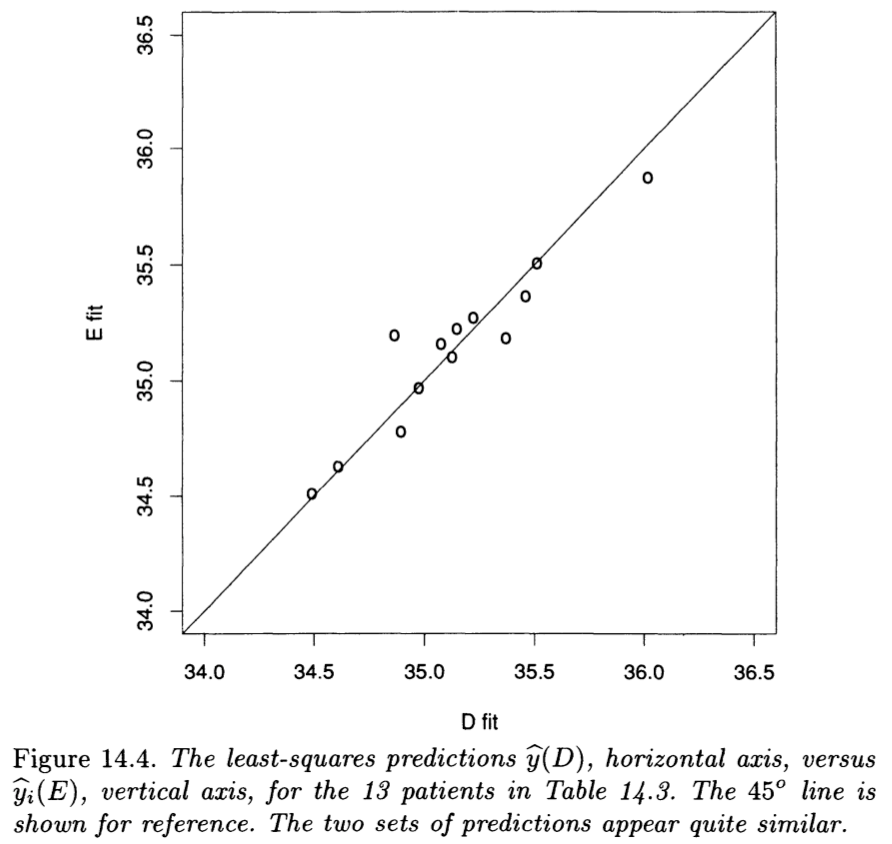
\includegraphics[width=0.85\linewidth]{14/f144.png}
\newline

В левой части рисунка 14.5 --- гистограмма 2000 репликаций непараметрического бутстрепа статистики RSE разности $\what \theta$, (14.31). Пусть $\mbf x = (\xes{13})$ представляет из себя матрицу данных из таблицы 14.3, где $x_i$ есть $i$-ый столбец матрицы, (14.25). Непараметрическая бутстреп выборка $\mbf x^* = (\xest{13})$ есть матрица, состоящая из строк, взятых с возвращением из совокупности $\{\xes{13}\}$. Это эквивалентно следующей записи:
\begin{equation}
  \what F \rightarrow\mbf x^* = (\xest{13}),
\end{equation}
где $\what F$ есть эмпирическая функция распределения, которая задает вероятность $1/13$ выбора каждой из строк $x_i$.

Следуя определениям из (14.25)--(14.30) бутстреп матрица $\mbf x^*$ приводит к $\mbf y^*$, $\mbf D^*$, $\what \beta(D)^*$, $\what y_i (D)^*$, а затем

\begin{equation}
  \rse(D)^* = \summ{i = 1}{13} (y_i^* - \what y_i(D)^*)^2,
\end{equation}
и аналогично $\rse(E)^* = \summ{i = 1}{13} (y_i^* - \what y_i(E)^*)^2$. Бутстреп репликация $\what \theta$ будет иметь вид
\begin{equation}
  \what \theta^* = \frac{1}{13}[\rse(E)^* - \rse(D)^*].
\end{equation}
Как и всегда, $\what \theta^*$ вычисляется с помощью того же алгоритма, что и исходная оценка $\what \theta$. Меняется лишь матрица данных $\mbf x$ на $\mbf x^*$ и вектор $\mbf y$ на $\mbf y^*$. 

Бутстреп гистограмма содержит информацию, которая нам необходима для ответа на вопросы  о значимости и важности $\what \theta$. Даже без построения доверительных интервалов можно получить некоторые ответы. Бутстреп оценка стандартной ошибки (6.6) равна
\begin{equation}
  \what{\tx{se}}_{2000} = 0.0311.
\end{equation}
Это означает, что $\what \theta = 0.0285$ менее чем на одну стандартную ошибку отстоит от нуля, откуда можно сделать вывод о том, что нам не следует ожидать серьезных оснований отвергнуть гипотезу о том, что истинное значение $\theta$ равно 0. С другой стороны, оценка смещена вниз ($62\%$ значений $\what \theta^*$ оказываются меньшими, чем $\what \theta^*$). Это указывает на то, что уровень значимости окажется больше $0.18 = 1 - \Phi(0.0285/0.0311)$, в условиях нормальной аппроксимации $\what \theta \sim N(\theta,0.0311^2)$.

Бутстреп гистограмма указывает на то, что $\theta$ оказывается не более $0.10$. Насколько существенна эта разница? Для этого нужно понять что именно измеряет параметр $\theta$.    Если $F$ есть истинное пятимерное распределение вектора $(d_1,d_2,e_1,e_2,y)$, то
\begin{align}
	\theta_D &= \min_{\beta_D} \tx{E}_F [y - (\beta_{D_0} + \beta_{D_1}d_1 + \beta_{D_0}d_2)]^2, \notag\\
	\theta_E &= \min_{\beta_E} \tx{E}_F [y - (\beta_{E_0} + \beta_{E_1}e_1 + \beta_{E_0}e_2)]^2
\end{align}
--- есть истинное значение ошибок предсказания при использовании переменных $D$ и $E$, соответственно. Параметр $\theta$, соответствующий $\what \theta$ есть
\begin{equation}
  \theta = \theta_E - \theta_D.
\end{equation}
Оценка $\theta_D$ по методу подстановки --- $\what \theta_D = \rse(D)/13 = 0.212$. Наша гипотеза о том, что $\theta \leqslant 0.10$ приводит к 
\begin{equation}
  \frac{\theta_E - \theta_D}{\theta_D} \dot = \frac{\theta_E - \theta_D}{\what \theta_D} < \frac{0.10}{0.212} = 0.47.
\end{equation}
Можно сделать вывод о том, что переменные E вероятно не лучше, чем переменные D для предсказания твердости, и вероятно не более чем на $50\%$ хуже.

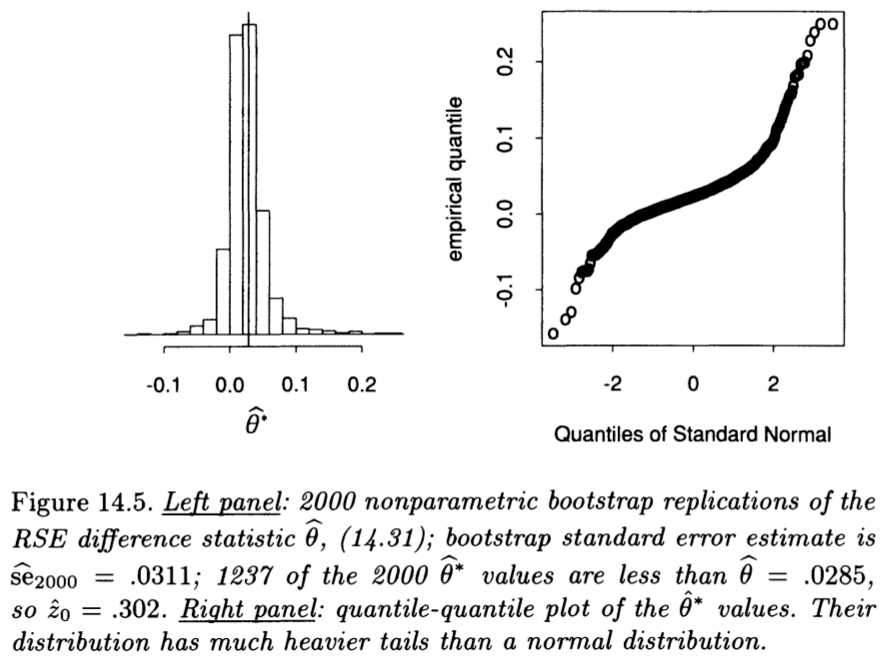
\includegraphics[width=0.85\linewidth]{14/f145.png}
\newline

В первом столбце таблицы 14.4 указаны доверительные интервалы для $\theta$ по методу $\bca$ на основе 2000 репликаций непараметрического бутстрепа.

Доверительные границы $\what \theta[\alpha]$ даны для восьми значений уровня значимости. Доверительные интервалы получаются взятием пар вида $(\what \theta[\alpha], \what \theta[1-\alpha])$ (например, $(\what \theta[0.05], \what \theta[0.95])$ --- $90\%$ интервал). Формулы (14.14) и (14.15) приводят к малому значению ускорения и большой поправке на смещение --- $\hat a = 0.040$ и $\hat z_0 = 0.47$.

Заметим, что непараметрическая граница для 0.05 положительна, $\what \theta[0.05] = 0.004$. Как говорилось ранее, это связано с большим значением поправки на смещение. Если бы $\bca$ метод был точным, мы могли бы утверждать, что нулевая гипотеза $\theta = 0$ отвергается при односторонеей критической области и уровне значимости $0.05$. Метод не точный, поэтому следует быть осторожнее с выводами. Непараметрические $\bca$ интервалы часто оказываются немного короткими, в особенности в случаях малой выборки (как в этом примере). Если бы проверка гипотезы имела критическое значение, то возможно добиться улучшения уровня значимости посредством калибровке, как в разделе 25.6.

\noindent
\begin{center}
\includegraphics[width=0.9\linewidth]{14/t144.png}
\end{center}
\setcounter{table}{3}

Для проверки непараметрических интервалов было построено еще 2000 бутстреп выборок, в данном случае основанных на нормальной модели; предполагается, что строки $x_i$ матрицы данных были получены моделированием из пятимерного нормального распределения $F_\tx{norm}$. Далее было найдено наилучшее аппроксимирующее данные распределение $\what F_\tx{norm}$, а затем сгенерированы выборки $\mbf x^*$ из $\what F_\tx{norm}$ как в (14.7). Гистограмма на основе 2000 бутстреп репликаций параметрического бутстрепа показана на левой стороне рисунка 14.6; она похожа на гистограмму из рисунка 14.5 (за исключением того, что в данном случае хвосты менее тяжелые).

$\bca$ интервалы вычислены так же, как и ранее, используя формулы (14.9) и (14.10). Формула поправки на смещение (14.14) также не изменилась. Параметр ускорения $\hat a$ вычислен с помощью параметрической версии формулы (14.15), взятой из алгоритма \texttt{abcpar} построения параметрических $\abc$ интервалов. В данном случае параметрические $\bca$ границы, указанные в центральной части таблицы 14.4, не сильно отличаются от своего непараметрического аналога. В то же время разница оказывается достаточно большой, такой, что гипотеза $\theta = 0$ уже не отвергается на уровне $0.05$ (при выборе одностороннего доверительного интервала).

\includegraphics[width=0.85\linewidth]{14/f146.png}
\newline

Непохоже, что исходные данные распределены нормально. Однако причиной использования бутстрепа с предположением нормальности заключается в малой размерности данных, $n=13$. Для слишком малых выборок бутстреп даже с неподходящей параметрической моделью может оказаться более успешным, уменьшив дисперсию результатов в ущерб допустимого смещения. В данном же примере результаты по двум методам весьма похожи.

В главе 9 рассматриваются модели линейной регрессии. Можем использовать модель линейной регрессии для того, чтобы предложить другой вариант бутстреп анализа разностной статистики $\hat \theta$. Используя обозначения из (14.25), пусть $c_i$ представляет из себя вектор
\begin{equation}
 \mbf c_i = (1,d_{1i},d_{2i}, e_{1i}, e_{2i});
\end{equation}
рассмотрим линейную модель (9.4), (9.5)
\begin{equation}
  y_i = \mbf c_i\mbf \beta + \varepsilon_i \qquad (\ies{13}).
\end{equation}
Бутстреп выборки $\mbf y^* = (y_1^*,y_2^*,\ldots,y_{13}^*)$ получены из остатков повторных выборок (как в (9.25) и (9.26)). Бутстреп репликации $\what \theta^*$ остаются такими же, как в (14.35). Следует заметить, что вычисление $\what y_i(D)^*$ и $\what y_i(E)^*$ несколько отличается.

На правой стороне рисунка 14.6 показано бутстреп распределение на основе 2000 репликаций $\what \theta^*$. Хвосты  у этой гистограммы легче, чем хвосты на рисунке 14.5. Это отражено и в таблице 14.4 --- соответствующие интервалы стали более узкими. Несмотря на это, гипотеза $\theta = 0$ 	отвергается реже, чем раньше: при уровне $\alpha = 0.16$. Это происходит из-за того, что $\what \theta$ уже не выглядит смещенной вниз, $\what z_0$ равен $0.059$, а не $0.302$, как в непараметрическом случае.

Доверительные интервалы и проверка гипотез являются <<деликатными>> инструментами статистической теории выводов. В этой связи они сильнее зависят от выбора модели, чем обычные стандартные ошибки. В особенности эти соображения верны для случаев, когда размер выборки мал. Исследование зависимостей между пятью переменными на основе 13 наблюдений очевидно является задачей с малым размером выборки. Даже если бы $\bca$ интервалы были точными (а это не так), то изменение модели приводило бы к другим доверительным интервалам, что видно из таблицы 14.4.

В таблице 14.4 показаны $\abc$ интервалы для трёх различных вариантов выбора модели. Результаты были получены с использованием реализаций программ \texttt{abcnon} и \texttt{abcpar} из приложения. Непараметрические $\abc$ интервалы оказываются слишком короткими в данном случае. Это происходит из-за необычно тяжелых хвостов у распределения непараметрического бустстрепа. Если говорить на языке статистики, то метод $\abc$ может исправить асимметрию распределения, но не его эксцесс (это все, что требуется для достижения точности второго порядка). Асимптиотическая точность метода $\abc$ не гарантирует его успешность на малых выборках.

Стандартные ошибки $\what \theta$ даны для каждого из шести столбцов в таблице 14.4. Приведенные для $\bca$ --- это классические бутстреп стандартные ошибки. Стандартные ошибки для $\abc$ получены с помощью дельта метода из главы 21 (похожего на метод вычисления стандартной ошибки по методу складного ножа, (11.5)). Стандартная ошибка $\bca$ более чем в два раза превышает ошибку по методу $\abc$ в непараметрическом случае, что свидетельствует о том, что интервалы $\abc$ будут слишком короткими. (Большая $\bca$ стандартная ошибка стала заметна уже после первых 100 бутстреп репликаций.) Обычно аппроксимация по методу $\abc$ работает удовлетворительно как в таблице 14.2. Однако в любом случае может оказаться полезной проверка стандартных ошибок используя небольшое число бутстреп репликаций (например, 100).

 






\end{document}
